
%Futuring Study material template- This template is designed for the soft copy
%This template is for the subject PHYSICS ONLY
%----------------------------------------------------------------------------------------
%	PACKAGES AND OTHER DOCUMENT CONFIGURATIONS
%----------------------------------------------------------------------------------------

\documentclass[11pt,twoside]{book} % Default font size and left-justified equations

%%%
%----------------------------------------------------------------------------------------
%	VARIOUS REQUIRED PACKAGES AND CONFIGURATIONS
%----------------------------------------------------------------------------------------
\usepackage{eucal}
\usepackage{setspace}
\usepackage{bigints}
\usepackage{etoolbox}
\usepackage{dirtytalk}
\usepackage{epigraph}
\usepackage{physics}
\usepackage{amssymb}
\usepackage{chemfig}
\usepackage{stackrel}
\usepackage{scalerel}
\usepackage{longtable}
\usepackage{tabularx}
\usepackage{caption}
\usepackage{multirow}
\usepackage{environ}
\usepackage{subfigure}
\usepackage{graphicx} % Required for including pictures
\graphicspath{{Pictures/}{Pictures/sketching/}{Pictures/single and complex/}{Pictures/Coordinate system/}{Pictures/vector/}{Pictures/jamfigure/}{Pictures/conicsection/}{Pictures/conicsection/}{Pictures/electrostatics/}{Pictures/LCR/} {Pictures/BHU/}{Pictures/HCU/}{Pictures/Jest/}{Pictures/magnetostatics/}{Pictures/p-coulombs law/}{Pictures/p-vector/}{Pictures/quantum/}{Pictures/}{Pictures/BHU/}{Pictures/HCU/}{Pictures/JEST/} {Pictures/STR/}{Pictures/nuclear/} {Pictures/quantum/} {Pictures/Particle/} {Pictures/Newtons law/} {Pictures/work and energy/} {Pictures/Kinematics/}{Pictures/math prelim/} {Pictures/semiconductors/}{Pictures/Fluid mechanics/}{Pictures/Bipolar junction transistor/}{Pictures/Solid state/}{Pictures/digital/}{Pictures/Waves/}{Pictures/OPAMP/}{Pictures/Optics/}{Pictures/Wave Optics/}{Pictures/Net/}{Pictures/NET/}{Pictures/Gate/}{pictures/Newtons law/}{pictures/Kinematics/}{pictures/work and energy/}{pictures/jamfigure/}{Pictures/Problems/} {Pictures/Dirac delta function/}{Pictures/Differential equations/}{Pictures/Assignment/}{Pictures/Assignments/}
{Pictures/Electronics-CSIR/} {Pictures/CM/} {Pictures/Statistical Physics/}{Pictures/Digital Electronics/}{Pictures/Relativity and Electromagnetism/}{Pictures/Net 2019/}}
 % Specifies the directory where pictures are stored
\usepackage{float}
\usepackage{lipsum} % Inserts dummy text
\usepackage{wrapfig}
\usepackage{tikz} % Required for drawing custom shapes
\usepackage{amsmath}
 % English language/hyphenation

\usepackage{enumitem}
\newlist{questions}{enumerate}{3}
\setlist[questions]{wide=0pt, leftmargin=15pt, labelwidth=15pt, labelsep=0pt, align=left,label=\color{futuringtheme}\bfseries\large\arabic*.}
\newcommand{\question}{\item}


%\AtBeginEnvironment{enumerate}{\linespread{6.84}\selectfont}

 
 
\NewEnviron{abox}{%
	\begin{center}
\begin{tikzpicture}
\node[align=center,anchor=base,draw,rectangle,text width=\textwidth,line width=2pt,rounded corners=15pt,draw=ocre,fill=white,fill opacity=0.9,inner sep=10pt] 
{\centering \textbf{ \huge \color{futuringtheme}\BODY}};
\end{tikzpicture}

	\end{center}
	
	
}
\newcommand{\exyear}[1]{\newline \llap{}\hfill \color{futuringtheme}{\textbf{[#1]}}}
\usepackage{booktabs} % Required for nicer horizontal rules in tables
\usepackage{tasks}
\usepackage{xcolor} % Required for specifying colors by name
\definecolor{ocre}{RGB}{243,102,25} % Define the orange color used for highlighting throughout the book
\definecolor{futuringtheme}{RGB}{0,142,212}
%----------------------------------------------------------------------------------------
%..............................Added packages
\usepackage{import}
\usepackage{array}
\usepackage{colortbl}
\usepackage{cutwin}

\usepackage[printwatermark]{xwatermark}

\newsavebox\mylogobox
\savebox\mylogobox{\tikz[opacity=0.2]\node[inner sep=0pt] (russell) at (0,0)
	{
\includegraphics[width=3cm]{../Config/Pictures/logotra2.png}};}
\newwatermark*[
allpages,
angle=0,
scale=5,
xpos=0,
ypos=0
]{\usebox\mylogobox}



%.........................
%	MARGINS
%----------------------------------------------------------------------------------------
\usepackage{tasks}
\usepackage{geometry} % ccbyRequired for adjusting page dimensions and margins

\geometry{
	paper=a4paper, % Paper size, change to letterpaper for US letter size
	top=2cm, % Top margin
	bottom=2cm, % Bottom margin
	left=2cm, % Left margin
	right=2cm, % Right margin
	headheight=14pt, % Header height
	footskip=1.4cm, % Space from the bottom margin to the baseline of the footer
	headsep=10pt, % Space from the top margin to the baseline of the header
	%showframe, % Uncomment to show how the type block is set on the page
}

\allowdisplaybreaks
\makeatletter
\def\SetTotalwidth{\advance\linewidth by \@totalleftmargin
	\@totalleftmargin=0pt}
\makeatother

%----------------------------------------------------------------------------------------
%y

\usepackage{avant} % Use the Avantgarde font for headings
%\usepackage{times} % Use the Times font for headings
\usepackage{mathptmx} % Use the Adobe Times Roman as the default text font together with math symbols from the Sym­bol, Chancery and Com­puter Modern fonts

\usepackage{microtype} % Slightly tweak font spacing for aesthetics
\usepackage[utf8]{inputenc} % Required for including letters with accents
\usepackage[T1]{fontenc} % Use 8-bit encoding that has 256 glyphs

%----------------------------------------------------------------------------------------
%	BIBLIOGRAPHY AND INDEX
%----------------------------------------------------------------------------------------


%----------------------------------------------------------------------------------------
%	MAIN TABLE OF CONTENTS
%----------------------------------------------------------------------------------------

\usepackage{titletoc} % Required for manipulating the table of contents

\contentsmargin{0cm} % Removes the default margin

% Part text styling (this is mostly taken care of in the PART HEADINGS section of this file)
\titlecontents{part}
	[0cm] % Left indentation
	{\addvspace{20pt}\bfseries} % Spacing and font options for parts
	{}
	{}
	{}

% Chapter text styling
\titlecontents{chapter}
	[1.25cm] % Left indentation
	{\addvspace{12pt}\large\sffamily\bfseries} % Spacing and font options for chapters
	{\color{ocre!60}\contentslabel[\Large\thecontentslabel]{1.25cm}\color{ocre}} % Formatting of numbered sections of this type
	{\color{ocre}} % Formatting of numberless sections of this type
	{\color{ocre!60}\normalsize\;\titlerule*[.5pc]{.}\;\thecontentspage} % Formatting of the filler to the right of the heading and the page number

% Section text styling
\titlecontents{section}
	[1.25cm] % Left indentation
	{\addvspace{3pt}\sffamily\bfseries} % Spacing and font options for sections
	{\contentslabel[\thecontentslabel]{1.25cm}} % Formatting of numbered sections of this type
	{} % Formatting of numberless sections of this type
	{\hfill\color{black}\thecontentspage} % Formatting of the filler to the right of the heading and the page number

% Subsection text styling
\titlecontents{subsection}
	[1.25cm] % Left indentation
	{\addvspace{1pt}\sffamily\small} % Spacing and font options for subsections
	{\contentslabel[\thecontentslabel]{1.25cm}} % Formatting of numbered sections of this type
	{} % Formatting of numberless sections of this type
	{\ \titlerule*[.5pc]{.}\;\thecontentspage} % Formatting of the filler to the right of the heading and the page number

% Figure text styling
\titlecontents{figure}
	[1.25cm] % Left indentation
	{\addvspace{1pt}\sffamily\small} % Spacing and font options for figures
	{\thecontentslabel\hspace*{1em}} % Formatting of numbered sections of this type
	{} % Formatting of numberless sections of this type
	{\ \titlerule*[.5pc]{.}\;\thecontentspage} % Formatting of the filler to the right of the heading and the page number

% Table text styling
\titlecontents{table}
	[1.25cm] % Left indentation
	{\addvspace{1pt}\sffamily\small} % Spacing and font options for tables
	{\thecontentslabel\hspace*{1em}} % Formatting of numbered sections of this type
	{} % Formatting of numberless sections of this type
	{\ \titlerule*[.5pc]{.}\;\thecontentspage} % Formatting of the filler to the right of the heading and the page number

%----------------------------------------------------------------------------------------
%	MINI TABLE OF CONTENTS IN PART HEADS
%----------------------------------------------------------------------------------------

% Chapter text styling
\titlecontents{lchapter}
	[0em] % Left indentation
	{\addvspace{15pt}\large\sffamily\bfseries} % Spacing and font options for chapters
	{\color{ocre}\contentslabel[\Large\thecontentslabel]{1.25cm}\color{ocre}} % Chapter number
	{}  
	{\color{ocre}\normalsize\sffamily\bfseries\;\titlerule*[.5pc]{.}\;\thecontentspage} % Page number

% Section text styling
\titlecontents{lsection}
	[0em] % Left indentation
	{\sffamily\small} % Spacing and font options for sections
	{\contentslabel[\thecontentslabel]{1.25cm}} % Section number
	{}
	{}

% Subsection text styling (note these aren't shown by default, display them by searchings this file for tocdepth and reading the commented text)
\titlecontents{lsubsection}
	[.5em] % Left indentation
	{\sffamily\footnotesize} % Spacing and font options for subsections
	{\contentslabel[\thecontentslabel]{1.25cm}}
	{}
	{}

%----------------------------------------------------------------------------------------
%	HEADERS AND FOOTERS
%----------------------------------------------------------------------------------------

\usepackage{fancyhdr} % Required for header and footer configuration

\pagestyle{fancy} % Enable the custom headers and footers

\renewcommand{\chaptermark}[1]{\markboth{\sffamily\normalsize\bfseries\chaptername\ \thechapter.\ #1}{}} % Styling for the current chapter in the header
\renewcommand{\sectionmark}[1]{\markright{\sffamily\normalsize\thesection\hspace{5pt}#1}{}} % Styling for the current section in the header

\fancyhf{} % Clear default headers and footers
\fancyhead[LE,RO]{\sffamily\normalsize\thepage} % Styling for the page number in the header
\fancyhead[LO]{\rightmark} % Print the nearest section name on the left side of odd pages
\fancyhead[RE]{\leftmark} % Print the current chapter name on the right side of even pages
\renewcommand{\headrulewidth}{0.5pt} % Thickness of the rule under the header


% Removes the header from odd empty pages at the end of chapters
\makeatletter
\renewcommand{\cleardoublepage}{
\clearpage\ifodd\c@page\else
\hbox{}
\vspace*{\fill}
\thispagestyle{empty}
\newpage
\fi}


\fancypagestyle{plain}{% Redefine plain pages tyle
	\fancyhf{}% Clear header/footer
	
	\fancyhead[LE,RO]{\sffamily\normalsize\thepage}
	 % Print the nearest section name on the left side of odd pages
	\fancyhead[RE]{\leftmark}
}

%----------------------------------------------------------------------------------------

%Box Styles
\usepackage{tcolorbox}
\newtcolorbox{myboxthree}{colback=futuringtheme!5!white,colframe=ocre!75}






















%	THEOREM STYLES
%----------------------------------------------------------------------------------------

\usepackage{amsmath,amsfonts,amssymb,amsthm} % For math equations, theorems, symbols, etc

\newcommand{\intoo}[2]{\mathopen{]}#1\,;#2\mathclose{[}}
\newcommand{\ud}{\mathop{\mathrm{{}d}}\mathopen{}}
\newcommand{\intff}[2]{\mathopen{[}#1\,;#2\mathclose{]}}
\renewcommand{\qedsymbol}{$\blacksquare$}
\newtheorem{notation}{Notation}[chapter]

% Boxed/framed environments
\newtheoremstyle{ocrenumbox}% Theorem style name
{0pt}% Space above
{0pt}% Space below
{\normalfont}% Body font
{}% Indent amount
{\small\bf\sffamily\color{ocre}}% Theorem head font
{\;}% Punctuation after theorem head
{0.25em}% Space after theorem head
{\small\sffamily\color{ocre}\thmname{#1}\nobreakspace\thmnumber{\@ifnotempty{#1}{}\@upn{#2}}% Theorem text (e.g. Theorem 2.1)
\thmnote{\nobreakspace\the\thm@notefont\sffamily\bfseries\color{black}---\nobreakspace#3.}} % Optional theorem note

\newtheoremstyle{blacknumex}% Theorem style name
{5pt}% Space above
{5pt}% Space below
{\normalfont}% Body font
{} % Indent amount
{\small\bf\sffamily}% Theorem head font
{\;}% Punctuation after theorem head
{0.25em}% Space after theorem head
{\small\sffamily{\tiny\ensuremath{\blacksquare}}\nobreakspace\thmname{#1}\nobreakspace\thmnumber{\@ifnotempty{#1}{}\@upn{#2}}% Theorem text (e.g. Theorem 2.1)
\thmnote{\nobreakspace\the\thm@notefont\sffamily\bfseries---\nobreakspace#3.}}% Optional theorem note

\newtheoremstyle{blacknumbox} % Theorem style name
{0pt}% Space above
{0pt}% Space below
{\normalfont}% Body font
{}% Indent amount
{\small\bf\sffamily}% Theorem head font
{\;}% Punctuation after theorem head
{0.25em}% Space after theorem head
{\small\sffamily\thmname{#1}\nobreakspace\thmnumber{\@ifnotempty{#1}{}\@upn{#2}}% Theorem text (e.g. Theorem 2.1)
\thmnote{\nobreakspace\the\thm@notefont\sffamily\bfseries---\nobreakspace#3.}}% Optional theorem note

% Non-boxed/non-framed environments
\newtheoremstyle{ocrenum}% Theorem style name
{5pt}% Space above
{5pt}% Space below
{\normalfont}% Body font
{}% Indent amount
{\small\bf\sffamily\color{ocre}}% Theorem head font
{\;}% Punctuation after theorem head
{0.25em}% Space after theorem head
{\small\sffamily\color{ocre}\thmname{#1}\nobreakspace\thmnumber{\@ifnotempty{#1}{}\@upn{#2}}% Theorem text (e.g. Theorem 2.1)
\thmnote{\nobreakspace\the\thm@notefont\sffamily\bfseries\color{black}---\nobreakspace#3.}} % Optional theorem note
\makeatother

%Box style for Solution environment
\newtheoremstyle{solbox}% Theorem style name
{0pt}% Space above
{0pt}% Space below
{\normalfont}% Body font
{}% Indent amount
{\small\bf\sffamily\color{ocre}}% Theorem head font
{\;}% Punctuation after theorem head
{0.25em}% Space after theorem head
{\small\sffamily\color{ocre}Solution:}


% Defines the theorem text style for each type of theorem to one of the three styles above
\newcounter{dummy} 
\numberwithin{dummy}{section}
\theoremstyle{ocrenumbox}
\newtheorem{theoremeT}[dummy]{Theorem}
\newtheorem{problem}{Problem}[chapter]
\newtheorem{exerciseT}{Exercise}[chapter]
\theoremstyle{blacknumex}
\newtheorem{exampleT}{Example}[chapter]
\theoremstyle{blacknumbox}
\newtheorem{vocabulary}{Vocabulary}[chapter]
\newtheorem{definitionT}{Definition}[section]
\newtheorem{corollaryT}[dummy]{Corollary}
\theoremstyle{ocrenum}
\newtheorem{proposition}[dummy]{Proposition}
\theoremstyle{solbox}
\newtheorem{answerT}[dummy]{Solution}

%----------------------------------------------------------------------------------------
%	DEFINITION OF COLORED BOXES
%----------------------------------------------------------------------------------------

\RequirePackage[framemethod=default]{mdframed} % Required for creating the theorem, definition, exercise and corollary boxes

% Theorem box
\newmdenv[skipabove=7pt,
skipbelow=7pt,
backgroundcolor=white,
linecolor=ocre,
innerleftmargin=5pt,
innerrightmargin=5pt,
innertopmargin=10pt,
leftmargin=0cm,
rightmargin=0cm,
innerbottommargin=5pt]{tBox}

% Exercise box	  
\newmdenv[skipabove=7pt,
skipbelow=7pt,
rightline=false,
leftline=true,
topline=false,
bottomline=false,
backgroundcolor=ocre!10,
linecolor=ocre,
innerleftmargin=5pt,
innerrightmargin=5pt,
innertopmargin=5pt,
innerbottommargin=5pt,
leftmargin=0cm,
rightmargin=0cm,
linewidth=4pt]{eBox}	

% Definition box
\newmdenv[skipabove=7pt,
skipbelow=7pt,
rightline=false,
leftline=true,
topline=false,
bottomline=false,
linecolor=ocre,
innerleftmargin=5pt,
innerrightmargin=5pt,
innertopmargin=0pt,
leftmargin=0cm,
rightmargin=0cm,
linewidth=4pt,
innerbottommargin=0pt]{dBox}	

% Corollary box
\newmdenv[skipabove=7pt,
skipbelow=7pt,
rightline=false,
leftline=true,
topline=false,
bottomline=false,
linecolor=gray,
backgroundcolor=black!5,
innerleftmargin=5pt,
innerrightmargin=5pt,
innertopmargin=5pt,
leftmargin=0cm,
rightmargin=0cm,
linewidth=4pt,
innerbottommargin=5pt]{cBox}

% Creates an environment for each type of theorem and assigns it a theorem text style from the "Theorem Styles" section above and a colored box from above
\newenvironment{theorem}{\begin{tBox}\begin{theoremeT}}{\end{theoremeT}\end{tBox}}
\newenvironment{exercise}{\begin{eBox}\begin{exerciseT}}{\hfill{\color{ocre}\tiny\ensuremath{\blacksquare}}\end{exerciseT}\end{eBox}}				  
\newenvironment{definition}{\begin{dBox}\begin{definitionT}}{\end{definitionT}\end{dBox}}	
\newenvironment{example}{\begin{exampleT}}{\hfill{\tiny\ensuremath{\blacksquare}}\end{exampleT}}		
\newenvironment{corollary}{\begin{cBox}\begin{corollaryT}}{\end{corollaryT}\end{cBox}}	
\newenvironment{answer}{\begin{tBox}\begin{answerT}}{\end{answerT}\end{tBox}}	

%----------------------------------------------------------------------------------------
%	REMARK ENVIRONMENT
%----------------------------------------------------------------------------------------

\newenvironment{remark}{\par\vspace{10pt}\normlasize % Vertical white space above the remark and smaller font size
\begin{list}{}{
\leftmargin=35pt % Indentation on the left
\rightmargin=25pt}\item\ignorespaces % Indentation on the right
\makebox[-2.5pt]{\begin{tikzpicture}[overlay]
\node[draw=ocre!60,line width=1pt,circle,fill=ocre!25,font=\sffamily\bfseries,inner sep=2pt,outer sep=0pt] at (-15pt,0pt){\textcolor{ocre}{R}};\end{tikzpicture}} % Orange R in a circle
\advance\baselineskip -1pt}{\end{list}\vskip5pt} % Tighter line spacing and white space after remark

\newenvironment{note}{\par\vspace{10pt}\normalsize % Vertical white space above the remark and smaller font size
	\begin{list}{}{
			\leftmargin=35pt % Indentation on the left
			\rightmargin=25pt}\item\ignorespaces % Indentation on the right
		\makebox[-2.5pt]{\begin{tikzpicture}[overlay]
			\node[draw=ocre!60,line width=1pt,rectangle,fill=ocre!25,font=\sffamily\bfseries,inner sep=2pt,outer sep=0pt] at (-15pt,0pt){\textcolor{ocre}{Note}};\end{tikzpicture}} % Orange R in a circle
		\advance\baselineskip -5pt}{\end{list}\vskip5pt} % Tighter line spacing and white space after remark

%----------------------------------------------------------------------------------------
%	SECTION NUMBERING IN THE MARGIN
%----------------------------------------------------------------------------------------

\makeatletter
\renewcommand{\@seccntformat}[1]{\llap{\textcolor{ocre}{\csname the#1\endcsname}\hspace{1em}}}                    
\renewcommand{\section}{\@startsection{section}{1}{\z@}
{-4ex \@plus -1ex \@minus -.4ex}
{1ex \@plus.2ex }
{\normalfont\large\sffamily\bfseries}}
\renewcommand{\subsection}{\@startsection {subsection}{2}{\z@}
{-3ex \@plus -0.1ex \@minus -.4ex}
{0.5ex \@plus.2ex }
{\normalfont\sffamily\bfseries}}
\renewcommand{\subsubsection}{\@startsection {subsubsection}{3}{\z@}
{-2ex \@plus -0.1ex \@minus -.2ex}
{.2ex \@plus.2ex }
{\normalfont\small\sffamily\bfseries}}                        
\renewcommand\paragraph{\@startsection{paragraph}{4}{\z@}
{-2ex \@plus-.2ex \@minus .2ex}
{.1ex}
{\normalfont\small\sffamily\bfseries}}

%----------------------------------------------------------------------------------------
%	PART HEADINGS
%----------------------------------------------------------------------------------------

% Numbered part in the table of contents
\newcommand{\@mypartnumtocformat}[2]{%
	\setlength\fboxsep{0pt}%
	\noindent\colorbox{ocre!20}{\strut\parbox[c][.7cm]{\ecart}{\color{ocre!70}\Large\sffamily\bfseries\centering#1}}\hskip\esp\colorbox{ocre!40}{\strut\parbox[c][.7cm]{\linewidth-\ecart-\esp}{\Large\sffamily\centering#2}}%
}

% Unnumbered part in the table of contents
\newcommand{\@myparttocformat}[1]{%
	\setlength\fboxsep{0pt}%
	\noindent\colorbox{ocre!40}{\strut\parbox[c][.7cm]{\linewidth}{\Large\sffamily\centering#1}}%
}

\newlength\esp
\setlength\esp{4pt}
\newlength\ecart
\setlength\ecart{1.2cm-\esp}
\newcommand{\thepartimage}{}%
\newcommand{\partimage}[1]{\renewcommand{\thepartimage}{#1}}%
\def\@part[#1]#2{%
\ifnum \c@secnumdepth >-2\relax%
\refstepcounter{part}%
\addcontentsline{toc}{part}{\texorpdfstring{\protect\@mypartnumtocformat{\thepart}{#1}}{\partname~\thepart\ ---\ #1}}
\else%
\addcontentsline{toc}{part}{\texorpdfstring{\protect\@myparttocformat{#1}}{#1}}%
\fi%
\startcontents%
\markboth{}{}%
{\thispagestyle{empty}%
\begin{tikzpicture}[remember picture,overlay]%
\node at (current page.north west){\begin{tikzpicture}[remember picture,overlay]%	
\fill[ocre!20](0cm,0cm) rectangle (\paperwidth,-\paperheight);
\node[anchor=north] at (4cm,-3.25cm){\color{ocre!40}\fontsize{220}{100}\sffamily\bfseries\thepart}; 
\node[anchor=south east] at (\paperwidth-1cm,-\paperheight+1cm){\parbox[t][][t]{8.5cm}{
\printcontents{l}{0}{\setcounter{tocdepth}{1}}% The depth to which the Part mini table of contents displays headings; 0 for chapters only, 1 for chapters and sections and 2 for chapters, sections and subsections
}};
\node[anchor=north east] at (\paperwidth-1.5cm,-3.25cm){\parbox[t][][t]{15cm}{\strut\raggedleft\color{white}\fontsize{30}{30}\sffamily\bfseries#2}};
\end{tikzpicture}};
\end{tikzpicture}}%
\@endpart}
\def\@spart#1{%
\startcontents%
\phantomsection
{\thispagestyle{empty}%
\begin{tikzpicture}[remember picture,overlay]%
\node at (current page.north west){\begin{tikzpicture}[remember picture,overlay]%	
\fill[ocre!20](0cm,0cm) rectangle (\paperwidth,-\paperheight);
\node[anchor=north east] at (\paperwidth-1.5cm,-3.25cm){\parbox[t][][t]{15cm}{\strut\raggedleft\color{white}\fontsize{30}{30}\sffamily\bfseries#1}};
\end{tikzpicture}};
\end{tikzpicture}}
\addcontentsline{toc}{part}{\texorpdfstring{%
\setlength\fboxsep{0pt}%
\noindent\protect\colorbox{ocre!40}{\strut\protect\parbox[c][.7cm]{\linewidth}{\Large\sffamily\protect\centering #1\quad\mbox{}}}}{#1}}%
\@endpart}
\def\@endpart{\vfil\newpage
\if@twoside
\if@openright
\null
\thispagestyle{empty}%
\newpage
\fi
\fi
\if@tempswa
\twocolumn
\fi}

%----------------------------------------------------------------------------------------
%	CHAPTER HEADINGS
%----------------------------------------------------------------------------------------

% A switch to conditionally include a picture, implemented by Christian Hupfer
\newif\ifusechapterimage
\usechapterimagetrue
\newcommand{\thechapterimage}{}%
\newcommand{\chapterimage}[1]{\ifusechapterimage\renewcommand{\thechapterimage}{#1}\fi}%
\newcommand{\autodot}{.}
\def\@makechapterhead#1{%
{\parindent \z@ \raggedright \normalfont
\ifnum \c@secnumdepth >\m@ne
\if@mainmatter
\begin{tikzpicture}[remember picture,overlay]
\node at (current page.north west)
{\begin{tikzpicture}[remember picture,overlay]
\node[anchor=north west,inner sep=0pt] at (0,0) {\ifusechapterimage\includegraphics[width=\paperwidth]{\thechapterimage}\fi};
\draw[anchor=west] (\Gm@lmargin,-9cm) node [line width=2pt,rounded corners=15pt,draw=ocre,fill=white,fill opacity=0.5,inner sep=15pt]{\strut\makebox[22cm]{}};
\draw[anchor=west] (\Gm@lmargin+.3cm,-9cm) node {\huge\sffamily\bfseries\color{black}\thechapter\autodot~#1\strut};
\end{tikzpicture}};
\end{tikzpicture}
\else
\begin{tikzpicture}[remember picture,overlay]
\node at (current page.north west)
{\begin{tikzpicture}[remember picture,overlay]
\node[anchor=north west,inner sep=0pt] at (0,0) {\ifusechapterimage\includegraphics[width=\paperwidth]{\thechapterimage}\fi};
\draw[anchor=west] (\Gm@lmargin,-9cm) node [line width=2pt,rounded corners=15pt,draw=ocre,fill=white,fill opacity=0.5,inner sep=15pt]{\strut\makebox[22cm]{}};
\draw[anchor=west] (\Gm@lmargin+.3cm,-9cm) node {\huge\sffamily\bfseries\color{black}#1\strut};
\end{tikzpicture}};
\end{tikzpicture}
\fi\fi\par\vspace*{270\p@}}}

%-------------------------------------------

\def\@makeschapterhead#1{%
\begin{tikzpicture}[remember picture,overlay]
\node at (current page.north west)
{\begin{tikzpicture}[remember picture,overlay]
\node[anchor=north west,inner sep=0pt] at (0,0) {\ifusechapterimage\includegraphics[width=\paperwidth]{\thechapterimage}\fi};
\draw[anchor=west] (\Gm@lmargin,-9cm) node [line width=2pt,rounded corners=15pt,draw=ocre,fill=white,fill opacity=0.5,inner sep=15pt]{\strut\makebox[22cm]{}};
\draw[anchor=west] (\Gm@lmargin+.3cm,-9cm) node {\huge\sffamily\bfseries\color{black}#1\strut};
\end{tikzpicture}};
\end{tikzpicture}
\par\vspace*{270\p@}}
\makeatother

%----------------------------------------------------------------------------------------
%	LINKS
%----------------------------------------------------------------------------------------

\usepackage{hyperref}
\hypersetup{hidelinks,backref=true,pagebackref=true,hyperindex=true,colorlinks=false,breaklinks=true,urlcolor=ocre,bookmarks=true,bookmarksopen=false}

\usepackage{bookmark}
\bookmarksetup{
open,
numbered,
addtohook={%
\ifnum\bookmarkget{level}=0 % chapter
\bookmarksetup{bold}%
\fi
\ifnum\bookmarkget{level}=-1 % part
\bookmarksetup{color=ocre,bold}%
\fi
}
}
 % Insert the commands.tex file which contains the majority of the structure behind the template

\hypersetup{pdftitle={Title},pdfauthor={Futuring}} % Uncomment and fill out to include PDF metadata for the author and title of the book

%----------------------------------------------------------------------------------------

\begin{document}
\chapterimage{../../Config/Pictures/one.jpg}
%----------------------------------------------------------------------------------------
%	TITLE PAGE
%----------------------------------------------------------------------------------------

%Place the content from the snippet file titlepage and fill out the details -- Titlepage details
%----------------------------------------------------------------------------------------
%	COPYRIGHT PAGE
%----------------------------------------------------------------------------------------

%Place the content from the snippet file copyrightpage and fill out the details -- copyright details

%----------------------------------------------------------------------------------------
%	TABLE OF CONTENTS
%----------------------------------------------------------------------------------------



%----------------------------------------------------------------------------------------
%	CHAPTER 1
%----------------------------------------------------------------------------------------



\chapter{Differential Equations}
In physics we encounter differential equations all the time. In fact the whole programme of classical mechanics is to develop a second order differential equation using Newton's laws of motion and then solving it.\\Sometimes these are ordinary
differential equations in one variable (abbreviated ODEs). More often the equations are
partial differential equations (PDEs) in two or more variables. Simply we can say , differential equations is a relation between a function and its derivatives.
\begin{definition}
	A differential equation is an equation which involves independent and dependent variables and their derivatives or differentials.
\end{definition}
\begin{example}
	\hspace{1cm}
\begin{itemize}
		\item $\frac{dy}{dx}={4x-2}$
		\item $\frac{d^{2}y}{dx^{2}}=5\frac{dy}{dx}+10$
		\item $(1+\frac{dy}{dx})^{3}=k\frac{dy}{dx}$
		\item $\frac{dy}{dx}+xy=x^{3}y^{3}$
		\item $\frac{\partial^{2}y}{\partial^{2} x}=\frac{1}{c^{2}} \frac{\partial^{2}y}{\partial^{2} x} $
		\item $\frac{\partial u}{\partial t}=\frac{\partial u}{\partial x}+\frac{\partial u}{\partial y}$
	\end{itemize}
\end{example}
\section{{Types of differential equation}}
There are mainly two types of differential equations,
	\begin{itemize}
	\item \textbf{Ordinary differential equations.}\par A differentnial equation involving derivatives with respect to a single variable is called an ordinary differential equation. 
	\\\\
	\textbf{General form:} $\frac{d y}{d x}=f(x, y)=-\frac{P(x, y)}{Q(x, y)}$
	\begin{example}
		\begin{align*}
		F&=m\frac{d v}{dt}\\
		\frac{dy}{dx}+x&= 1
		\end{align*}
	\end{example}
	\item \textbf{Partial differential equations.}\par A differential equation involving partial derivatives with respect to more than one independent variable is called a partial differential equation.
	\begin{example}
		\begin{align*}
		\intertext{\textbf{Poisson's equation:}}
		\nabla^{2}\psi&= \frac{\rho}{\epsilon_{0}}\\
		\left( \frac{\partial ^{2}}{\partial x^{2}}+\frac{\partial ^{2}}{\partial y^{2}}+\frac{\partial ^{2}}{\partial z^{2}}\right)\psi &= \frac{\rho}{\epsilon_{0}}\qquad (\text{In cartesian coordinate system.})
		\intertext{\textbf{Schrodinger Equation:}}
		\left(-\frac{h^{2}}{2 m} \nabla^{2}+V\right) \psi&=i \hbar \frac{\partial \psi}{\partial t}
		\end{align*} 
	\end{example}
	\end{itemize}
\section{Order and Degree of a differential equation}
\textbf{Order:}\\The order of a differential equation is the highest differential in the equation.\\\\
\textbf{Degree:}\\The degree of a differential equation is the power of the highest differential in the equation.
\begin{example}
	\hspace{0.5cm}
	\begin{itemize}
		\item $\left(\frac{\partial^{2} y}{\partial x^{2}}\right)^{2}+\left(\frac{\partial y}{\partial x}\right)-\left(\frac{\partial^{3} y}{\partial x^{3}}\right)=x y$\hspace{0.5cm}Order=2 ,Degree=2
		\item   $ L \frac{d^{2} q}{d t^{2}}+R \frac{d q}{d t}+\frac{q}{c}=E \sin \omega t$\hspace{1cm}Order=2 ,Degree=1
		\item $\frac{dy}{dx}+xy=x^{3}y^{3}$ \hspace{2.7cm}Order=1 ,Degree=1
		\item $\left(\frac{\mathrm{d}^{2} \mathrm{y}}{\mathrm{d} \mathrm{x}^{2}}\right)^{3}=\left[1+\left(\frac{\mathrm{dy}}{\mathrm{dx}}\right)^{4}\right]^{5}$
	 \hspace{1.1cm} Order=2 ,Degree =3
	 \item $\frac{d^{3} y}{d x^{3}}-\left(\frac{d y}{d x}\right)^{\frac{1}{2}}=0$ \hspace{2.3cm} Order=3 ,Degree=2
	\end{itemize}
\end{example}
\begin{exercise}
Find the order and degree of the given differential equations, 

\begin{enumerate}
	\item $\frac{d^{3} y}{d x^{3}}-\left(\frac{d y}{d x}\right)^{\frac{1}{2}}=0$
	\item $\left[1+\frac{d^{2} y}{d x^{2}}\right]^{\frac{3}{2}}=a \frac{d^{2} y}{d x^{2}}$
\end{enumerate}
\end{exercise}
\begin{answer}\hspace{0.5cm}
\begin{enumerate}
	\item Here we need to eliminate the radical sign.
	For this write the equation as
	\\\begin{align*}
	\frac{d^{3} y}{d x^{3}}&=\left(\frac{d y}{d x}\right)^{\frac{1}{2}}\\\text{ Squaring both sides, we get  }\\\left(\frac{d^{3} y}{d x^{3}}\right)^{2}&=\frac{d y}{d x}\\
	\therefore \quad  \text{Order} =3,\text{degree} =2
	\end{align*}
	\item Here we eliminate the radical sign. For this write the equation as
	
   \begin{align*}
	\left[1+\frac{d^{2} y}{d x^{2}}\right]^{\frac{3}{2}}&=a \frac{d^{2} y}{d x^{2}}
	\\\text{ Squaring both sides, we get  }\\\left[1+\frac{d^{2} y}{d x^{2}}\right]^{3}&=a^{2}\left(\frac{d^{2} y}{d x^{2}}\right)^{2}\\
	\therefore \quad  \text{Order} =2,\text{degree} =3
	\end{align*}
\end{enumerate}
\end{answer}
\begin{note}
The direction of a curve at a particular point is given by the tangent line at that point and the slope of the tangent is given by $\frac{dy}{dx}$ at that point.	
\end{note}
\section{First order differential equation}
An equation of the general form
$$
\frac{d y}{d x}=-\frac{f(x, y)}{g(x, y)}
$$
Is said to be a first order differential equation.The equation contains first and no higher derivatives. The only derivative here $\frac{d y}{d x}$ is a total or ordinarry derivative not a partial one.
\section{Geometrical meaning of First order First degree differential equations}
\begin{wrapfigure}{r}{0.5\textwidth}
	\begin{center}
		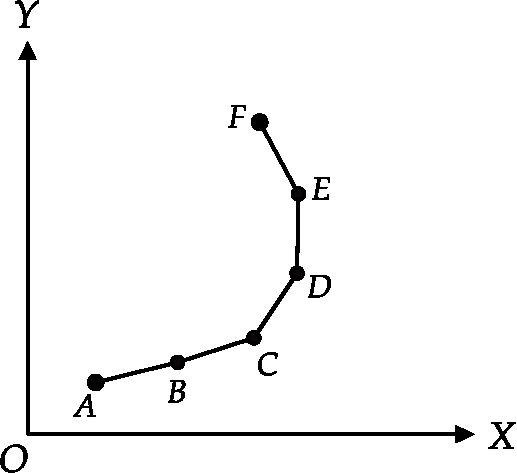
\includegraphics[width=0.25\textwidth]{03-crop}
	\end{center}
	\caption{Geometrical meaning of Differential equation}
\end{wrapfigure}
The solution of every  first order first degree differential equations represent a family of curves.
\\\\Let, $f\left(x, y, \frac{d y}{d x}\right)=0$\quad  represents a differential equation of  first order and first degree.\\\\
Taking $A\left(x_{0}, y_{0}\right)$ as an initial point,we
can find $\frac{d y}{d x}$ at $A\left(x_{0}, y_{0}\right)$. And with the help of that we can draw the tangent at the point $A$.\\\\
On the tangent line take a neighbouring point $B\left(x_{1}, y_{1}\right)$. Find $\frac{d y}{d x}$ at the point $B\left(x_{1}, y_{1}\right)$and draw the tangent at $B$. And in this way draw another tangent at the point $C$ on the tangent line $B$ . Similarly draw, some more tangents by taking the neighbouring points on them. Again we take another starting point $A^{\prime}\left(x_{0}^{\prime}, y_{0}^{\prime}\right)$. We can draw another curve starting from
$A^{\prime} .$ In this way we can draw a number of curves. They form a smooth curve. \\
That is the given difrential equation represents a family of curves.

\section{Solution of a differential equation}
A solution of a differential equation is any relation
between variables which is free of derivatives and which
satisfies the differential equation.\\\\
\textbf{General solution:}\\ A general solution is the solution in which the number
of arbitrary constants and the order of the differential
equation are same.\\\\
\textbf{Particular solution:}\\ A particular solution is the solution which can be
obtained by giving particular values to arbitrary constants of general solution.

\section{Solution of First order differential equations}
The solutions of first order differential equations are obtained by various methods,
\section{ Method of seperation of variables}
If all functions of $x$ and $d x$ can be arranged on one side and $y$ and $d y$ on the other side, then the variables are separable. The solution of this equation is found by integrating the functions of $x$ and $y$.
$$f(x) d x=g(y) d y\Longrightarrow
\int f(x) d x=\int g(y) d y+C
$$
\textbf{\large Method of solving:}
\begin{enumerate}
	\item  Separate the variables as $f(x) d x=g(y) dy$.
    \item Integrate both sides as $\int f(x) d x=\int g(y) d y$.
    \item  Add an arbitrary constant $C$ on R.H.S.
\end{enumerate}
\begin{exercise}
Solve	$\cos (x+y) d y=d x$
\end{exercise}
\begin{answer}[H]
	\begin{align*}
		\cos (x+y) d y&=d x \\
		\frac{d y}{d x}&=\sec (x+y)\\
		\text{  Let, }x+y&=z\\
		\text{  Then, }1+\frac{d y}{d x}=\frac{d z}{d x} \quad & \Rightarrow \quad \frac{d y}{d x}=\frac{d z}{d x}-1 \\
		\frac{d z}{d x}-1=\sec z \quad &\Rightarrow \quad  \frac{d z}{d x}=1+\sec z\\
		\text{Separating the variables, we get, }\\\frac{d z}{1+\sec z}&=d x\\
		\text{On integrating,}\\
		\int \frac{\cos z}{\cos z+1} d z&=\int d x\\
		\int\left[1-\frac{1}{\cos z+1}\right] d z&=x+C \\
		\int\left[ 1-\frac{1}{2 \cos ^{2} \frac{z}{2}-1+1}\right]  d z&=x+C \\
		\int\left(1-\frac{1}{2} \sec ^{2} \frac{z}{2}\right) d z&=x+C\\
		\int\left(1-\frac{1}{2} \sec ^{2} \frac{z}{2}\right) d z&=x+C\\
		z-\tan \frac{z}{2}&=x+C  \\
		x+y-\tan \frac{x+y}{2}&=x+C\\
		 y-\tan \frac{x+y}{2}&=C 
	\end{align*}
\end{answer}
\begin{exercise}
	Solve $e^{d y / d x}=(x+1) ;$ given $y=3$ at $x=0$
\end{exercise}
\begin{answer}
	Taking log of both sides we get, 
	\begin{align*}
		\frac{d y}{d x}=\ln (x+1)\quad &\Rightarrow \quad d y=\ln (x+1) d x\\\text{on integration }, \\\int d y=\int 1 \cdot \ln (x+1) d x \quad &\Rightarrow \quad y=x \ln (x+1)-\int \frac{x}{(x+1)} d x+C\\
		y&=x \ln (x+1)-\int \frac{(x+1)-1}{(x+1)} d x+C\\ y&=x \ln (x+1)-\int \frac{(x+1)}{(x+1)} d x+\int \frac{1}{(x+1)} d x+C\\&=x \ln (x+1)-x+\ln (x+1)+C\\y&=(x+1) \ln (x+1)-x+C\\\text{Given: at,}\ x&=0 \quad y=3 \Rightarrow \quad C=3\\
		\text{Therefore,}\ y&=(x+1) \ln (x+1)-x+3
	\end{align*}
	
\end{answer}
\section{Solution of Homogeneous differential equation}
Homogeneous equations are of the form,
$$
\frac{d y}{d x}=\frac{f(x, y)}{g(x, y)}
$$
Where $f(x, y)$ and $g(x, y)$ are homogeneous functions of the same degree in $x$ and $y$. Homogeneous functions are those in which all the terms are of $n^{th}$  degree.\\\\ 
\textbf{\large Method of solving}
\begin{enumerate}
	\item  Put, $y=v x,$ then $\frac{d y}{d x}=v+x \frac{d y}{d x}$.
	\item  Separate $v$ and $x$ and then integrate.\\\\
	$
	\begin{aligned}
	 \frac{d y}{d x}&=f(y / x) \\
	\Rightarrow  \hspace{1.1cm}y / x&=v \\
	\Rightarrow \hspace{0.3cm}\frac{d v}{f(v)-v}&=\frac{d x}{x} \\
	\Rightarrow  \int \frac{d v}{f(v)-v}&=\log x+C 
	\end{aligned}
	$
\end{enumerate}
\begin{exercise}
	Solve the differential equation $\left(x^{2}-y^{2}\right) d x+2 x y$ $d y=0,$ given that $y=1$ when $x=1$
\end{exercise}
\begin{answer}

	\begin{alignat*}{2}
		\left(x^{2}-y^{2}\right) d x+2 x y d y&=0\\
			\left(x^{2}-y^{2}\right) d x&=-2 x y d y \\
			\frac{d y}{d x}=-\frac{x^{2}-y^{2}}{2 x y}&=\frac{y^{2}-x^{2}}{2 x y}\\
			\text{Putting  } y=v x  \quad &\text{and} \quad \frac{d y}{d x}=v+x \frac{d v}{d x}\\
			\text{ We get}
			\quad v+x \frac{d v}{d x}&=\frac{v^{2} x^{2}-x^{2}}{2 x \cdot v x}\\
			\Rightarrow \hspace{2cm}\quad v+x \frac{d v}{d x}&=\frac{v^{2}-1}{2 v}\\
			\Rightarrow\hspace{2.7cm} x \cdot \frac{d v}{d x}&=\frac{v^{2}-1}{2 v}-v\\&=\frac{v^{2}-1-2 v^{2}}{2 v}\\&=-\left[\frac{v^{2}+1}{2 v}\right]\\
			\Rightarrow \hspace{1.5cm}\quad \frac{2 v}{v^{2}+1} \cdot d v&=-\frac{d x}{x}, \quad x \neq 0\\
			\Rightarrow \hspace{1.1cm}\quad \int \frac{2 v}{v^{2}+1} \cdot d v&=-\int \frac{d x}{x}\\
			\Rightarrow \hspace{1.3cm}\quad \log \left(v^{2}+1\right)&=-\log |x|+c\\
			\Rightarrow \quad \log \left(v^{2}+1\right)+\log |x|&=\log c\\
			\Rightarrow \hspace{1.5cm}\quad\left(v^{2}+1\right)|x|&=c\\
			\text{Now, putting }v&=y / x\\
			\left(y^{2} / x^{2}+1\right)|x|&=c \\
			\Rightarrow \left(x^{2}+y^{2}\right)&=c|x|\\\text{	Which is similar to } x=1 \quad \text{and} \quad y=1, \text{we get,}c&=2\\\text{Putting value of} \quad c&=2 ,\text{We get}\\x^{2}+y^{2}&=2 x \text { or } x^{2}+y^{2}=2(-x)\\x=1 &\quad \text{and}\quad y=1 \\\text{Do not satisfy}\quad x^{2}+y^{2}&=2(-x) \\\text{Hence,}\quad x^{2}+y^{2}&=2 x \quad \text{is the required solution.}
	\end{alignat*}
\end{answer}

\subsection{Equations reducible to homogeneuos form}
Let a differential equation be,
$$
\frac{d y}{d x}=\frac{a x+b y+c}{A x+B y+C}
$$
\textbf{Type-1}\\

\begin{align*}
\text{If, in the above equation,}\quad\frac{a}{A}&\neq\frac{b}{B}\\\text{Then we can substitute}\quad x=X+h\quad&,\quad y=Y+k,\text{($h, k$ being constants)}\\
\text{The given differential equation reduces to}\\
\frac{d Y}{d X}&=\frac{a(X+h)+b(Y+k)+c}{A(X+h)+B(Y+k)+C}\\&=\frac{a X+b Y+a h+b k+c}{A X+B Y+A h+B k+C}\\
\text{Choose $h, k$ so that} \quad a h+b k+c&=0\\
A h+K k+C&=0\\
\text{Then the given equation becomes homogeneous}\\\frac{d Y}{d X}&=\frac{a X+b Y}{A X+B Y}
\end{align*}
\textbf{Type-2}\\
\begin{align*}
\text{If}\ \frac{a}{A}&=\frac{b}{B},\\
\text{Then the value of $h, k$ will not be finite.}\\
\frac{a}{A}&=\frac{b}{B}=\frac{1}{m}\\
A=a m\quad, \quad B&=b \mathrm{~m}\\
\text{The given equation becomes}\quad\frac{d y}{d x}&=\frac{a x+b y+c}{m(a x+b y)+C}
\end{align*}
 Now put $a x+b y=z$ and apply the method of variables separable.
 \begin{exercise}
 	Solve $(x+2 y)(d x-d y)=d x+d y$
 \end{exercise}
\begin{answer}
	\begin{align*}
	(x+2 y)(d x-d y)&=d x+d y \\\Rightarrow(x+2 y-1) d x-(x+2 y+1) d y&=0\\
	\Rightarrow  \frac{d y}{d x}&=\frac{x+2 y-1}{x+2 y+1}\\
	\text { Let } x+2 y&=z \\ 1+2 \frac{d y}{d x}&=\frac{d z}{d x} \\ \frac{d z}{d x}&=\frac{3 z-1}{z+1}\quad  (\text{Since, $ \frac{d y}{d x}=\frac{x+2 y-1}{x+2 y+1}$})\\
	\int \frac{z+1}{3 z-1} dz &=\int dx\\
	\text{L.H.L}&=\int \frac{z+1}{3 z-1} dz\\
	\intertext{multiply numerator and denominator by 3, we get, }
		\text{L.H.L}&=\int \frac{1}{3} \frac{(3z+3)}{(3 z-1)} dz\\
		&=\int \frac{1}{3} \frac{(3z-1+4)}{(3 z-1)} dz\\
		&=\int \frac{1}{3} \frac{(3z-1)+4}{(3 z-1)} dz\\
		&=\int \frac{1}{3}\left\lbrace  \frac{(3z-1)}{(3 z-1)}+ \frac{4}{(3 z-1)}\right\rbrace dz\\
		&=\int \left\lbrace  \frac{1}{3}+  \frac{1}{3} \frac{4}{(3 z-1)}\right\rbrace dz\\
		&=\int \left\lbrace  \frac{1}{3}+  \frac{4}{9} \frac{1}{(3 z-1)}\right\rbrace dz\\
		&=\frac{1}{3} z+\frac{4}{9} \ln (3 z-1)+c
		\intertext{Then,}
		\int \frac{z+1}{3 z-1} dz &=\int dx \Rightarrow	\quad 
		\frac{1}{3} (x+2y)+\frac{4}{9} \ln (3 x+6 y-1)=2x+c\\
		3 x-3 y+a&=2 \ln (3 x+6 y-1)\\
		4 \ln (3 x+6 y-1)&=(6 x-6y)+c\\
	2 \ln (3 x+6 y-1)&=(3 x-3y)+c\\
\end{align*}
\end{answer}
\section{Linear equation of first order}
If a differential equation has its dependent variables and its derivatives occur in the first degree and are not multiplied together, then the equation is said to be linear. The standard equation of a linear equation of first order is given as
$$
\frac{d y}{d x}+P y=Q
$$
Where $P$ and $Q$ are functions of $x$.

\begin{align*}
\text { Integrating factor }&=(\text { I.F. })=e^{\int P \cdot d x} \\
\Rightarrow y \cdot e^{\int P \cdot d x}&=\int Q \cdot e^{\int P \cdot d x} d x+C \\
\Rightarrow \hspace{0.3cm}y(\mathrm{I.F.})&=\int Q(\mathrm{I.F.}) d x+C\\
\end{align*}

\begin{exercise}
	Solve the differential equation $\frac{d y}{d x}-\frac{y}{x}=2 x^{2}, x>0$.
\end{exercise}
\begin{answer}
	we know,
	
	\begin{align*}
		\frac{d y}{d x}+\left(\frac{-1}{x}\right) y &=2 x^{2}\\
		\frac{d y}{d x}+P y=Q, \text { where } P &=-\frac{1}{x} \text { and } Q=2 x^{2}\\
		I.F&=e^{\int P \cdot d x}=e^{\int-1 / x \cdot d x}\\&=e^{-\log x}=e^{\log x^{-1}}=x^{-1}=\frac{1}{x}\\
		\text{Multiplying both sides with $I.F$, we get}\\\frac{1}{x} \cdot \frac{d y}{d x}-\frac{1}{x^{2}} \cdot y&=2 x\\
		\text{Integrating both sides w.r.t. $x,$ we get}\\y \cdot\left(\frac{1}{x}\right)&=\int 2 x \cdot d x+C \\
		\Rightarrow \quad y \cdot \frac{1}{x}&=x^{2}+C\\\Rightarrow\hspace{0.9cm} y&=x^{3}+C x, x>0 \quad \text{is the required solution.}
	\end{align*}
\end{answer}
\subsection{Equations reducible to linear form}
The differential equation of the form,
$$\frac{dy}{dx}+p(x)y=f(x)y^{n}$$is called the Bernoulli's equation or equation reducible to linear form.
It can be done by dividing by $y^{n}$ and substituting $\frac{1}{y^{n-1}}=z$
\begin{alignat*}{2}
&\frac{1}{y^{n}} \frac{d y}{d x}+\frac{1}{y^{n-1}} P&&=Q\\&\text{Put}\quad \frac{1}{y^{n-1}}&&=z\\&\frac{(1-n)}{y^{n}} \frac{d y}{d x}&&=\frac{d z}{d x} \\ &\Rightarrow \quad \frac{1}{y^{n}} \frac{d y}{d x}&&=\frac{d z}{1-n}\\
&\frac{1}{1-n} \frac{d z}{d x}+P z&&=Q \quad \text{or}\\& \frac{d z}{d x}+P(1-n) z&&=Q(1-n)
\end{alignat*}
Which is a linear equation and can be solved easily.
\begin{exercise}
	Solve $\frac{d y}{d x}+x y=x^{3} y^{3}$
\end{exercise}
\begin{answer}We have,
	\begin{align*}
\frac{d y}{d x}+x y&=x^{3} y^{3}\\
\frac{1}{y^{3}} \frac{d y}{d x}+\frac{x}{y^{2}}&=x^{3}\\
	\text{putting}\quad \frac{1}{y^{2}}&=z \\\Rightarrow \quad \frac{-2}{y^{3}} \frac{d y}{d x}&=\frac{d z}{d x} \quad \Rightarrow \quad \frac{1}{y^{3}} \frac{d y}{d x}=\frac{-1}{2} \frac{d z}{d x}\\\therefore \quad-\frac{1}{2} \frac{d z}{d x}+x z&=x^{3} \qquad\Rightarrow \quad \frac{d z}{d x}-2 x z=-2 x^{3}\\
	\mathrm{\therefore I.F.}=e^{-\int 2 x d x}&=e^{-x^{2}}\\
	z e^{-x^{2}}&=-2 \int x^{3} e^{-x^{2}} d x\\
	\text{Let}\quad  -x^{2}&=t \Rightarrow-2 x d x=d t\\
	z e^{-x^{2}}&=\int t e^{t} d t=t e^{t}-e^{t}+c\\
	\text{put}\quad z=y^{-2} \text{and}\quad t=-x^{2}\\
	\therefore \frac{e^{-x^{2}}}{y^{2}}&=-x^{2} e^{-x^{2}}-e^{-x^{2}}+c\\
	\frac{1}{y^{2}}&=-x^{2}-1+C e^{x^{2}}
	\end{align*}
\end{answer}
\section{Exact differential equations}
A differential equation of the form , $Mdx+Ndy=0$ is said to be  exact if it satisfy the following condition,$$\frac{\partial \boldsymbol{M}}{\partial \boldsymbol{y}}=\frac{\partial N}{\partial \boldsymbol{x}}$$
$\frac{\partial M}{\partial \boldsymbol{y}}\quad-\quad$Differential co-efficient of $M$ with respect to $y$ keeping $x$ constant\\
$\frac{\partial N}{\partial \boldsymbol{x}}\quad-\quad$Differential co-efficient of $N$ with respect to $x$, keeping $y$ constant.\\\\
\textbf{\large Method of solving:}\\
\textbf{Step 1:} Integrate $M$ w.r.t. $x$ keeping $y$ constant\\
\textbf{Step 2:} Integrate w.r.t. $y$, only those terms of $N$ which do not contain $x$.\\ \textbf{Step 3:} Result of 1 + Result of 2 = Constant.
\begin{exercise}
	Solve $\left(x^{2}+2 x y\right) d x+\left(x^{2}+y^{2}\right) d y=0$
\end{exercise}
\begin{answer}
	\begin{align*}
	\text{Here,}\quad M=\left(x^{2}+2 x y\right) \quad &\text{and}\quad N=\left(x^{2}+y^{2}\right)\\\Rightarrow \frac{\partial M}{\partial y}&=2 x\\\text{and}\quad
	\frac{\partial N}{\partial x}&=2 x\\
	\text{Hence, the given equation is exact}\\
	\int\left(x^{2}+2 x y\right) d x+\int y^{2} d y&=c\\\frac{x^{3}}{3}+x^{2} y+\frac{y^{3}}{3}&=C\\\text { The solution is: } \\\int\left(x^{2}+2 x y\right) d x+\int y^{2} d y=c=\frac{x^{3}}{43}+x^{2} y+\frac{y^{3}}{3}&=6\end{align*}
\end{answer}
\subsection{Equations reducible to Exact form}
A differential equation which is not exact can be reduced to exact form  by multiplying it by a constant , here the integrating factor.\\
\textbf{Type 1:} If $ \frac{\frac{\partial M}{\partial y}-\frac{\partial N}{\partial x}}{N}\text { is a function of } x \text { alone, say } f(x), \text { then } \mathrm{I.F}=e^{\int f(x) d x}$\\
\textbf{Type 2:} If $\frac{\frac{\partial N}{\partial x}-\frac{\partial M}{\partial y}}{M}$ is a function of $y$ alone, say $f(y),$ then
$
\mathrm{I.F} =e^{\int f(y) d y}
$
\begin{exercise}
	Solve $(2 x \log x-x y) d y+2 y d x=0$
\end{exercise}
\begin{answer}
\begin{align*}
M &=2 y,\quad N=2 x \log x-x y\notag\\
\frac{\partial M}{\partial y}&=2,\quad\frac{\partial N}{\partial x}=2(1+\log x)-y\\
\text { Here, }\notag \\
\quad \frac{\frac{\partial M}{\partial y}-\frac{\partial N}{\partial x}}{N}&=\frac{2-2-2 \log x+y}{2 x \log x-x y}\\&=\frac{-(2 \log x-y)}{x(2 \log x-y)}=-\frac{1}{x}=f(x)\notag\\\text { I.F. }&=e^{\int f(x) d x}=e^{\int-\frac{1}{x} d x}\\&=e^{-\log x}=e^{\log x^{-1}}=x^{-1}=\frac{1}{x}\\
&\text{On multiplying the given differential equation by}  \frac{1}{x}, \text{we get}\\
\frac{2 y}{x} d x+(2 \log x-y) d y&=0 \\ \Rightarrow \quad \int \frac{2 y}{x} d x+\int-y d y&=c \\
\Rightarrow  \qquad\quad 2 y \log x-\frac{1}{2} y^{2}&=c
\end{align*}
\end{answer}
\section{Orthogonal trajectories and Family of curves}
Given a one-parameter family of plane curves, it's orthogonal trajectories are another
one-parameter family of curves, each one of which is perpendicular to all the curves in the
original family. For instance, if the original family consisted of all circles having center at the origin, it's orthogonal trajectories would be all rays (half-lines) starting at the origin.
\begin{definition}
	Two families of curves are such that every curve of either family cuts each curve of the other family at right angles. They are called orthogonal trajectories of each other.
\end{definition}
Orthogonal trajectories arise in different contexts in applications. If the
original family represents the lines of force in a gravitational or electrostatic field, its orthogonal trajectories represent the equipotentials, the curves along which the gravitational or electrostatic potential is constant.
\begin{example}\hspace{1cm}
	\begin{enumerate}
		\item The path of an electric field is perpendicular to equipotential curves.
		\item  In fluid flow, the stream lines and equipotential lines are orthogonal trajectories.
		\item The lines of heat flow is perpendicular to isothermal curves.
	\end{enumerate}
\end{example}
\subsection{Finding orthogonal trajectories to the curve}
Let a family of curves be given by the equation
$$
g(x, y)=C
$$
Where $C$ is a constant. For the given family of curves, we can draw the orthogonal trajectories, that is another family of curves $f(x, y)=C$ that cross the given curves at right angles.
\subsubsection{Method of solving}
\textbf{Family of curves given ,then to find orthogonal trajectories.}
\begin{enumerate}
	\item  By differentiating the equation of curves find the differential equations in the form $f\left(x, y, \frac{d y}{d x}\right)=0$
	\item  Replace $\frac{d y}{d x}$ by $-\frac{d x}{d y}$\\ ($ m_{1}m_{2}=-1$, where,$m_{1}$=given family,$m_{2}$=orthogonal  family)
	\item  Solve the differential equation of the orthogonal trajectories i.e., $f\left(x, y,-\frac{d x}{d y}\right)=0$
\end{enumerate}
\textbf{Orthogonal trajectories given , then to find Family of curves .}
\begin{enumerate}
	\item Solve the differential equation of the orthogonal trajectory $f\left(x, y,\frac{d x}{d y}\right)=0$ using appropriate method.
\end{enumerate}
\begin{note}
	\textbf{Self-orthogonal:}. If the family of orthogonal trajectory is the same as the given family of curves,then it's called self orthogonal.
\end{note}
\begin{exercise}
	 Find the orthogonal trajectories of the family of straight lines  $y=C x,$  where  $C$  is a parameter.
\end{exercise}
\begin{answer}
	\begin{align*}
	\text{we have,}\quad y&=C x\\
	\text{differentiating the given equation we get}\\
	dy&=cdx\\
	dy&=\frac{y}{x}dx\quad(\because c=\frac{y}{x})\\
	\frac{dy}{dx}=\frac{y}{x}\\
	{\frac{dy}{dx}}_{(ortho)}&=\frac{-x}{y}\\
	\text{ using variable separable method}\\
	(-xdx&=ydy)\\
	\int-xdx&=\int ydy\\
	-\frac{x^{2}}{2}&=\frac{y^{2}}{2}+C\\
		\frac{x^{2}}{2}+\frac{y^{2}}{2}&=C\\
		x^{2}+y^{2}&=2C\Longrightarrow \text{Represents the family of circles}
	\end{align*}
\end{answer}
\begin{exercise}
	Find the family of curves of the given trajectory,	$\frac{dy}{dx}=\frac{x}{y}$
\end{exercise}
\begin{answer}
\begin{align*}
\text{given},\frac{dy}{dx}&=\frac{x}{y}\\
\text{using variable seperable method, we get}\\
\int xdx&=\int ydy\\
\frac{x^{2}}{2}&=\frac{y^{2}}{2}+C\\
\frac{x^{2}}{2}-\frac{y^{2}}{2}&=C\\
x^{2}-y^{2}&=2C\Longrightarrow \text{family of hyperbolas}
\end{align*}
\end{answer}
\section{Second order differential equations}
\subsection{Linear differential equation}
If the degree of the dependent variable and all derivatives is one, such differential equations are called linear differential equations.
\begin{example}\hspace{0.5cm}
	\begin{enumerate}
		\item $2\frac{d^{2} y}{d x^{2}}+3\frac{d y}{d x}+4 y=x^{2}+x+1$
		\item $ \frac{d^{2} x}{d x^{2}}-\frac{d y}{d x}-3 y=x$
		\item $2 \frac{d^{2} x}{d t^{2}}-\frac{d x}{d t}-3 x=f(t)$
	\end{enumerate}
\end{example}
\subsection{Non-Linear differential equation}
If the degree of the dependent variable and / or its derivatives are of greater than 1 such differential equations are called non-linear differential equations.
\begin{example}\hspace{0.5cm}
	\begin{enumerate}
		\item $\frac{d^{2} y}{d x^{2}}+\frac{d y}{d x}+y^{2}=\sin x$
		\item  $\frac{d^{2} y}{d x^{2}}+2\left(\frac{d y}{d x}\right)^{2}+y^{2}=e^{x}$
		\item  $\left(\frac{d^{2} x}{d t^{2}}\right)^{2}+\frac{d x}{d t}+x=f(t)$
	\end{enumerate}
\end{example}
\subsection{Homogeneous differential equation}
A differential equation of the form
$y^{\prime \prime}+P(x) y^{\prime}+Q(x) y=F(x)$, is said to be  homogeneous if $F(x)= 0$
\begin{example}
	\hspace{0.5cm}
	\begin{enumerate}
		\item 	$\frac{d^{2} y}{d x^{2}}-6 \frac{d y}{d x}+13 y=0$
		\item $\frac{d^{2} y}{d x^{2}}+2\left(\frac{d y}{d x}\right)^{2}+y^{2}=0$
	\end{enumerate}

\end{example}
\subsection{Nonhomogeneous differential eqaution} A differential equation of the form
$y^{\prime \prime}+P(x) y^{\prime}+Q(x) y=F(x)$, is said to be  non-homogeneous if $F(x)\neq 0$
\begin{example}
\hspace{0.5cm}
\begin{enumerate}
	\item 	$\frac{d^{2} y}{d x^{2}}-6 \frac{d y}{d x}+ y=x^{2}+2$
	\item $\frac{d^{2} y}{d x^{2}}+2\left(\frac{d y}{d x}\right)^{2}+y^{2}=e^{x}$
\end{enumerate}
\end{example}
\section{Linear independance and dependance of solutions}
Two solutions of a differential equation, $ y_{1}(x)$ and $ y_{2}(x)$ are said to be linearly independant if \\$$Ay_{1}(x)+By_{2}(x)\neq 0 $$ given, $ A\neq0 \quad\text{and}\quad B\neq0$
\subsection{Wronskian}
A first-order homogeneous ODE has only one linearly independent solution. This is meant in the following sense. "If two solutions are linearly dependent, by definition they satisfy $a y_{1}(x)+b y_{2}(x)=0$ with nonzero constants $a, b$ for all values of $x$". If the only solution of this linear relation is $a=0=b$, then our solutions $y_{1}$ and $y_{2}$ are said to be linearly independent.
\\To prove this theorem, suppose $y_{1}, y_{2}$ both solve the homogeneous ODE. Then,
\begin{equation*}
\frac{y_{1}^{\prime}}{y_{1}}=-p(x)=\frac{y_{2}^{\prime}}{y_{2}} \quad \Rightarrow \quad W(x) \equiv y_{1}^{\prime} y_{2}-y_{1} y_{2}^{\prime} \equiv 0
\end{equation*}
The functional determinant $W$ is called the \textbf{Wronskian of the pair $y_{1}$, $y_{2}$}. We now show that $W \equiv 0$ is the condition for them to be linearly dependent. Assuming linear dependence, that is.
\begin{equation*}
a y_{1}(x)+b y_{2}(x)=0
\end{equation*}
In matrix form, the Wronskian of two functions $y_{1}(x)$ and $y_{2}(x)$ is given by,
\begin{equation}
W\left(y_{1}, y_{2}, x\right)=\left|\begin{array}{ll}
y_{1}(x) & y_{2}(x) \\
y_{1}^{\prime}(x) & y_{2}^{\prime}(x)
\end{array}\right|=y_{1}(x) y_{2}^{\prime}(x)-y_{1}^{\prime}(x) y_{2}(x)
\end{equation}
\begin{enumerate}
	\item If $W\left(y_{1}, y_{2}, x\right)=0,$ then $y_{1}(x)$ and $y_{2}(x)$ are linearly dependent.
	\item If $W\left(y_{1}, y_{2}, x\right) \neq 0,$ then $y_{1}(x), y_{2}(x)$ are linearly independent.
\end{enumerate}
\begin{note}
	The wronskian of a differential equation can also be written as,
	$$ W(t)=e^{-\int p(x)dx}$$
	\end{note}
\begin{exercise}
Consider two solutions $\mathrm{x}_{1}(\mathrm{t})$ and $\mathrm{x}_{2}(\mathrm{t})$ of the differential equation $\frac{d^{2} x(t)}{d t^{2}}+x(t)=0, t>0$, such that $x_{1}(0)=1,\left.\frac{d x_{1}(t)}{d t}\right|_{t=0}=0, x_{2}(0)=0,\left.\frac{d x_{2}(t)}{d t}\right|_{t=0}=1$. The Wronskian $W(t)=\left|\begin{array}{ll}x_{1}(t) & x_{2}(t) \\ \frac{d x_{1}(t)}{d t} & \frac{d x_{2}(t)}{d t}\end{array}\right|$ at $t=\frac{\pi}{2}$ is,	
\end{exercise}
\begin{answer}
	The wronskian of a differential equation can also be written as,
	\begin{align*}
	W(t)&=e^{-\int p(x)dx}\\
	\text{But here,}\quad  p(x)&=0\\
	\text{Then,} \quad W(t)&=e^{0 \ dx}=1\\
	\text{So,}\quad W(\frac{\pi}{2})&=1
	\end{align*}
\end{answer}
\section{Linear Second Order Differential Equations With Constant Coefficients}
The general form of the linear differential equation of second order is
$$
\frac{d^{2} y}{d x^{2}}+P \frac{d y}{d x}+Q y=R
$$
Where $P$ and $Q$ are constants and $R$ is a function of $x$ or constant.\begin{note}\textbf{Differential operator:}\\
	A differential operator can be represented as,\quad $D=\frac{d}{dx}$
\\Then a differential equation can be written  in terms of differntial operators as,
\begin{align*}
D^{2} y+P D y+Q y&=R \\ \left(D^{2}+P D+Q\right) y&=R\\
\text{Where,}\quad D y&=\frac{d y}{d x}, \ \text{and}\ D^{2} y=\frac{d^{2} y}{d x^{2}}
\end{align*}

$\frac{1}{D}$ stands for the operation of integration.	
\end{note}
\section{Solution of Second order homogeneous differential equation.}

\subsection{Method of solving}
\begin{enumerate}
	\item Let $y=C_{1} e^{m x}$ be the trial solution
	\begin{equation}
	\frac{d^{2} y}{d x^{2}}+P \frac{d y}{d x}+Q y=0\label{eq1}
	\end{equation}
	
	Putting the values of $y,\quad \frac{d y}{d x}$ and $\quad\frac{d^{2} y}{d x^{2}}$ in  \ref{eq1} then,\\ $C_{1} e^{m x}\left(m^{2}+P m+Q\right)=0$
	$\Rightarrow$
	$m^{2}+P m+Q=0 .$ It is called Auxiliary equation.
	\item Solve the auxiliary equation.
	\subsubsection{{Case 1:}}\textbf{ Roots are real and distinct}\\
	If $m_{1}$ and $m_{2}$ are the roots, then the C.F. is
	$$
	y=C_{1} e^{m_{1} x}+C_{2} e^{m_{2} x}
	$$
	\subsubsection{{Case 2:}}\textbf{ Roots are real and  equal}\\
	If both the roots are $m, m$ then the C.F. is
	$$
	y=\left(C_{1}+C_{2} x\right) e^{m x}
	$$
	\subsubsection{{Case 3:}}\textbf{ Roots are Imaginary}\\
	 If the roots are $\alpha \pm i \beta,$ then the solution will be
	$$
	\begin{aligned}
	y &=C_{1} e^{(\alpha+i \beta) x}+C_{2} e^{(\alpha-i \beta) x}=e^{\alpha x} \cdot\left[C_{1} e^{i \beta x}+C_{2} e^{-i \beta x}\right] \\
	&=e^{\alpha x}\left[C_{1}(\cos \beta x+i \sin \beta x)+C_{2}(\cos \beta x-i \sin \beta x)\right] \\
	&=e^{\alpha x}\left[\left(C_{1}+C_{2}\right) \cos \beta x+i\left(C_{1}-C_{2}\right) \sin \beta x\right]\\&=e^{\alpha x}[A \cos \beta x+B \sin \beta x]
	\end{aligned}
	$$
\end{enumerate}
\setlength\extrarowheight{10pt}
\begin{table}[H]
\begin{tabular}{|m{5cm}|m{4cm}|m{4cm}|}
\hline
Roots&Basis of solution&General solution\\\hline
Real and  equal(repeated root $m$)& $e^{m x}$ and $xe^{m x}$&$
y=\left(C_{1}+C_{2} x\right) e^{m x}
$\\\hline
Real and  distinct($m_{1}$ , $m_{2}$)& $e^{m_{1} x}$ ,$\quad e^{m_{2} x}$ &$
y=C_{1} e^{m_{1} x}+C_{2} e^{m_{2} x}
$\\\hline
Imaginary roots ($\alpha \pm i \beta$)&$ e^{(\alpha+i \beta) x}, e^{(\alpha-i \beta) x}$&$e^{\alpha x}[A \cos \beta x+B \sin \beta x]$\\\hline

\end{tabular}
\caption{Roots of homogeneous second order DE}
\end{table}
\begin{exercise}
	Solve $\frac{d^{2} y}{d x^{2}}-8 \frac{d y}{d x}+15 y=0$.
\end{exercise}
\begin{answer}
	\begin{align*}
	\text{Given equation can be written as,}\\
	\left(D^{2}-8 D+15\right) y&=0\\
	\text{Here auxiliary equation is,}\\ m^{2}-8 m+15&=0\\
	(m-3)(m-5)&=0 \quad \therefore m=3,5\\\text{Hence, the required solution is,}\\
	y&=C_{1} e^{3 x}+C_{2} e^{5 x}
	\end{align*}
\end{answer}
\begin{exercise}
	Solve the differential equation:
	$
	\frac{d^{2} y}{d x^{2}}+6 \frac{d y}{d x}+9 y=0
	$
\end{exercise}
\begin{answer}
We have
\begin{align*}
\frac{d^{2} y}{d x^{2}}+6 \frac{d y}{d x}+9 y&=0 \\
\Rightarrow \left(D^{2}+6 D+9\right) y&=0\\
\text{Auxiliary equation is}\quad D^{2}+6 D+9&=0\\
\Rightarrow \quad(D+3)^{2}&=0 \Rightarrow D=-3,-3\\
\text{the solution, y}&=\left(c_{1}+c_{2} x\right) e^{-3 x}
\end{align*}
\end{answer}
\begin{exercise}
	Solve $\left(D^{3}-1\right) y=0$
\end{exercise}
\begin{answer}
	\begin{align*}
	\text{we have,}\left(D^{3}-1\right) y&=0\\
	\text{The characteristic equation is,}\\
	m^{3}-1&=0 \Rightarrow m=1, \frac{-1 \pm \sqrt{3 i}}{2}\\\text { y }&=A e^{x}+e^{-x / 2} \cdot\left[B \cos \frac{\sqrt{3}}{2} x+C \sin \frac{\sqrt{3}}{2} x\right]
	\end{align*}
\end{answer}
\section{Solution of Second order nonhomogeneous differential equation.}
The solution of a differential equation of the form,$$\frac{d^{2} y}{d x^{2}}+P \frac{d y}{d x}+Q y=R$$ consists of two parts,a complementary function and a particular integral.
\\Complete Solution = Complementary Function + Particular Integral
\begin{center}
	\framebox{
		\parbox[t][0.75cm]{4cm}{
			
			\addvspace{0.2cm} \centering 
			
			{y}\quad=\quad{C . F }\quad+\quad{P . I}} }
\end{center}
\subsubsection{Finding complementary function}
Complementary function is the solution obtained by solving the equation replacing R.H.S by 0.Same as that explained in finding solution to homogeneous differential equations.
\subsubsection{Finding Particular solution}
Particular integral (P.I) depends on the form of $R(x)$\\
If the differential equation is of the form,$$\left(D^{n}+k_{1} D^{n-1}+k_{2} D^{n-2}+\cdots+k_{n}\right) y=R(x)$$
\\Then the particular integral of the equation is given by,
$$
\text { P.I. }=\frac{1}{D^{n}+k_{1} D^{n-1}+k_{2} D^{n-2}+\cdots+k_{n}} R(x)
$$
The following cases arise for particular integrals:
\begin{enumerate}
	\item When $X=e^{a x},$ then
	$$
	\begin{aligned}
	\text { P.I. } &=\frac{1}{f(D)} e^{a x} \\
	&=\frac{1}{f(a)} e^{a x},\quad \text { If }\ f(a) \neq 0 \\
	\text { If } f(a)=0, \text { then } \\
	\text { P.I. } &=\frac{x}{f^{\prime}(a)} e^{a x}, \quad \text { If }\ f^{\prime}(a) \neq 0
	\end{aligned}
	$$
	If $f^{\prime}(a)=0,$ then
	$$
	\text { P.I. }=\frac{x^{2}}{f^{\prime \prime}(a)} e^{a x}, \quad \text { If }\ f^{\prime \prime}(a) \neq 0
	$$
	\item  When $X=\sin a x,$ then
	$$
	\begin{array}{c}
	\text { P.I. }=\frac{1}{f\left(D^{2}\right)} \sin a x \\
	=\frac{1}{f\left(-a^{2}\right)} \sin a x, \text { if } f\left(-a^{2}\right) \neq 0
	\end{array}
	$$
	\item When $X=\cos a x,$ then
	$$
	\begin{aligned}
	\text { P.I. } &=\frac{1}{f\left(D^{2}\right)} \cos a x \\
	&=\frac{1}{f\left(-a^{2}\right)} \cos a x, \text { if } f\left(-a^{2}\right) \neq 0
	\end{aligned}
	$$
	\item  When $X=x^{m}$, then
	$$
	\text { P.I. }=\frac{1}{f(D)} x^{m}=[f(D)]^{-1} x^{m}
	$$
	Expansion of $[f(D)]^{-1}$ is to be carried up to the term $D^{m}$ because $(m+1)^{\text {th }}$ and higher derivatives of $x^{m}$ are zero.
	\item When $X=e^{a x} v(x)$, then
	$$
	\begin{array}{l}
	\text { P.I. }=\frac{1}{f(D)} e^{a x} v(x) \\
	\text { P.I. }=e^{a x} \frac{1}{f(D+a)} v(x)
	\end{array}
	$$
	\item When $X=x v(x)$, then
	\begin{align*}
	\text { P.I. }&=\frac{1}{f(D)} x v(x)\\&=\left[x-\frac{f^{\prime}(D)}{f(D)}\right] \cdot \frac{1}{f(D)} v(x)
	\end{align*}
\end{enumerate}
\begin{exercise}
	Solve the differential equation:
	$$
	\frac{d^{2} y}{d x^{2}}+6 \frac{d y}{d x}+9 y=5 e^{3 x}
	$$
\end{exercise}
\begin{answer}
	We have
	\begin{align*}
	\frac{d^{2} y}{d x^{2}}+6 \frac{d y}{d x}+9 y&=5 e^{3 x} \\
	 \left(D^{2}+6 D+9\right) y&=5 e^{3 x}\\
	\text{Auxiliary equation is}\quad D^{2}+6 D+9&=0\\
(D+3)^{2}&=0 \Rightarrow D=-3,-3\\
	\text{The solution, y}&=\left(c_{1}+c_{2} x\right) e^{-3 x}\\
	\text { Particular integral } &=\frac{1}{D^{2}+6 D+9} \cdot 5 e^{3 x} \\
	&=\frac{5 e^{3 x}}{(3)^{2}+6(3)+9}=\frac{5 e^{3 x}}{36}\\
	\text{The complete solution is given by} y&=\mathrm{C} . \mathrm{F} .+\mathrm{P} . \mathrm{I}\\
 y&=\left(c_{1}+c_{2} x\right) e^{-3 x}+\frac{5 e^{3 x}}{36}
	\end{align*}
\end{answer}
\begin{exercise}
	Find the particular integral of the differential equation, $(D^{3}+8)=x^{4}-2x+1$
\end{exercise}
\begin{answer}
	We have,
	\begin{align*}
	(D^{3}+8)&=x^{4}-2x+1\\
	\text{P.I}&=\frac{1}{(D^{3}+8)}(x^{4}-2x+1)\\
	&=\frac{1}{8(1+\frac{D^{3}}{8})}(x^{4}-2x+1)\\
	&=\frac{[1+\frac{D^{3}}{8}]^{-1} }{8}(x^{4}-2x+1)
	\intertext{Using Binomial expansion on $[1+\frac{D^{3}}{8}]^{-1}$ we get,}
	[1+\frac{D^{3}}{8}]^{-1}&=[1-\frac{D^{3}}{8}+\cdots]
	\intertext{Higher terms in the expansion can be ommitted since , here the  highest power of $x$ is $4$ ($R(x)=x^{4}-2x+1$).}
	\text{Then,}\ \text{P.I}&=\frac{1}{8}[1-\frac{D^{3}}{8}](x^{4}-2x+1)\\
	&=\frac{1}{8}\left[ (x^{4}-2x+1)-\frac{D^{3} (x^{4}-2x+1)}{8}\right] \\
	&=\frac{1}{8}\left[ (x^{4}-2x+1)-\frac{24x}{8}\right] \\
	&=\frac{1}{8}\left[ (x^{4}-2x+1)-3x\right] \\
	&=\frac{1}{8}\left[ (x^{4}-x+1)\right]
	\end{align*}
\end{answer}
\section{Euler - Cauchy Differential equation}
 A homogeneous differential equation of the form,
 \begin{equation}
 a_{n} x^{n} \frac{d^{n} y}{d x^{n}}+a_{(n-1)} x^{(n-1)} \frac{d^{(n-1)} y}{d x^{(n-1)}}+\cdots \cdots+a_{2} x^{2} \frac{d^{2} y}{d x^{2}}+a_{1} x \frac{d y}{d x}+a_{0} y=\mathrm{Q(x)}
 \end{equation}
 Where, $a_{0},a_{1},a_{2}\cdots a_{n} $ are constants is called a Euler - Cauchy differential equation.
 \begin{align*}
 \text{Put,} \ \mathrm{x}&=\mathrm{e}^{z} \Rightarrow \log \mathrm{x}=\mathrm{z} \Rightarrow \frac{1}{x}=\frac{d z}{d x}\\
 \frac{d y}{d x}&=\frac{d y}{d x} \cdot \frac{d z}{d x}\\&=\frac{1}{x} \frac{d y}{d z} \\ \mathrm{x} \frac{d y}{d x}&=\frac{d y}{d z}\\
 \frac{d^{2} y}{d x^{2}}&=\frac{d}{d x}\left(\frac{d y}{d x}\right)\\&=-\frac{1}{x^{2}} \frac{d y}{d z}+\frac{1}{x} \frac{d^{2} y}{d z^{2}}\left(\frac{d z}{d x}\right)\\&=-\frac{1}{x^{2}} \frac{d y}{d z}+\frac{1}{x^{2}} \frac{d^{2} y}{d z^{2}} \\ x^{2} \frac{d y}{d x^{2}}&=-\frac{d y}{d z}+\frac{d^{2} y}{d z^{2}}
\intertext{ Then neglecting the higher orders , the given equation becomes,}
  a_{2} \frac{d^{2} y}{d z^{2}}+\left(a_{1}-a_{2}\right) \frac{d y}{d z}+a_{0} y&=\mathrm{Q} \\
  \intertext{Linear second order non-homogeneous differential equation}
 \end{align*}
 \begin{exercise}
 	$x^{2} \frac{d^{2} y}{d x^{2}}+2 x \frac{d y}{d x}-20 y=(x+1)^{2}$
 \end{exercise}
\begin{answer}
	\begin{align*}
	x&=e^{z} \\ \log x&=z \Rightarrow \frac{1}{x}=\frac{d z}{d x}\\
	\text{Let,}\ x \frac{d y}{d x}&=\frac{d y}{d z}\\
	\text{and,} x^{2} \frac{d^{2} y}{d x^{2}}&=\frac{d^{2} y}{d z^{2}}-\frac{d y}{d z}\\
	\text{Then we get,} \frac{d^{2} y}{d z^{2}}+\frac{d y}{d z}-20 y&=\left(e^{z}+1\right)^{2}\\
	\text{C.F.} &=c_{1} e^{4 z}+c_{2} e^{-5 z}\\&=c_{1} x^{4}+c_{2} x^{-5}\\
	\text{P . I .}&=\frac{1}{D^{2}+D-20}\left(e^{z}+1\right)^{2}\\&=\frac{1}{D^{2}+D-20}\left(e^{2 z}+2 e^{z}+1\right)\\&=-\frac{1}{14} e^{2 z}-\frac{1}{9} e^{z}-\frac{1}{20}\\
	\text{Total solution} \ y&=c_{1} x^{4}+c_{2} x^{-5}-\frac{1}{14} x^{2}-\frac{1}{9} x-\frac{1}{20}
	\end{align*}
\end{answer}

%\section{Singular Points}
%The concept of singular point or singularity (as applied to a differential equation) stems from the ts usefulness in  classifying Ordinary Differential Equations  and  investigating the feasibility of a series solution (Series Solution method will be explained in the next section)
%If we write our second-order homogeneous differential equation (in $y$ ) as,
%\begin{equation}
%y^{\prime \prime}+P(x) y^{\prime}+Q(x) y=0 \label{DE001}
%\end{equation}
%We are ready to define ordinary and singular points. If the functions $P(x)$ and $Q(x)$ remain finite at $x=x_{0}$, point $x=x_{0}$ is an ordinary point. However, if either $P(x)$ or $Q(x)$ (or both) diverges as $x \rightarrow x_{0}$, point $x_{0}$ is a singular point. Using equation \ref{DE001} we may distinguish between two kinds of singular points.
%\begin{enumerate}
%	\item If either $P(x)$ or $Q(x)$ diverges as $x \rightarrow x_{0}$ but $\left(x-x_{0}\right) P(x)$ and $\left(x-x_{0}\right)^{2} Q(x)$ remain finite as $x \rightarrow x_{0}$, then $x=x_{0}$ is called a \textbf{regular}, or \textbf{nonessential, singular point.}
%	\item If $P(x)$ diverges faster than $\frac{1}{\left(x-x_{0}\right)} $ so that $\left(x-x_{0}\right) P(x)$ goes to infinity as $x \rightarrow x_{0}$, or $Q(x)$ diverges faster than $\frac{1}{\left(x-x_{0}\right)} ^{2}$ so that $\left(x-x_{0}\right)^{2} Q(x)$ goes to infinity as $x \rightarrow x_{0}$, then point $x=x_{0}$ is labeled an \textbf{irregular}, or \textbf{essential, singularity}.
%\end{enumerate}
 
\newpage
\begin{abox}
	Problem Set -1
\end{abox}
\begin{enumerate}[label=\color{ocre}\textbf{\arabic*.}]	
	\item Let $x_{1}(t)$ and $x_{2}(t)$ be two linearly independent solutions of the differential equation $\frac{d^{2} x}{d t^{2}}+2 \frac{d x}{d t}+f(t) x=0$ and let $w(t)=x_{1}(t) \frac{d x_{2}(t)}{d t}-x_{2}(t) \frac{d x_{1}(t)}{d t} .$ If $w(0)=1$, then $w(1)$ is given by
	{\exyear{ NET/JRF(DEC-2011)}}
			\begin{tasks}(4)
			\task[\textbf{A.}] 1
			\task[\textbf{B.}] $e^{2}$
			\task[\textbf{C.}]  $1 / e$
			\task[\textbf{D.}] $1 / e^{2}$
		\end{tasks}
\item Let $y(x)$ be a continuous real function in the range 0 and $2 \pi$, satisfying the inhomogeneous differential equation: $\sin x \frac{d^{2} y}{d x^{2}}+\cos x \frac{d y}{d x}=\delta\left(x-\frac{\pi}{2}\right)$ The value of $d y l d x$ at the point $x=\pi / 2$
{\exyear{NET/JRF (JUNE-2012)}}
\begin{tasks}(2)
	\task[\textbf{A.}] Is continuous
	\task[\textbf{B.}] Has a discontinuity of 3
	\task[\textbf{C.}] Has a discontinuity of $1 / 3$
	\task[\textbf{D.}] Has a discontinuity of 1
\end{tasks}
\item The solution of the partial differential equation
$$
\frac{\partial^{2}}{\partial t^{2}} u(x, t)-\frac{\partial^{2}}{\partial x^{2}} u(x, t)=0
$$
satisfying the boundary conditions $u(0, t)=0=u(L, t)$ and initial conditions $u(x, 0)=\sin (\pi x / L)$ and $\left.\frac{\partial}{\partial t} u(x, t)\right|_{t=0}=\sin (2 \pi x / L)$ is
{\exyear{NET/JRF(JUNE-2013)}}
	\begin{tasks}(1)
		\task[\textbf{A.}] $\sin (\pi x / L) \cos (\pi t / L)+\frac{L}{2 \pi} \sin (2 \pi x / L) \cos (2 \pi t / L)$
		\task[\textbf{B.}] $2 \sin (\pi x / L) \cos (\pi t / L)-\sin (\pi x / L) \cos (2 \pi t / L)$
		\task[\textbf{C.}] $\sin (\pi x / L) \cos (2 \pi t / L)+\frac{L}{\pi} \sin (2 \pi x / L) \sin (\pi t / L)$
		\task[\textbf{D.}] $\sin (\pi x / L) \cos (\pi t / L)+\frac{L}{2 \pi} \sin (2 \pi x / L) \sin (2 \pi t / L)$
	\end{tasks}
	\item The solution of the differential equation
	$$
	\frac{d x}{d t}=x^{2}
	$$
	with the initial condition $x(0)=1$ will blow up as $t$ tends to
	{\exyear{NET/JRF(JUNE-2013)}}
	\begin{tasks}(4)
		\task[\textbf{A.}] 1
		\task[\textbf{B.}] 2
		\task[\textbf{C.}] $\frac{1}{2}$
		\task[\textbf{D.}] $\infty$
	\end{tasks}
	\item Consider the differential equation
	$$
	\frac{d^{2} x}{d t^{2}}+2 \frac{d x}{d t}+x=0
	$$
	with the initial conditions $x(0)=0$ and $\dot{x}(0)=1$. The solution $x(t)$ attains its maximum value when $t$ is
	{\exyear{NET/JRF(JUNE-2014)}}
	\begin{tasks}(4)
		\task[\textbf{A.}] $1 / 2$
		\task[\textbf{B.}] 1
		\task[\textbf{C.}] 2
		\task[\textbf{D.}] $\infty$
	\end{tasks}
	\item Consider the differential equation $\frac{d^{2} x}{d t^{2}}-3 \frac{d x}{d t}+2 x=0$. If $x=0$ at $t=0$ and $x=1$ at $t=1$, the value of $x$ at $t=2$ is
	{\exyear{NET/JRF(JUNE-2015)}}
	\begin{tasks}(4)
		\task[\textbf{A.}] $e^{2}+1$
		\task[\textbf{B.}] $e^{2}+e$
		\task[\textbf{C.}] $e+2$
		\task[\textbf{D.}] $2 e$
	\end{tasks}
	\item  If $y=\frac{1}{\tanh (x)}$, then $x$ is
	{\exyear{NET/JRF(DEC-2015)}}
	\begin{tasks}(4)
		\task[\textbf{A.}] $\ln \left(\frac{y+1}{y-1}\right)$
		\task[\textbf{B.}] $\ln \left(\frac{y-1}{y+1}\right)$
		\task[\textbf{C.}]  $\ln \sqrt{\frac{y-1}{y+1}}$
		\task[\textbf{D.}]  $\ln \sqrt{\frac{y+1}{y-1}}$
	\end{tasks}
	\item The solution of the differential equation $\frac{d x}{d t}=2 \sqrt{1-x^{2}}$, with initial condition $x=0$ at $t=0$ is
	{\exyear{NET/JRF(DEC-2015)}}
	\begin{tasks}(2)
		\task[\textbf{A.}] $x=\left\{\begin{array}{ll}\sin 2 t, & 0 \leq t<\frac{\pi}{4} \\ \sinh 2 t, & t \geq \frac{\pi}{4}\end{array}\right.$
		\task[\textbf{B.}] $x=\left\{\begin{array}{cc}\sin 2 t, & 0 \leq t<\frac{\pi}{2} \\ 1, & t \geq \frac{\pi}{2}\end{array}\right.$
		\task[\textbf{C.}] $x=\left\{\begin{array}{cc}\sin 2 t, & 0 \leq t<\frac{\pi}{4} \\ 1, & t \geq \frac{\pi}{4}\end{array}\right.$
		\task[\textbf{D.}] $x=1-\cos 2 t, \quad t \geq 0$
	\end{tasks}
	\item   The function $y(x)$ satisfies the differential equation $x \frac{d y}{d x}+2 y=\frac{\cos \pi x}{x}$. If $y(1)=1$, the value of $y(2)$ is
	{\exyear{NET/JRF(JUNE-2017)}}
	\begin{tasks}(4)
		\task[\textbf{A.}] $\pi$
		\task[\textbf{B.}] 1
		\task[\textbf{C.}] $1 / 2$
		\task[\textbf{D.}] $1 / 4$
	\end{tasks}
	\item   Consider the differential equation $\frac{d y}{d t}+a y=e^{-b t}$ with the initial condition $y(0)=0$. Then the Laplace transform $Y(s)$ of the solution $y(t)$ is
	{\exyear{NET/JRF(DEC-2017)}}
	\begin{tasks}(4)
		\task[\textbf{A.}] $\frac{1}{(s+a)(s+b)}$
		\task[\textbf{B.}] $\frac{1}{b(s+a)}$
		\task[\textbf{C.}] $\frac{1}{a(s+b)}$
		\task[\textbf{D.}] $\frac{e^{-a}-e^{-b}}{b-a}$
	\end{tasks}
	\item The number of linearly independent power series solutions, around $x=0$, of the second order linear differential equation $x \frac{d^{2} y}{d x^{2}}+\frac{d y}{d x}+x y=0$, is
	{\exyear{NET/JRF(DEC-2017)}}
	\begin{tasks}(1)
		\task[\textbf{A.}] 0 (this equation does not have a power series solution)
		\task[\textbf{B.}] 1
		\task[\textbf{C.}] 2
		\task[\textbf{D.}] 3
	\end{tasks}
	\item The differential equation $\frac{d y(x)}{d x}=\alpha x^{2}$, with the initial condition $y(0)=0$, is solved using Euler's method. If $y_{E}(x)$ is the exact solution and $y_{N}(x)$ the numerical solution obtained using $n$ steps of equal length, then the relative error $\left|\frac{\left(y_{N}(x)-y_{E}(x)\right)}{y_{E}(x)}\right|$ is proportional to
	{\exyear{NET/JRF(DEC-2017)}}
	\begin{tasks}(4)
		\task[\textbf{A.}] $\frac{1}{n^{2}}$
		\task[\textbf{B.}] $\frac{1}{n^{3}}$
		\task[\textbf{C.}] $\frac{1}{n^{4}}$
		\task[\textbf{D.}] $\frac{1}{n}$
	\end{tasks}
	\item  Consider the following ordinary differential equation
	$$
	\frac{d^{2} x}{d t^{2}}+\frac{1}{x}\left(\frac{d x}{d t}\right)^{2}-\frac{d x}{d t}=0
	$$
	with the boundary conditions $x(t=0)=0$ and $x(t=1)=1 .$ The value of $x(t)$ at $t=2$ is
	{\exyear{NET/JRF(JUNE-2018)}}
	\begin{tasks}(4)
		\task[\textbf{A.}] $\sqrt{e-1}$
		\task[\textbf{B.}] $\sqrt{e^{2}+1}$
		\task[\textbf{C.}]  $\sqrt{e+1}$
		\task[\textbf{D.}] $\sqrt{e^{2}-1}$
	\end{tasks}
	\item  In terms of arbitrary constants $A$ and $B$, the general solution to the differential equation $x^{2} \frac{d^{2} y}{d x^{2}}+5 x \frac{d y}{d x}+3 y=0$ is
	{\exyear{NET/JRF(DEC-2018)}}
	\begin{tasks}(4)
		\task[\textbf{A.}]  $y=\frac{A}{x}+B x^{3}$
		\task[\textbf{B.}] $y=A x+\frac{B}{x^{3}}$
		\task[\textbf{C.}] $y=A x+B x^{3}$
		\task[\textbf{D.}] $y=\frac{A}{x}+\frac{B}{x^{3}}$
	\end{tasks}
	\item The solution of the differential equation $x \frac{d y}{d x}+(1+x) y=e^{-x}$ with the boundary condition $y(x=1)=0$, is
	{\exyear{NET/JRF(JUNE-2019)}}
	\begin{tasks}(4)
		\task[\textbf{A.}] $\frac{(x-1)}{x} e^{-x}$
		\task[\textbf{B.}] $\frac{(x-1)}{x^{2}} e^{-x}$
		\task[\textbf{C.}] $\frac{(1-x)}{x^{2}} e^{-x}$
		\task[\textbf{D.}] $(x-1)^{2} e^{-x}$
	\end{tasks}
	\item The solution of the differential equation $\left(\frac{d y}{d x}\right)^{2}-\frac{d^{2} y}{d x^{2}}=e^{y}$, with the boundary conditions $y(0)=0$ and $y^{\prime}(0)=-1$, is
	{\exyear{NET/JRF(JUNE-2020)}}
	\begin{tasks}(4)
		\task[\textbf{A.}] $-\ln \left(\frac{x^{2}}{2}+x+1\right)$
		\task[\textbf{B.}] $-x \ln (e+x)$
		\task[\textbf{C.}] $-x e^{-x^{2}}$
		\task[\textbf{D.}]  $-x(x+1) e^{-x}$
	\end{tasks}
\end{enumerate}
 \colorlet{ocre1}{ocre!70!}
\colorlet{ocrel}{ocre!30!}
\setlength\arrayrulewidth{1pt}
\begin{table}[H]
	\centering
	\arrayrulecolor{ocre}
	\begin{tabular}{|p{1.5cm}|p{1.5cm}||p{1.5cm}|p{1.5cm}|}
		\hline
		\multicolumn{4}{|c|}{\textbf{Answer key}}\\\hline\hline
		\rowcolor{ocrel}Q.No.&Answer&Q.No.&Answer\\\hline
		1&\textbf{D} &2&\textbf{D}\\\hline 
		3&\textbf{D} &4&\textbf{A} \\\hline
		5&\textbf{B} &6&\textbf{B} \\\hline
		7&\textbf{D}&8&\textbf{C}\\\hline
		9&\textbf{D}&10&\textbf{A}\\\hline
		11&\textbf{B} &12&\textbf{D}\\\hline
		13&\textbf{C}&14&\textbf{D}\\\hline
		15&\textbf{A}&16&\textbf{A} \\\hline
		
	\end{tabular}
\end{table}

\newpage
\begin{abox}
	Problem Set -2
\end{abox}
\begin{enumerate}[label=\color{ocre}\textbf{\arabic*.}]
	\item  The solution of the differential equation for $y(t): \frac{d^{2} y}{d t^{2}}-y=2 \cosh (t)$, subject to the initial conditions $y(0)=0$ and $\left.\frac{d y}{d t}\right|_{t=0}=0$, is
	{\exyear{GATE 2010}}
	\begin{tasks}(2)
		\task[\textbf{A.}] $\frac{1}{2} \cosh (t)+t \sinh (t)$
		\task[\textbf{B.}] $-\sinh (t)+t \cosh (t)$
		\task[\textbf{C.}] $t \cosh (t)$
		\task[\textbf{D.}] $t \sinh (t)$
	\end{tasks}
	\item The solutions to the differential equation $\frac{d y}{d x}=-\frac{x}{y+1}$ are a family of
	{\exyear{GATE 2011}}
	\begin{tasks}(1)
		\task[\textbf{A.}] Circles with different radii
		\task[\textbf{B.}] Circles with different centres
		\task[\textbf{C.}]  Straight lines with different slopes
		\task[\textbf{D.}]  Straight lines with different intercepts on the $y$-axis
	\end{tasks}
	\item The solution of the differential equation $\frac{d^{2} y}{d t^{2}}-y=0$, subject to the boundary conditions $y(0)=1$ and $y(\infty)=0$ is
	{\exyear{GATE 2014}}
	\begin{tasks}(4)
		\task[\textbf{A.}] $\cos t+\sin t$
		\task[\textbf{B.}] $\cosh t+\sinh t$
		\task[\textbf{C.}] $\cos t-\sin t$
		\task[\textbf{D.}]  $\cosh t-\sinh t$
	\end{tasks}
	\item  A function $y(z)$ satisfies the ordinary differential equation $y^{\prime \prime}+\frac{1}{z} y^{\prime}-\frac{m^{2}}{z^{2}} y=0$, where\\
	$m=0,1,2,3, \ldots . .$ Consider the four statements P, Q, R, S as given below.\\
	$\mathrm{P}: z^{m}$ and $z^{-m}$ are linearly independent solutions for all values of $m$\\
	Q: $z^{m}$ and $z^{-m}$ are linearly independent solutions for all values of $m>0$\\
	$\mathrm{R}$ : $\ln z$ and 1 are linearly independent solutions for $m=0$\\
	S: $z^{m}$ and $\ln z$ are linearly independent solutions for all values of $m$\\
	The correct option for the combination of valid statements is
	{\exyear{GATE 2015}}
	\begin{tasks}(4)
		\task[\textbf{A.}] P, R and S only
		\task[\textbf{B.}]  P and R only
		\task[\textbf{C.}] $\mathrm{Q}$ and $\mathrm{R}$ only
		\task[\textbf{D.}] $\mathrm{R}$ and $\mathrm{S}$ only
	\end{tasks}
	\item Consider the linear differential equation $\frac{d y}{d x}=x y$. If $y=2$ at $x=0$, then the value of $y$ at $x=2$ is given by
	{\exyear{GATE 2016}}
	\begin{tasks}(4)
		\task[\textbf{A.}]  $e^{-2}$
		\task[\textbf{B.}] $2 e^{-2}$
		\task[\textbf{C.}] $e^{2}$
		\task[\textbf{D.}]  $2 e^{2}$
	\end{tasks}
	\item Consider the differential equation $\frac{d y}{d x}+y \tan (x)=\cos (x)$. If $y(0)=0, y\left(\frac{\pi}{3}\right)$ is ............... (up to two decimal places)
	{\exyear{GATE 2017}}
	\item Given
	$$
	\frac{d^{2} f(x)}{d x^{2}}-2 \frac{d f(x)}{d x}+f(x)=0
	$$
	and boundary conditions $f(0)=1$ and $f(1)=0$, the value of $f(0.5)$ is --------(up
	to two decimal places).
	{\exyear{GATE 2018}}
	\item  For the differential equation $\frac{d^{2} y}{d x^{2}}-n(n+1) \frac{y}{x^{2}}=0$, where $n$ is a constant, the product of
	its two independent solutions is
	{\exyear{GATE 2019}}
	\begin{tasks}(4)
		\task[\textbf{A.}] $\frac{1}{x}$
		\task[\textbf{B.}] $x$
		\task[\textbf{C.}] $x^{n}$
		\task[\textbf{D.}] $\frac{1}{x^{n+1}}$
	\end{tasks}
	\end{enumerate}
\newpage 
\begin{abox}
	Problem Set -3
\end{abox}
\begin{enumerate}[label=\color{ocre}\textbf{\arabic*.}]
	\item The order and degree of the differential equation $y+\frac{d y}{d x}=\frac{1}{4} \int y \cdot d x$ are
	
	\begin{tasks}(2)
		\task[\textbf{a.}]order $=2$ and degree $=1$ 
		\task[\textbf{b.}]order $=1$ and degree $=2$
		\task[\textbf{c.}]order $=1$ and degree $=1$ 
		\task[\textbf{d.}]order $=2$ and degree $=2$ 
	\end{tasks}
	\begin{answer}
		We have
		\begin{align*}
		y+\frac{d y}{d x}&=\frac{1}{4} \int y \cdot d x \\
		\Rightarrow \frac{d y}{d x}+\frac{d^{2} y}{d x^{2}}&=\frac{1}{4} y \quad \text { [on  differentiating w.r.t. $x$] }
		\end{align*}
		Differential equation is of order 2 and degree $1 .$\\\\
		Correct answer is \textbf{option(a)}
	\end{answer}
	\item The following differential equation has
	$$
	3\left(\frac{d^{2} y}{d t^{2}}\right)+4\left(\frac{d y}{d t}\right)^{3}+y^{2}+2=x
	$$
	\begin{tasks}(2)
		\task[\textbf{a.}]Degree $=2,$ order $=1$  
		\task[\textbf{b.}]Degree $=1,$ order $=2$
		\task[\textbf{c.}]Degree $=4,$ order $=3$ 
		\task[\textbf{d.}]Degree $=2,$ order $=3$ 
	\end{tasks}
	\begin{answer}
		The highest derivative term of the equation is $2,$ hence order $=2$. The power of highest derivative term is 1 , hence degree $=1$
		\\\\	Correct answer is \textbf{option (b)}.
	\end{answer}
	\item  If $y(x)$ is the solution of the differential equation $-x \frac{d y}{d x}+y=y^{2} \log x$ with $y(1)=-1$
	then\begin{tasks}(1)
		\task[\textbf{a.}] $y(x)$ is defined and finite in the range $-\infty<x<0$ 
		\task[\textbf{b.}]$y(x)$ is defined and finite in the range $0<x<3$
		\task[\textbf{c.}] $y(x)$ is defined and finite in the range $x \geq 3$
		\task[\textbf{d.}]  $y(x)$ blows up at $x=e$
	\end{tasks}
	\begin{answer}
		\begin{align*}
		-x \frac{d y}{d x}+y&=y^{2} \log x \\\Rightarrow-\frac{d y}{d x}+\frac{y}{x}&=y^{2} \frac{\log x}{x}\\ \Rightarrow-\frac{1}{y^{2}} \frac{d y}{d x}+\frac{1}{x} \times \frac{1}{y}&=\frac{\log }{x}\\
		\text { Let } \frac{1}{y}&=z \Rightarrow-\frac{1}{y^{2}} \frac{d y}{d x}=\frac{d z}{d x}\\
		\text { Therefore, } \frac{d z}{d x}+\frac{z}{x}&=\frac{\log x}{x} \Rightarrow \frac{d z}{d x}+\frac{1}{x} z=\frac{\log x}{x}\\
		\text { Here, } \text { I.F. }&=e^{\int \frac{1}{x} d x}=e^{\log x}=x\\
		\text { Therefore, required solution will be }\\\qquad z x=\int \frac{\log x}{x} \times x d x+c \Rightarrow \frac{x}{y}&=\int \log x+c \Rightarrow \frac{x}{y}=(x \log x-x)+c \\
		\text { Now, } y(1)=-1, \text { put } x=1, y=-1 \quad &\Rightarrow-1=0-1+c \Rightarrow c=0 \\
		\text { Therefore, } \frac{x}{y}&=x \log x-x \Rightarrow y=\frac{1}{\log x-1}
		\end{align*}
		Therefore, for $y$ to be defined $\log x$ must be defined i.e., $x>0$\\
		\\ The solution will not be defined when $(\log x-1)=0\Rightarrow \log x=1 \Rightarrow x=e \simeq 2.73$
		\\\\So in the range $0<x<3$ [option (b)], there will be a point $x=2.73$ at which $y$ is not defined.\\\\ Then  Correct answers are \textbf{option (c)} and \textbf{option (d)}.
	\end{answer}
	\item The initial velocity of an object is $40 \mathrm{~m} / \mathrm{s}$. The acceleration $a$ of the object is given by the following expression:
	$$
	a=-0.1 v
	$$
	where $v$ is the instantaneous velocity of the object. The velocity of the object after $3 \mathrm{~s}$ will be
	\begin{answer}
		We are given the following expression:
		
		\begin{align*}{c}
		a&=-0.1 v \\
		\frac{d v}{d t}&=-0.1 v \\
		\frac{d v}{v}&=-0.1 d t 
		\intertext{On integration we get,}
		\ln v&=-0.1 t+\ln k \\
		v&=k e^{-0.1 t}\\
		\text{	at $t=0 ; v=40$}
		\Rightarrow k&=40\\
		v&=40 e^{-0.1 t}\\
		\text{	At $t=3 \mathrm{~s}$}, 
		V&=40 e^{-0.1 \times 3}=29.6327 \mathrm{~m} / \mathrm{s}
		\end{align*}
		
		
		
	\end{answer}
	\item Solve $y d x-x d y+\left(1+x^{2}\right) d x+x^{2} \sin y d y=0$
	\begin{answer}
		\begin{align*}
		\text{	Dividing each term of the given equation by \quad}x^{2}, \text{we get}\\
		\frac{y d x-x d y}{x^{2}}+\frac{1+x^{2}}{x^{2}} d x+\sin y d y&=0\\ \Rightarrow-\frac{x d y-y d x}{x^{2}}+\left(\frac{1}{x^{2}}+1\right) d x+\sin y d y&=0\\
		\Rightarrow-d\left(\frac{y}{x}\right)+\left(1+\frac{1}{x^{2}}\right) d x+\sin y d y&=0\\
		\text{Integrating,}\\ -\left(\frac{y}{x}\right)+x-\frac{1}{x}&=\cos y+c \\\Rightarrow-y+x^{2}-1-x \cos y&=c x
		\end{align*}
	\end{answer}
	\item One of the possible solutions of the differential equation
	$y \sqrt{\left(1+x^{2}\right)} d y+x \sqrt{\left(1+y^{2}\right)} d x=0$ (where $c$ is some constant) is
	\begin{tasks}(2)
		\task[\textbf{a.}]$\left(\sqrt{1+y^{2}}\right)\left(\sqrt{1+x^{2}}\right)=c$ 
		\task[\textbf{b.}]$\frac{\sqrt{1+y^{2}}}{\sqrt{1+x^{2}}}=c$
		\task[\textbf{c.}]$\sqrt{1+y^{2}}+\sqrt{1+x^{2}}=c$ 
		\task[\textbf{d.}]$\sqrt{1+y^{2}}-\sqrt{1+x^{2}}=c$ 
	\end{tasks}
	\begin{answer}
		\begin{align*}
		y \sqrt{\left(1+x^{2}\right)} d y+x \sqrt{\left(1+y^{2}\right)} d x&=0\\ \frac{y}{\sqrt{1+y^{2}}} d y+ \frac{x}{\sqrt{1+x^{2}}} d x&=0 \\
		\int \frac{y}{\sqrt{1+y^{2}}} d y+\int \frac{x}{\sqrt{1+x^{2}}} d x&=c 
		\intertext{ Let,\ $1+y^{2}=t$ and  $1+x^{2}=z$ }
		\int \frac{1}{2} t^{-1/2} d t+\int \frac{1}{2} z^{-1/2} d z&=c \\
		\sqrt{t}+ \sqrt{z}&=c \\
		\sqrt{1+y^{2}}+\sqrt{1+x^{2}}&=c
		\end{align*}
		Correct answer is \textbf{option (c)}.
	\end{answer}
	\item The solution of the differential equation
	$\left(e^{y}+2\right) \sin x d x-e^{y} \cos x d y=0$ (where $c$ is some constant) is
	\begin{tasks}(2)
		\task[\textbf{a.}] $\left(e^{y}+2\right) \sin x=c$ 
		\task[\textbf{b.}]$\left(e^{y}+2\right) \cos x=c$
		\task[\textbf{c.}] $\left(e^{y}+2\right) \operatorname{cosec} x=c$
		\task[\textbf{d.}] $\left(e^{y}+2\right) \sec x=c$ 
	\end{tasks}
	\begin{answer}
		\begin{align*}
		M&=\left(e^{y}+2\right) \sin x \quad  N=-e^{y} \cos x \\ \frac{\partial M}{\partial y}&=e^{y} \sin x \quad  \frac{\partial N}{\partial x}=e^{y} \sin x \\
		\Rightarrow \frac{\partial M}{\partial y}&=\frac{\partial N}{\partial x} \\ \int\left(e^{y}+2\right) \sin x d x+0&=c \\\left(e^{y}+2\right) \cos x&=-c=c\\
		\left(e^{y}+2\right) \cos x&=c
		\end{align*}
		Correct answer is \textbf{option (b)}.	
	\end{answer}
	\item Solve $x(y-x) \frac{dy}{dx}= y(y+x)$
	
	\begin{answer}
		\begin{align*}
		\text {  Let, }\ \mathrm{y}&=\mathrm{v} \mathrm{x} ; \quad  \frac{d y}{d x}=\mathrm{v}+\mathrm{x} \frac{d v}{d x}\\
		\mathrm{v}+\mathrm{x} \frac{d v}{d x}&=\frac{v^{2}x^{2}+v x^{2}}{v x^{2}-x^{2}}=\frac{v^{2}+v }{v -1}\\
		\mathrm{x} \frac{d v}{d x}&=\frac{2v}{v-1}\\
		\frac{v-1}{2v}{d v}&=\frac{1}{x}{d x}\\
		\int \frac{1}{2} dv-\int \frac{1}{2v} dv&=\int \frac{1}{x} dx\\
		\int \frac{1}{2} dv- \frac{1}{2}\int\frac{1}{v} dv&=\int \frac{1}{x} dx\\
		\frac{1}{2}v- \frac{1}{2}\log{v} &=\log{x}+C\\
		v- \log{v} &=2\log{x}+C\\
		v&=\frac{y}{x}\\
		\text{Then,}\ \frac{y}{x}-\log{{\frac{y}{x}}x^{2}}&=C\\
		\frac{y}{x}-\log{xy}&=C\\
		\end{align*}
	\end{answer}
	\item  Determine the order and degree of
	$$
	\frac{\left[1+(d y / d x)^{2}\right]^{3 / 2}}{d^{2} y / d x^{2}}=K
	$$
	\begin{tasks}(2)
		\task[\textbf{a.}] Order =1 and Degree = 2
		\task[\textbf{b.}] Order =2 and Degree = 2
		\task[\textbf{c.}] Order =2 and Degree = 1
		\task[\textbf{d.}]Order =2 and Degree = 3
	\end{tasks}
	\begin{answer}
		The given differential equation when written as a polynomial in derivatives becomes
		$$
		K^{2}\left(\frac{d^{2} y}{d x^{2}}\right)^{2}=\left[1+\left(\frac{d y}{d x}\right)^{2}\right]^{3}
		$$
		The highest order differential coefficient in this
		equation is $\frac{d^{2} y}{d x^{2}}$ and its power is 2 .
		\\The order is 2 and degree is 2 .\\\\The correct answer is option \textbf{b} .
	\end{answer}
	\item Consider a linear ordinary differential equation:
	$\frac{d y}{d x}+p(x) y=r(x)$. Functions $p(x)$ and $r(x)$ are defined and have a continuous first derivative. The integrating factor of this equation is non-zero. Multiplying this equation by its integrating factor converts this into a:
	
	\begin{tasks}(1)
		\task[\textbf{a.}] Homogeneous differential equation 
		\task[\textbf{b.}]Non-linear differential equation
		\task[\textbf{c.}]Second-order differential equation 
		\task[\textbf{d.}]Exact differential equation
	\end{tasks}
	\begin{answer}
		Linear differential equation
		$$
		y^{\prime}+p(x) y=r(x)
		$$
		Multiplying above equation by integrating factor $e^{\int p(x) d x}$ makes the equation exact.\\The correct answer is option \textbf{d} .
	\end{answer}
	\item 	 The particular integral of the differential equation $\left(D^{2}+D+1\right) y=\cos 2 x$ is $\frac{1}{\alpha}(2 \sin 2 x-3 \cos 2 x) .$ Then the value of $\alpha$ is.....

\begin{answer}
	\begin{align*}
	P.I. &=\frac{1}{D^{2}+D+1} \cdot \cos 2 x\\&=\frac{1}{-2^{2}+D+1} \cdot \cos 2 x\\&=\frac{1}{D-3} \cdot \cos 2 x\\
	\Rightarrow P . I .&=\frac{D+3}{D^{2}-9} \cdot \cos 2 x\\&=\frac{D+3}{-2^{2}-9} \cdot \cos 2 x\\&=\frac{1}{13}(2 \sin 2 x-3 \cos 2 x)
	\end{align*}
	So the correct answer is 13
\end{answer}
\item The particular integral of the differential equation $\frac{d^{2} y}{d x^{2}}+2 \frac{d y}{d x}+2 y=\sin x$ is $\frac{1}{5}(\sin x-\alpha \cos x) .$ Then the value of $\alpha$ is........
\begin{answer}
	\begin{align*}
	P \cdot I .&=\frac{1}{D^{2}+2 D+2} \sin x\\&=\frac{1}{-1+2 D+2} \sin x\\&=\frac{2 D-1}{4 D^{2}-1} \sin x\\&=-\frac{1}{5}(2 D-1) \sin x\\
	\Rightarrow P \cdot I .&=-\frac{1}{5}(2 \cos x-\sin x)\\&=\frac{1}{5}(\sin x-2 \cos x)
	\end{align*}
	So the correct answer is 2
\end{answer}
	\item The particular integral of the differential equation $\left(D^{2}+5 D+4\right) y=3-2 x$ is $\frac{1}{8}[\alpha-4 x]$.
\begin{answer}
	\begin{align*}
	P.I. &=\left[D^{2}+5 D+4\right]^{-1}(3-2 x)\\&=\frac{1}{4}\left[1+\frac{5}{4} D+\frac{5}{4} D^{2}\right]^{-1}(3-2 x)\\
	\Rightarrow P.I. &=\frac{1}{4}\left[1-\frac{5}{4} D-\frac{5}{4} D^{2}\right](3-2 x)\\&=\frac{1}{4}\left[3-2 x-\frac{5}{4} \times-2\right]\\&=\frac{1}{8}[11-4 x]
	\end{align*}
	So the correct answer is 11
\end{answer}
\item  Find the Wronskian $W(t)$ of the given differential equation without solving the equation. $\left(1-x^{2}\right) y ^{\prime \prime}-2 x y^{\prime} +\alpha(\alpha+1) y=0$.
\begin{answer}
	\begin{align*}
	\intertext{ Writing the equation in standard form, we find that,}
	p(x)&=-2 x /\left(1-x^{2}\right)\\
	 \text{The Wronskian is }\ W(t)&=c \cdot \exp \left(-\int \frac{-2 x}{1-x^{2}} d x\right)\\&=c \cdot \exp \left(-\ln \left|1-x^{2}\right|\right)\\&=c\left|1-x^{2}\right|^{-1}
	 \intertext{where $c$ is some constant.}
	\end{align*}
\end{answer}
\item Find whether the functions $1, x, \sin x$ are linearly independent.
\begin{answer}
	 We write and evaluate the Wronskian,
	 $$
	 W=\left|\begin{array}{rrr}
	 1 & x & \sin x \\
	 0 & 1 & \cos x \\
	 0 & 0 & -\sin x
	 \end{array}\right|=-\sin x
	 $$
	 Since $-\sin x$ is not identically equal to zero, the functions are linearly independent.
	 
\end{answer}

	
\end{enumerate}





%\chapter{VECTOR ALGEBRA}

\begin{definition}
A vector is defined as a physical quantity having magnitude and a direction associated with it. 
\end{definition}
\begin{example}
	 Displacement,Velocity, Acceleration, Force ,Torque,Angular momentum etc. 
\end{example}
\section{Vector representation}
Geometrically  a  vector  is  represented  by  a  directed  line  segment, with length proportional to the magnitude.The direction of the arrow gives the direction of the vector.\newline
We will refer to the start of the arrow as the tail and the end as the tip or head. The vector between two points P and Q  will be denoted as, $\overrightarrow{\mathrm{P Q}}$(or by a boldface $\mathbf{PQ}$). And the  magnitude as $|\mathrm{ PQ}| .$  Magnitude will also be called length or norm.\\\\ Analytically a three  dimensional  vector  can  be  specified  by  an  ordered  set  of  three  numbers,  called  its  components.The magnitude  of  the  components  depend  on  the  coordinate  system  used. (A vector can be extended to $n$ dimensions). A vector $\vec{A}$ is represented by $\left(A_{x}, A_{y}, A_{z}\right)$ in cartesian (rectangular) coordinate system .\\Magnitude of vector $\vec{\mathrm A}$ is given by, $|\vec{\mathrm A}|=\sqrt{\mathrm A_{x}^{2}+\mathrm A_{y}^{2}+\mathrm A_{z}^{2}}$
\subsection{Position vector:} 
\begin{definition}
	Vectors that start at the origin and terminate at any arbitrary point are called position vectors. These are used to determine the position of a point with reference to the origin.
\end{definition}
\begin{figure}[H]
	\centering
	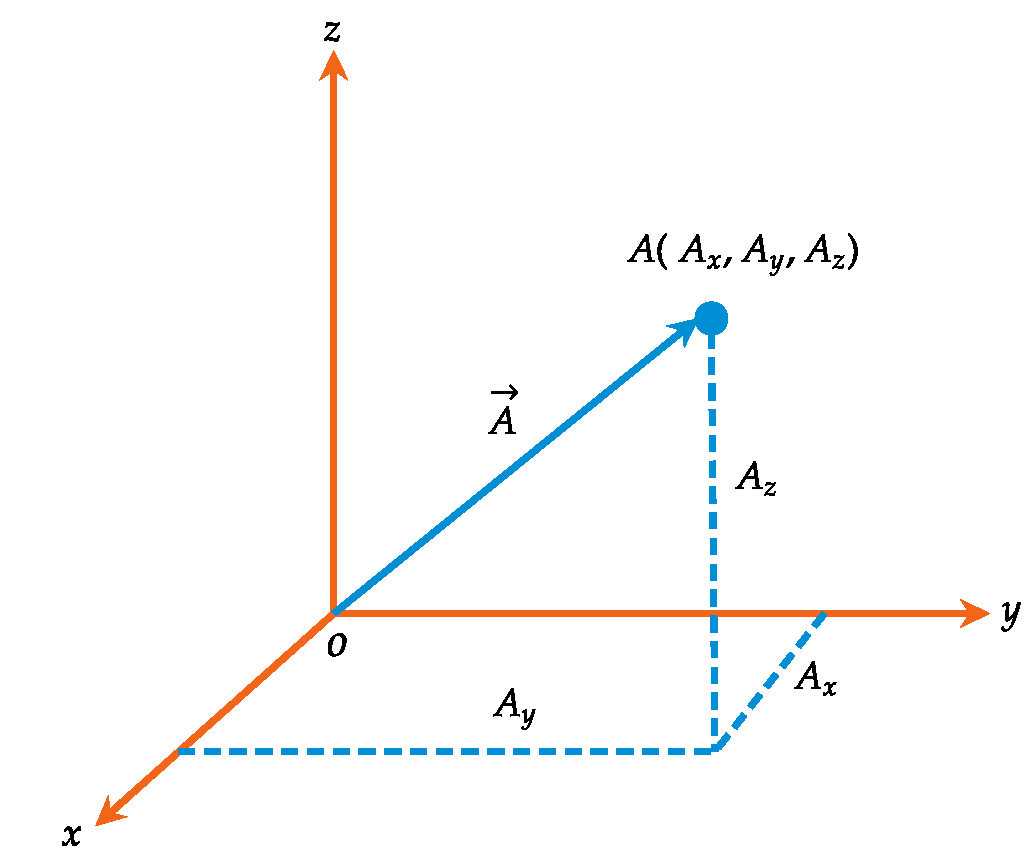
\includegraphics[width=0.4\textwidth]{vector2}
	\caption{Representation of position vector $\vec{A }$}
\end{figure}
 Any vector $\vec{\mathrm A}$ in the $3-\mathrm{\mathrm D}$ right handed rectangular cartesian coordinate system can be represented as,
 \begin{equation}
$$\vec{\mathrm A}=\mathrm A_{x} \hat{i}+\mathrm A_{y} \hat{j}+\mathrm A \hat{k}$$
 \end{equation} 
Where, $\hat{i}, \hat{j}$ and $\hat{k}$ are the unit vectors in direction of $x, y$ and $z$ axis respectively. $\mathrm A_{x}, \mathrm A_{y} $ and $ \mathrm A_{z}$ are the
cartesian components or projections of vector $\vec{A}$ along $x, y, z$ axis.
 \begin{exercise}
	 If $\mathrm A$ and $\mathrm B$ are (3,4,5) and $(6,8,9),$ find $\vec {\mathrm {A B}}$.
	\end{exercise}
\begin{answer}
$$\begin{aligned} \overrightarrow{\mathrm {A B}} &=\text { Position vector of } \mathrm B-\text { Position vector of } \mathrm A \\ &=(6 \hat{i}+8 \hat{j}+9 \hat{k})-(3 \hat{i}+4 \hat{j}+5 \hat{k}) \\ &=3 \hat{i}+4 \hat{j}+4 \hat{k} \end{aligned}$$
\end{answer}

\subsection{Unit vector:} 
\begin{definition}
	A vector quantity having unit magnitude is called unit vector.A unit vector along $\vec{A}$ is defined as,
	\\$\hat{\mathrm A}=\frac{\vec{\mathrm A}} {|\vec{\mathrm A}|}=\frac {\left(\mathrm A_{x} \hat{i}+\mathrm A_{y} \hat{j}+\mathrm A_{z} \hat{k}\right) } {\sqrt{\mathrm A_{x}^{2}+\mathrm A_{y}^{2}+\mathrm A_{z}^{2}}}$
\end{definition}
 \begin{exercise}
 	Find unit vector in the direction of vector $\vec{a}=2 \hat{i}+3 \hat{j}+\hat{k}$
 	 \end{exercise}
  \begin{answer}
  	
  	\begin{align*}
  		\text{Magnitude of }\vec{ a}&=\sqrt{2^{2}+3^{2}+1^{2}}\\
  		|\vec{a}|&=\sqrt{4+9+1}=\sqrt{14}\\
  		\text{Unit vector in direction of }\vec{a}&=\frac{\vec{a}}{| \vec{a}|}\\
  		\hat{a}&=\frac{1}{\sqrt{14}}[2 \hat{i}+3 \hat{j}+1 \hat{k}] \\
  		\hat{a}&=\frac{2}{\sqrt{14}} \hat{i}+\frac{3}{\sqrt{14}} \hat{i}+\frac{1}{\sqrt{14}} \hat{k}
  	\end{align*}
  	
  \end{answer}
  \subsection{Direction cosines}
In analytical geometry the direction cosines are the angles made by the vector with  the three coordinate axes.\\\\\textbf{Direction cosines of vector $\vec{\mathrm A}$} :
\\\newline If $\vec{\mathrm A}$ makes angles $\alpha, \beta, \gamma$ with $x, y$ and $z$ axes respectively, then direction cosines of $\vec{\mathrm A}$ are defined as,
\begin{minipage}{0.6\textwidth}
	\begin{flalign*}
	&l=\cos \alpha=\frac{\mathrm A_{x}}{\mathrm A}\quad ;\quad  m=\cos \beta=\frac{\mathrm A_{y}}{\mathrm A} \quad ;\quad  n=\cos \gamma=\frac{\mathrm A_{z}}{\mathrm A} \\  &l^{2}+m^{2}+n^{2}=1\\\\
	&\text{Then the unit vector along } \vec{\mathrm A}\text{ can be written as,}\\
	& \hat{\mathrm A}=l \hat{i}+m \hat{j}+n \hat{k}\\
	\end{flalign*}
\end{minipage}
\begin{minipage}{0.4\textwidth}
	\begin{figure}[H]
		\centering
		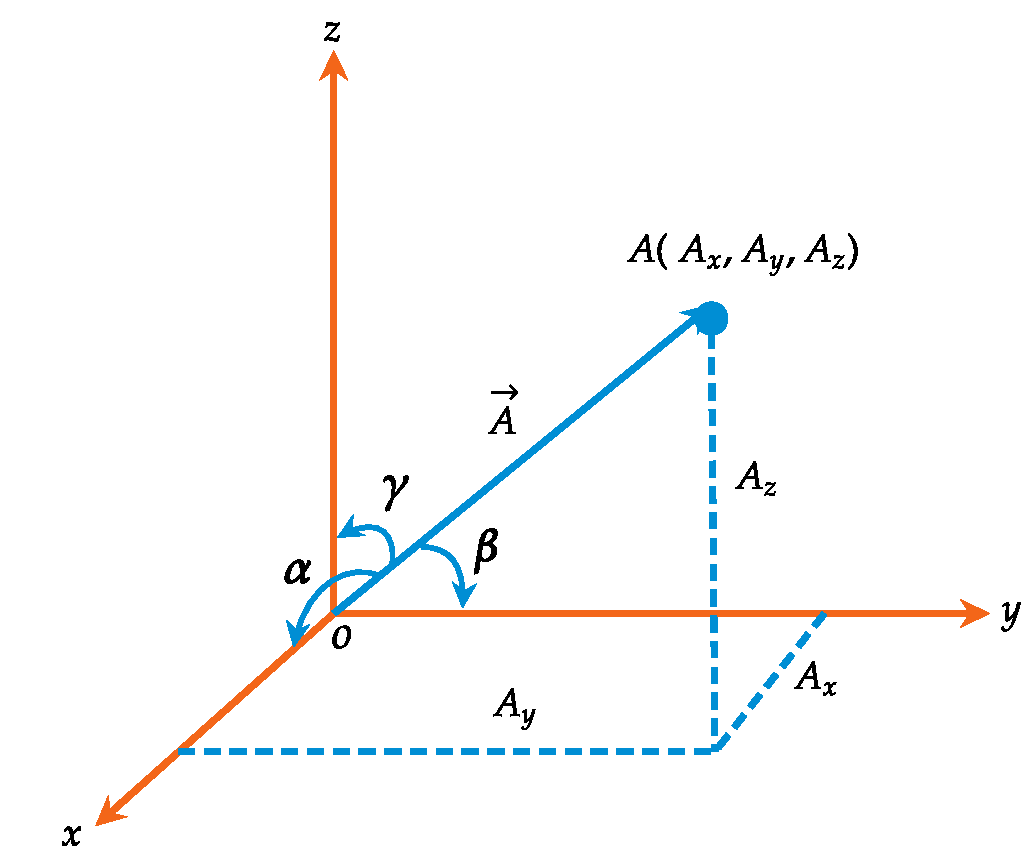
\includegraphics[width=6cm,height=6cm]{direction cosine}\caption{Direction cosine.}
	\end{figure}
\end{minipage}
\section{Types of vectors}
\begin{itemize}
	\item \textbf{{Equal vectors}}\hspace{0.74cm}\textbf{:}\quad Vectors having same magnitude and same direction.
	\item \textbf{Null Vectors }\hspace{0.82cm}\textbf{:} \quad Vectors having coincident initial and terminal point i.e its magnitude is zero and it has any arbitrary direction.
	\item \textbf{Reciprocal Vector }\textbf{:}\quad Vector having same direction as $\vec{\mathrm  A}$ but magnitude reciprocal to that of $\vec{\mathrm A},$ is known as the reciprocal vector of $\mathrm A$ Reciprocal vector of $\vec{\mathrm A}$ is $\vec{\mathrm A}-\frac{1}{\mathrm A} \hat{\mathrm A}$.
	\item \textbf{Negative Vector}\hspace{0.3cm} \textbf{:}\quad Vectors having same magnitude as $\vec{\mathrm a}$ but direction opposite to that of $\vec{\mathrm A},$ is known
	as the negative vector of $\vec{\mathrm a} .$ Negative vector as $\vec{\mathrm A}$ is $-\vec{\mathrm A}=-|\mathrm A| \hat{\mathrm A}$.
\end{itemize}
\section{Vector operations}\index{Vector operations}
\subsection{Vector addition}
\begin{itemize}
	\item 	\textbf{Triangular law of vector addition:}
	\begin{itemize}
		\item Place the tail of $\vec{\mathrm A}$ at the head of $\vec{\mathrm B} $.
		\item The resultant vector $\vec{\mathrm A}+\vec{\mathrm B}$ is formed by connecting the tail of the first vector to the head of the last vector. 
	\end{itemize}
\begin{figure}[H]
	\begin{minipage}{0.45\textwidth}
		\centering
		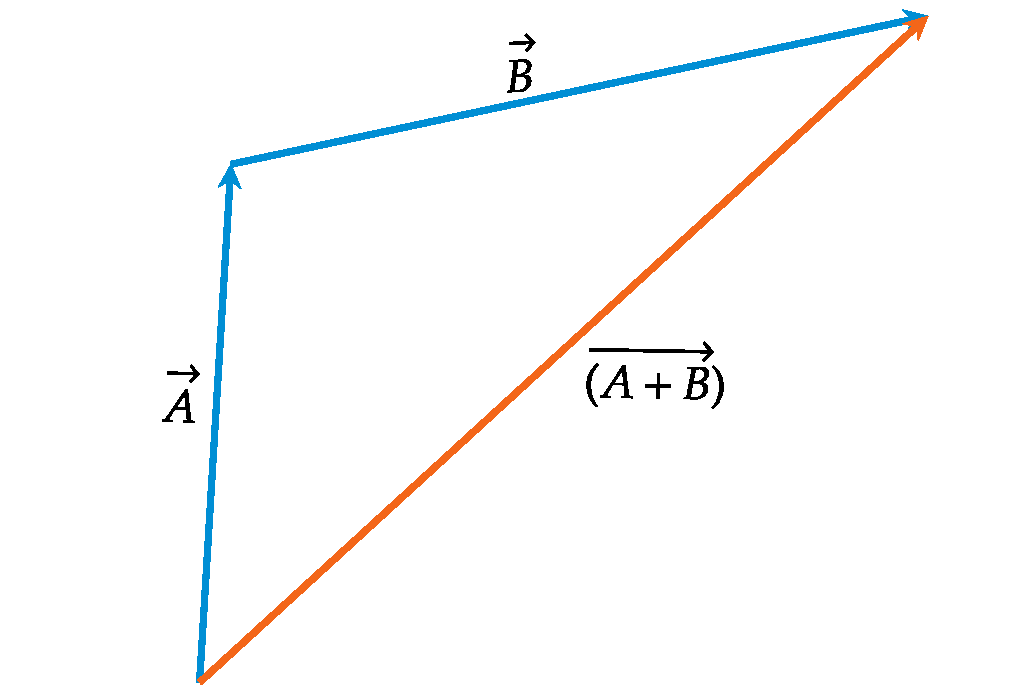
\includegraphics[width=0.70\textwidth]{Triangular}
		\caption{Triangular law of vector addition}
		\end{minipage}\hfil
	\begin{minipage}{0.45\textwidth}
	\centering
	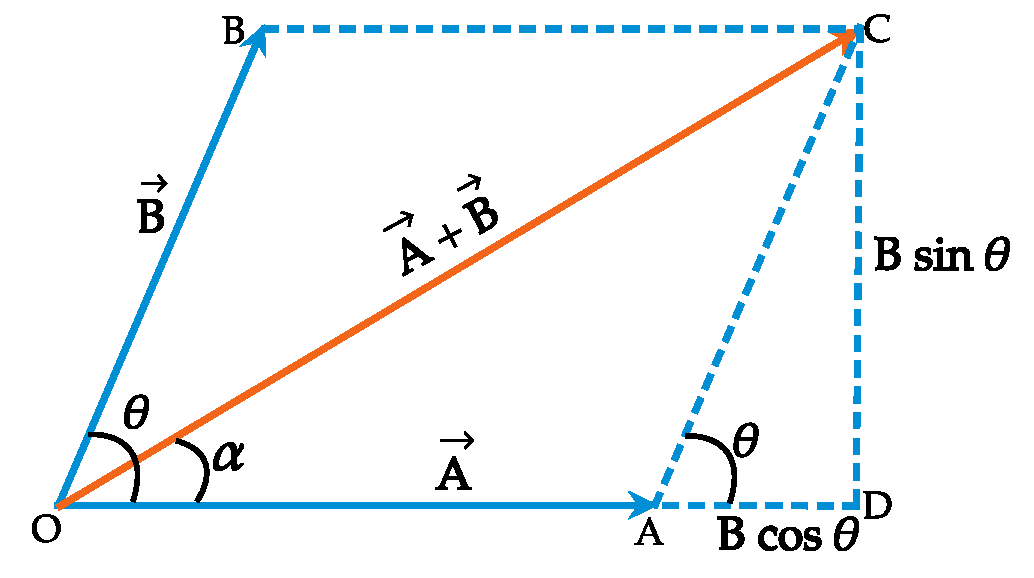
\includegraphics[width=0.75\textwidth]{parellelogram}
	\caption{Parellelogram law of vector addition}
\end{minipage}

\end{figure}

\item \textbf{Parellelogram law of vector addition:}
\\ \\When two vectors act at a point, their resultant is found by the law of parallelogram of vectors.(We got to use it often in Electricity and magnetism.)

The magnitude of Resultant vector ${\vec{A }+\vec{B}}$
From right angled $\triangle$ OCD.
\begin{align*}
O C^{2}&=O D^{2}+C D^{2}\\
&=(O A+AD)^{2}+C D^{2}\\
&=O A^{2}+A D^{2}+2AD\cdot OA +C D^{2}\\\\
\text{Here,}\hspace{1.3cm} O A&= A\ ; \ AD=B\cos\theta \ ; \ CD= B\sin\theta\\\\
\text{Then,}\hspace{1.1cm}  O C^{2}&=|\vec{A }+\vec{B}|^{2}\\&=A^{2}+(B\cos\theta)^{2}+(B\sin\theta)^{2}+2AB\cos\theta\\&=A^{2}+B^{2}+AB\cos\theta\\
|\vec{A }+\vec{B}|&=\sqrt{A^{2}+B^{2}+2AB\cos\theta}\\
\\
\text{The direction of }&\text{ Resultant vector}\ {\vec{A }+\vec{B}} \ \text{with the vector}  \ {\vec{A}}\\
\tan \alpha&=\frac{B \sin \theta}{A+B \cos \theta}\\
\alpha&=\tan ^{-1}\left(\frac{B \sin \theta}{A+B \cos \theta}\right)\\
\text{If the  two vectors}&\text{   are parellel i.e., $\theta=0$ \ Then,  }\ \\
|\vec{A }+\vec{B}|&=\sqrt{A^{2}+B^{2}+2AB}=\sqrt{(A+B)^{2}}=(A+B)\\
\text{If the  two vectors}&\text{   are anti-parellel i.e., $\theta=180$ \ Then,  }\ \\
|\vec{A }+\vec{B}|&=\sqrt{A^{2}+B^{2}-2AB}=\sqrt{(A-B)^{2}}=(A-B)\\
\end{align*}
\end{itemize}
\begin{note}
	\leavevmode
	\\\\
     	If $|\vec{A}|=|\vec{B}|=A$ Then resultant of these two vectors will be,
	\begin{enumerate}
		\item $\theta=0\qquad \rightarrow \sqrt{A^{2}+A^{2}+2A A\cos 0} \hspace{0.2cm}=\sqrt{A^{2}+A^{2}+2A^{2}}=2A $ 
		\item $\theta=60^{\circ} \quad\rightarrow \sqrt{A^{2}+A^{2}+2A A\cos 60}=\sqrt{A^{2}+A^{2}+A^{2}} =\sqrt{3}A $
		\item $\theta=90^{\circ}\quad\rightarrow \sqrt{A^{2}+A^{2}+2A A\cos 90}=\sqrt{A^{2}+A^{2}}=\sqrt{2} A $
			\item $\theta=180^{\circ} \hspace{0.3cm} \rightarrow \sqrt{A^{2}+A^{2}+2A A\cos 180}=\sqrt{A^{2}+A^{2}-2A^{2}} =0 $ 
	\end{enumerate}
\end{note}

\subsubsection{Properties of vector addition}
\begin{itemize}
	\item Commutation property:
	$\mathbf{A}+\mathbf{B}=\mathbf{B}+\mathbf{A}$.
	\item Associative property:$(\mathbf{A}+\mathbf{B})+\mathbf{C}=\mathbf{A}+(\mathbf{B}+\mathbf{C})$.
	\item Additive identity:$\mathbf{A}+\mathbf{0}=\mathbf{A} \quad$.
	\item Additive inverse:$\mathbf{A}+(-\mathbf{A})=\mathbf{0} \quad$ .
	
\end{itemize}
\subsection{Vector  multiplication}
\subsubsection{\large{1}.{Scaling of vector}(Multiplication by scalar)}
Scaling a vector means changing it's length by a scale factor.	Multiplication of a vector by a positive scalar $'c'$, multiplies the magnitude but leaves the
direction unchanged. If $'c'$ is negative, the direction is reversed.
\begin{figure}[H]
	\begin{center}
		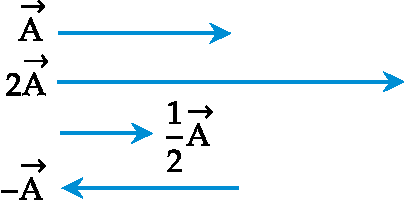
\includegraphics[width=0.30\textwidth]{scaling}
	\end{center}
\caption{Scaling of vector}
\end{figure}
\subsubsection{Properties of scalar multiplication}
\begin{itemize}
	\item  Distributive property:\quad$a(\vec{\mathrm A}+\vec{\mathrm B})=a \vec{\mathrm A}+a \vec{\mathrm B}$.
\end{itemize}
\subsubsection{\large{2}.Dot product or scalar product of two vectors}
The dot product of two vectors is defined as
\begin{equation}
$$\vec{A} \cdot \vec{B}=|A| | B| \cos \theta$$
\end{equation}
Where $\theta$ is the angle they form when placed tail to tail. $\vec{\mathrm{A}} \cdot \vec{\mathrm B}$ is itself a scalar.Geometrically $\vec{\mathrm A} \cdot \vec{\mathrm B}$ is the product of $\mathrm A$ times the projection of $\vec{\mathrm B}$ along $\vec{\mathrm A}$.
\\\newline In general,\ If \ $\vec{\mathrm A}=\mathrm A_{z} \hat{i}+\mathrm A_{y} \hat{j}+\mathrm A_{z} \hat{k}$ and $\vec{\mathrm B}=\mathrm B_{x} \hat{i}+\mathrm B_{y} \hat{j}+\mathrm B_{z} \hat{k},$\\\\ Then we can construct the scalar product of $\vec{\mathrm A}$ and $\vec{\mathrm B}$ as,
\begin{equation}
$$\vec{\mathrm A} \cdot \vec{ \mathrm B}=\mathrm A_{x} \mathrm B_{x}+\mathrm A_{y} \mathrm B_{y}+\mathrm A_{z} \mathrm B_{z}$$
\end{equation}  
\begin{example}\textbf{Workdone:}
	If a constant force $F$ acting on a particle displaces it from the point A to B then,\\
	\begin{minipage}{0.45\textwidth}
		\begin{align*}
		\text{Work done} &=\text{(component of F along A B ). Displacement}\\
		&=\mathrm{F} \cos \theta . A B \\
		&=\vec{F} \cdot \overrightarrow{A B}\\
		\text{Work done }&=\text{Force. Displacement}
		\end{align*}
	\end{minipage}
	\begin{minipage}{0.45\textwidth}
	\begin{figure}[H]
		\begin{center}
			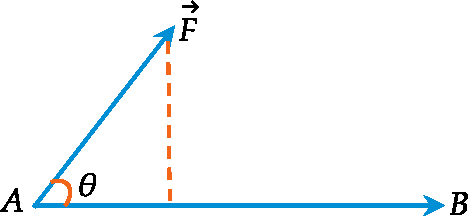
\includegraphics[width=0.65\textwidth]{workdone}
		\end{center}
		\caption{Workdone}
	\end{figure}
\end{minipage}
\end{example}
\subsubsection{Projection:}Projection of a vector A on B is the component of vector A in the direction of vector B.$$\text{Projection of}\quad \vec{\mathrm A} \text{\quad along}\quad \vec{\mathrm B} =\vec{\mathrm A}\cos\theta =\vec{\mathrm A} \cdot \hat{\mathrm B}$$.
\subsubsection{Properties of Dot product}
\begin{itemize}
	\item Commutative property:$\vec{\mathrm A} \cdot \vec{\mathrm B} =\vec{\mathrm B} \cdot \vec{\mathrm A}$.
	\item Asociative property:$ \vec{\mathrm A} \cdot(\vec{\mathrm B}+\vec{\mathrm C}) =\vec{\mathrm A} \cdot \vec{\mathrm B}+\vec{\mathrm A} \cdot \vec{\mathrm C}$.
	\item For two mutually perpendicular vectors $\vec{\mathrm A}$ and $\mathrm B, \mathrm A \cdot \vec{\mathrm B}=0$.
	\item If the two vectors are parallel, $\vec{\mathrm A} \cdot \vec{\mathrm B}=\mathrm {A B}$.(since, $\cos0=1$)
	\item $\hat{i} \cdot \hat{j}=\hat{j} \cdot \hat{k}=\hat{k} \cdot i=0\newline  \hat{i} \cdot \hat{i}=\hat{j}\cdot\hat{j} = \hat{k}\cdot \hat{k}=1$\\\\ 
\end{itemize}
\begin{exercise}
	For the two vectors  $ \vec{A}=6\hat{i}+4\hat{j}+3\hat{k}$ and $ \vec{B}=2\hat{i}-3\hat{j}-3\hat{k}$
	\newline  $$\begin{aligned}
	\vec{\mathrm A} \cdot \vec{ \mathrm B}&=\mathrm A_{x} \mathrm B_{x}+\mathrm A_{y} \mathrm B_{y}+\mathrm A_{z} \mathrm B_{z}\\
	&=12-12-9\\
	&=-9
	\end{aligned}$$
\end{exercise}
\subsubsection{{\large 3}.Vector  product or Cross product}
Cross product of two vectors $\vec{\mathrm A}$ and $\vec{\mathrm B}$  is defined as a vector that is perpendicular (orthogonal) to both $\vec{\mathrm A}$ and $\vec{\mathrm B}$, with  a magnitude equal to the area of the parallelogram that the vectors span(This suggest that area may be treated as a vector quantity). Since there are two opposite directions which are so perpendicular to $\vec{A} \ \text{and} \ \vec{B}$  This does not uniquely determine $\vec{A} \times \vec{B}$ . The direction of $\vec{A} \times \vec{B}$ is fixed by a convention, called the Right Hand Rule.\\\\
\textbf{Right Hand Rule :}\\
Stretch out the fingers of the right hand so that the thumb becomes perpendicular to both the index (fore
finger) and the middle finger. If the index points in the direction of $\vec{A}$ and the middle finger in the direction of
$\vec{B}$ then, $\vec{A} \times \vec{B}$ points in the direction of the thumb.\\\\
The vector product of $\vec{A} \ \text{and} \ \vec{B}$  is defined as, 
\begin{equation}
$$\vec{\mathrm A} \times \vec{\mathrm B}=|\vec{\mathrm A}||\vec{\mathrm B}| \sin \theta  \hat{n}$$
\end{equation}
Where $\hat{n}$ is unit vector normal to the plane containing $\vec{\mathrm A}$ and $\vec{\mathrm B}$.
\\Using decomposition of vector into their cartesian components,we can find $\vec{\mathrm A} \times \vec{\mathrm B}$ as,
\\ If $\vec{\mathrm A}=\mathrm A_{z} \hat{i}+\mathrm A_{y} \hat{j}+\mathrm A_{z} \hat{k}$ and $\vec{\mathrm B}=\mathrm B_{x} \hat{i}+\mathrm B_{y} \hat{j}+\mathrm B_{z} \hat{k},$ then $$\vec{\mathrm A} \times \vec{\mathrm B}=\left|\begin{array}{lll}\hat{i} & \hat{j} & \hat{k} \\ \mathrm A_{x} & \mathrm A_{y} & \mathrm A_{z} \\ \mathrm B_{x} & \mathrm B_{y} & B_{z}\end{array}\right|$$
\begin{example}
	Angular momentum
	\newline The angular momentum of a particle, about a reference point , is defined as the vector product of the potion relative to the reference point, and momentum of the particle
	 $$ L=r\times p$$
	 \begin{figure}[H]
	 	\begin{center}
	 		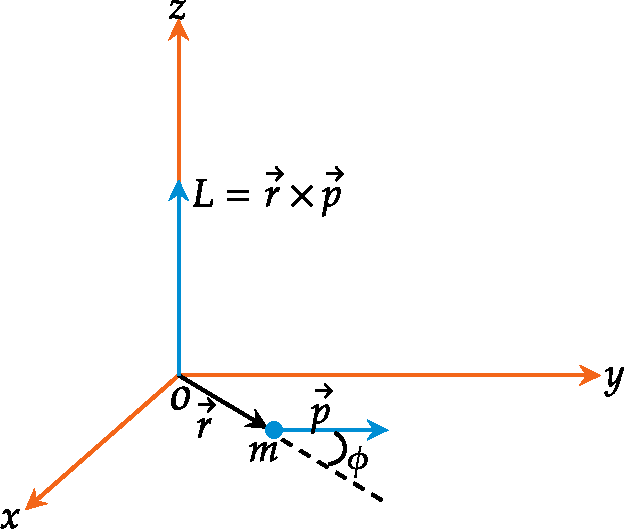
\includegraphics[width=0.30\textwidth]{angular momentum}
	 	\end{center}
 	\caption{Angular momentum}
	 \end{figure}
\end{example}
\subsubsection{Properties of Cross product} 
\begin{itemize}
	\item Distributive property\hspace{0.7cm}:\ $\vec{\mathrm A} \times(\vec{\mathrm B} + \vec{\mathrm C})=(\vec{\mathrm A} \times \vec{\mathrm B})+(\vec{\mathrm A} \times \vec{\mathrm C})$
	\item Commutative property\quad:\ $\vec{\mathrm A} \times \vec{\mathrm B}=-(\vec{\mathrm B} \times \vec{\mathrm A})$.
	\item For two collinear vectors (parallel or anti-parallel vectors) $\vec{\mathrm A} \times \vec{\mathrm B}=0$.
	\item $\hat{i} \times \hat{i}=\hat{j} \times \hat{j}=\hat{k} \times \hat{k}=0\\\\
	\; \ \hat{i} \times \hat{j}=\hat{k}
	\; \ \hat{j} \times \hat{k}=\hat{i}
	\; \ \hat{k} \times \hat{i}=\hat{j}$.
	
\end{itemize}
\begin{exercise}
	Find the area of a parallelogram whose adjacent sides are $\hat{i}-2 \hat{j}+3 \hat{k}$ and
	$2 \hat{i}+\hat{j}-4 \hat{k}$.
\end{exercise}
\begin{answer}
	\begin{align*}
\text{Vector area of parellelogram}&=\left|\begin{array}{rrr}\hat{i} & \hat{j} & \hat{k} \\ 1 & -2 & 3 \\ 2 & 1 & -4\end{array}\right|\\
&=(8-3) \hat{i}-(-4-6) \hat{j}+(1+4) \hat{k}=5 \hat{i}+10 \hat{j}+5 \hat{k}\\
\text{Area of parallelogram}&=\sqrt{(5)^{2}+(10)^{2}+(5)^{2}}=5 \sqrt{6}
\end{align*}
\end{answer}


\subsubsection{4.Triple product}
\begin{itemize}
	\item \textbf{Scalar Triple product}
	\\The scalar triple product of three vectors $\vec{\mathrm{A}}, \vec{\mathrm{B}}$, and $\vec{\mathrm{C}}$ is $(\vec{\mathrm{A}} \times\vec{\mathrm{B}}) \cdot \vec{\mathrm{C}} .$ It is a scalar product because, just like the dot product, it evaluates to a single number.  The absolute value of $|(\vec{\mathrm{A}} \times \vec{\mathrm{B}}) \cdot \vec{\mathrm{C}}|$ is the volume of the parallelepiped spanned by $\vec{\mathrm{A}}, \vec{\mathrm{B}},$ and $\vec{\mathrm{C}}$ (i.e., the parallelepiped whose adjacent sides are the vectors $\vec{\mathrm{A}}, \vec{\mathrm{B}},$ and $\vec{\mathrm{C}}$ ).\begin{figure}[H]
		\begin{center}
			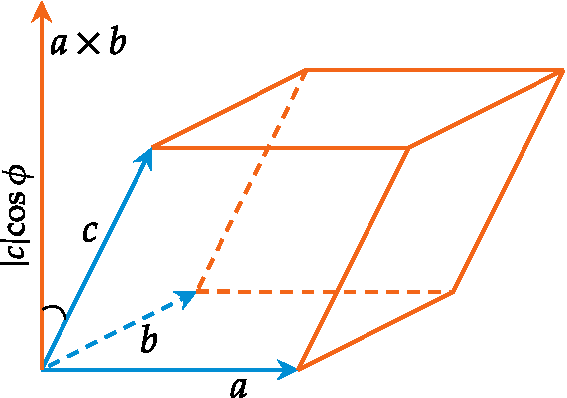
\includegraphics[width=0.25\textwidth]{parellelopiped}
		\end{center}
	\caption{Scalar triple product}
	\end{figure}
\begin{align*}
	\vec{\mathrm A} \cdot(\vec{\mathrm B} \times \vec{\mathrm C})&=\vec{\mathrm B} \cdot(\vec{\mathrm C} \times \vec{\mathrm A})=\vec{\mathrm C} \cdot(\vec{\mathrm A} \times \vec{\mathrm B})\\
	\text{In component form}\ \vec{\mathrm A} \cdot(\vec{\mathrm B} \times \vec{\mathrm C})&=\left|\begin{array}{lll}\mathrm A_{x} & \mathrm A_{y} & \mathrm A_{z} \\ \mathrm B_{x} & \mathrm B_{y} & \mathrm B_{z} \\ \mathrm C_{x} & \mathrm C_{y} & \mathrm C_{z}\end{array}\right|\\
\end{align*}

	\item \textbf{Vector Triple product}
	\\A vector triple product $\vec{\mathrm A} \times(\vec{\mathrm B} \times \vec{\mathrm C})$ of 3 vectors ,$\vec{\mathrm A}$ , $\vec{\mathrm B}$ and $\vec{\mathrm C}$ is simply a vector lying in the plane containing $\vec{\mathrm A}$ , $\vec{\mathrm B}$ and $\vec{\mathrm C}$.\\

	The vector triple product can be simplified by the so-called $\text{ B A C}-\text{ C A B}$ rule.The equation is linear in  A,B and C.
	$$
	\vec{\mathrm A} \times(\vec{\mathrm B} \times \vec{\mathrm C})=\vec{\mathrm B}(\vec{\mathrm A} \cdot \vec{\mathrm C})-\vec{\mathrm C}(\vec{\mathrm A} \cdot \vec{\mathrm B})
	$$
\end{itemize}
\begin{note}

Suppose we have two vectors $ \vec{a}$ and $ \vec {b}$ as shown in the figure.
\ref{vector}
We can write $\vec{b}$ as
$$\vec{b}=\vec{{b_{\parallel}}}+\vec{{b_{\perp}}} $$
Where ${b_{\parallel}}$ is the projection of $ \vec {b}$ along  $ \vec{a}$ and$ \vec{{b_{\perp}}}$ is the projection of  $ \vec {b}$ perpendicular to $ \vec{a}$\\
\begin{minipage}{0.65\textwidth}
	\begin{align*}
	\vec {b}=&(\vec{b}\cdot \hat{a})\cdot \hat{a}+\vec{{b_{\perp}}}\\
	\vec {b}=&\frac{(\vec{b}\cdot \vec{a})\cdot\vec{a}}{a^{2}}+\vec{{b_{\perp}}}\\
	\vec {b}=&\frac{(\vec{b}\cdot \vec{a})\cdot\vec{a}}{a^{2}}+{\vec{b}-\frac{(\vec{b}\cdot \vec{a})\cdot\vec{a}}{a^{2}}}\\
	\vec {b}=&\frac{(\vec{b}\cdot \vec{a})\cdot\vec{a}}{a^{2}}+\frac{\vec{b}(\vec{a}\cdot\vec{a})-{(\vec{b}\cdot\vec{a})\vec{a}}}{a^{2}}\\
	\vec {b}=&\frac{(\vec{b}\cdot \vec{a})\cdot\vec{a}}{a^{2}}+\frac{\vec{a}\times(\vec{b}\times\vec{a})}{a^{2}}\\
	\vec{b}=&\vec{{b_{\parallel}}}(\text{parellell component})+\vec{{b_{\perp}}}(\text{perpendicular component})
	\end{align*}
\end{minipage}
\begin{minipage}{0.35\textwidth}\hfill
\begin{figure}[H]
	\begin{center}
		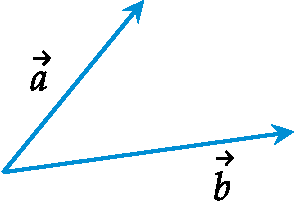
\includegraphics[width=0.8\textwidth]{vector1}
	\end{center}
\caption{vector}
\label{vector}
\end{figure}
\end{minipage}
\end{note}

\section{General curvilinear coordinate system}\index{General culvilinear coordinate system}
Not all Physical problems  are well adapted to a solution in cartesian coordinate system.We have to develop a general system that may be apt for any particular system of intersect.
The coordinates in general curvilinear coordinate system be described by three coordinates, $q_{1},q_{2} $ and $ q_{3}$\\then  a position vector $ \vec{ r}$ in the system can be represented as,
\begin{align*}
\vec{r}&=\vec{r}(q_{1},q_{2},q_{3})\\
\text{Then,}\quad
 dr&={\frac{\partial r}{\partial q_{1} }} dq_{1}+{\frac{\partial r}{\partial q_{2} }} dq_{2}+{\frac{\partial r}{\partial q_{3} }} dq_{3}
\end{align*}
Where,\ ${\frac{\partial r}{\partial q_{1} }}$,${\frac{\partial r}{\partial q_{2} }}$,${\frac{\partial r}{\partial q_{3} }}$ are the tangent vectors along $q_{1},q_{2}  $ and \ $q_{3}$.
\\\\The unit vectors along $q_{1},q_{2}  $ and \ $q_{3}$ are defined as,
$$ \hat e_{1}=\frac{{\frac{\partial r}{\partial q_{1} }}}{|{\frac{\partial r}{\partial q_{1} }}|}\quad ;\quad
 \hat e_{2}=\frac{{\frac{\partial r}{\partial q_{2} }}}{|{\frac{\partial r}{\partial q_{2} }}|}\quad ;\quad\hat e_{3}=\frac{{\frac{\partial r}{\partial q_{3} }}}{|{\frac{\partial r}{\partial q_{3} }}|}$$
\\
\textbf{Scaling factor:}\\\\
The factor ${|{\frac{\partial r}{\partial q_{1} }}|}$ is known as the scaling factor. It is denoted as $h_{1}$.\\\\
Similiarly, $h_{2}={|{\frac{\partial r}{\partial q_{2} }}|}$
and $h_{3}={|{\frac{\partial r}{\partial q_{3} }}|}$\\
\\Then the position vector can be written as,
\begin{equation}
$$ \vec dr=h_{1}\hat e_{1} dq_{1}+h_{2}\hat e_{2} q_{2}+h_{3}\hat e_{3}q_{3}$$
\end{equation}
\textbf{Cartesian coordinate system}
\begin{alignat*}{4}
&\text{Coordinates}&& \textbf{:} \ q_{1}=x\;\ q_{2}=y\;\ q_{3}=z\\
&\text{Scaling factors} && \textbf{:}\ h_{1}=1\; \ h_{2}=1\;\  h_{3}=1\\
&\text{Unit vectors}&&\textbf{:}\ \hat{e}_{1}=\hat{e}_{x}\;\ \hat{e}_{2}=\hat{e}_{y}\;\ \hat{e}_{3}=\hat{e}_{z}\\
&\text{Position vector}&&\textbf{:} \ \vec dr=\hat e_{x} dx+\hat e_{y} dy+\hat e_{z}dz
\end{alignat*}

\section{Differential Operations on Vectors}\index{Differential Operations on Vectors}
\begin{alignat*}{2}
&\text{Gradient }(\nabla)&&\textbf{:}\ \text{A derivative on a scalar that gives a vector.}
\\&\text{Curl} (\nabla \times)&&\textbf{:}\ \text{A derivative on a vector that gives another vector.}
\\&\text{Divergence }(\nabla \cdot)&&\textbf{:}\ \text{A derivative on a vector that gives scalar.}
\end{alignat*}
 
\subsection{Gradient}
 The gradient is the multidimensional rate of change of a particular function.
Gradient of a continuously differentiable scalar function $\phi(q_{1}, q_{2}, q_{3})$ is mathematically defined as:
$$ \nabla \phi=\frac{1}{h_{1}}\frac{\partial \phi}{\partial q_{1}} \hat e_{1}+\frac{1}{h_{2}}\frac{\partial \phi}{\partial q_{2}} d \hat e_{2}+\frac{1}{h_{3}}\frac{\partial \phi}{\partial q_{3}} \hat e_{3}
$$
\subsubsection{Physical interpretation}
	Gradient tells you how much something changes as you move from one point to another (such as the pressure in a stream). If a surface $\phi(x, y, z)=c$ passes through a point $P$. The value of the function at each point on the surface is the same as at $P$. Then such a surface is called a level surface through $P$. At each point of the level surafce, the value of scalar function $f$ will be same. Equipotential surface on which value of electrostatic potential is same at all points.


	\begin{figure}[H]
		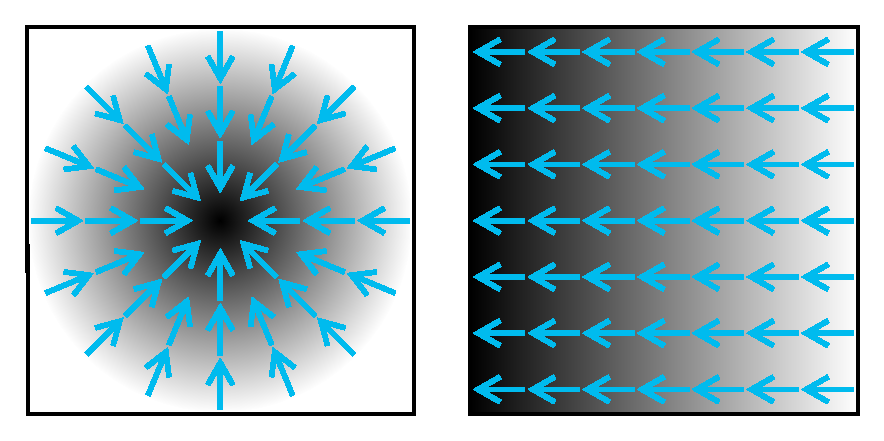
\includegraphics[width=.85\textwidth]{Gradient2}
		\caption{The gradient, represented by the blue arrows, denote the direction of greatest change of a scalar function. The values of the function are represented in greyscale and increase in value from white (low) to dark (high).}
	\end{figure}




\subsubsection{Product rule}$ \bullet$ $\vec{\nabla}(\phi \psi)=\phi \vec{\nabla} \psi+\psi \vec{\nabla} \phi$
\\$ \bullet$ $\vec{\nabla}(\overrightarrow{\mathrm{A}} \cdot \overrightarrow{\mathrm{B}})=\overrightarrow{\mathrm{A}} \times(\vec{\nabla} \times \overrightarrow{\mathrm{B}})+\overrightarrow{\mathrm{B}} \times(\vec{\nabla} \times \overrightarrow{\mathrm{A}})+(\overrightarrow{\mathrm{A}} \cdot \vec{\nabla}) \overrightarrow{\mathrm{B}}+(\overrightarrow{\mathrm{B}} \cdot \vec{\nabla}) \overrightarrow{\mathrm{A}}$
\\
\\\textbf{Normal and Directional derivative}
 \\\\\textbf{ Normal:}\newline If $\phi(x, y, z)=c$,  represents a family of surfaces for different values of the constant
 c. On differentiating $\phi,$ 

\begin{align*}
	 \text{We get,} \hspace{0.8cm}  d \phi&=0
	\\\text{But,} \hspace{0.8cm} d \phi&=\nabla \phi \cdot d \vec{r} \quad \\
	\text{So,} \hspace{0.05cm} \quad \nabla \phi \cdot d r&=0
	\end{align*}
The scalar product of two vectors $\nabla \phi$ and $d \vec{r}$ being zero, $\nabla \phi$ and $d \vec{r}$ are perpendicular to each other. Then, $d \vec{r}$ is in the direction of tangent to the given surface.

	\begin{itemize}
	\item  Normal vector to the level surface\hspace{1.2cm}: $\vec{\nabla} \phi$ 
	\item   Unit normal vector to the level surface\quad: $\hat{n}=\frac{\vec{\nabla} \phi}{|\vec{\nabla} \phi|}$
\end{itemize}
	
\begin{exercise}
	 Find the unit normal to the surface:$x^{2}+y^{2}=z$ at a point (1,2,5) \end{exercise}
	 \begin{answer}
	 		\begin{align*}
	 		\text{Let}\ \phi&=x^{2}+y^{2}-z\\
	 		\nabla \phi&=\left(\hat{i} \frac{\partial}{\partial x}+\hat{j} \frac{\partial}{\partial y}+\hat{k} \frac{\partial}{\partial z}\right)\left(x^{2}+y^{2}-z\right)=2 x \hat{i}+2 y \hat{j}-\hat{k}\\
	 		(\nabla \phi)_{1,2,5}&=2 \hat{i}+4 \hat{j}-\hat{k}\\
	 		\text { Unit normal vector }&=\frac{\Delta \phi}{|\Delta \phi|}\\&=\frac{2 \hat{i}+4 \hat{j}-\hat{k}}{\sqrt{4+16+1}}\\&=\frac{2}{\sqrt{21}} \hat{i}+\frac{4}{\sqrt{21}} \hat{j}-\frac{\hat{k}}{\sqrt{21}}
	 	\end{align*}
	 \end{answer}

	
 \subsubsection{Directional derivative} Directional derivative of $\phi$ in the direction of $\vec{A}$ is defined as rate of change of
$\phi$ with distance along the direction of $\vec{A}$. It is mathematically defined as the component of $\vec{\nabla} \phi$ in the direction of vector $\vec{A}$ i.e.
\begin{equation*}
 \vec{\nabla} \phi\cdot{{\hat A}}=\vec{\nabla} \phi.\frac{\vec A}{|\vec{A}|}
\end{equation*}
\begin{exercise}
	Find the directional derivative of $\phi(x, y, z)=x^{2} y z+4 x z^{2}$ at (1,-2,1) in the direction of $2 \hat{i}-\hat{j}-2 \hat{k}$.\end{exercise}
\begin{answer}
		\begin{align*}
		\phi(x, y, z)&=x^{2} y z+4 x z^{2}\\
		\nabla \phi&=\left(\hat{i} \frac{\partial}{\partial x}+\hat{j} \frac{\partial}{\partial y}+\hat{k} \frac{\partial}{\partial z}\right)\left(x^{2} y z+4 x z^{2}\right)\\
		&=\left(2 x y z+4 z^{2}\right) \hat{i}+\left(x^{2} z\right) \hat{j}+\left(x^{2} y+8 x z\right) \hat{k} \\
		\nabla \phi \text { at }(1,-2,1) &=\left\{2(1)(-2)(1)+4(1)^{2}\right\} \hat{i}+(1 \times 1) \hat{j}+\{1(-2)+8(1)(1)\} \hat{k} \\
		&=(-4+4) \hat{i}+\hat{j}+(-2+8) \hat{k}=\hat{j}+6 \hat{k} \\
		\hat{a} &=\text { unit vector }=\frac{2 \hat{i}-\hat{j}-2 \hat{k}}{\sqrt{4+1+4}}=\frac{1}{3}(2 \hat{i}-\hat{j}-2 \hat{k})
		\intertext{So, the  directional derivative at (1,-2,1)}&=\nabla \phi \cdot \hat{a}\\
		&=(\hat{j}+6 \hat{k}) \cdot \frac{1}{3}(2 \hat{i}-\hat{j}-2 \hat{k})\\&=\frac{1}{3}(-1-12)=\frac{-13}{3}
	\end{align*}
\end{answer} 
\subsubsection{Tangent planes}
\vspace{-0.8cm}
\begin{minipage}{0.6\textwidth}
	Consider $\phi(x, y, z)=c$ be the equation of a level surface, and $\vec{r}=x_{0} i+y_{0}\hat{j}+z_{0} \hat{k}$ be the position vector of
any point $\mathrm{P}(x, y, z)$ on this surface. \\\\Since, $ \vec{\nabla} \phi$ is a vector normal to the surface, it is perpendicular to the tangent plane at
P. 
\end{minipage}
\begin{minipage}{0.4\textwidth}
	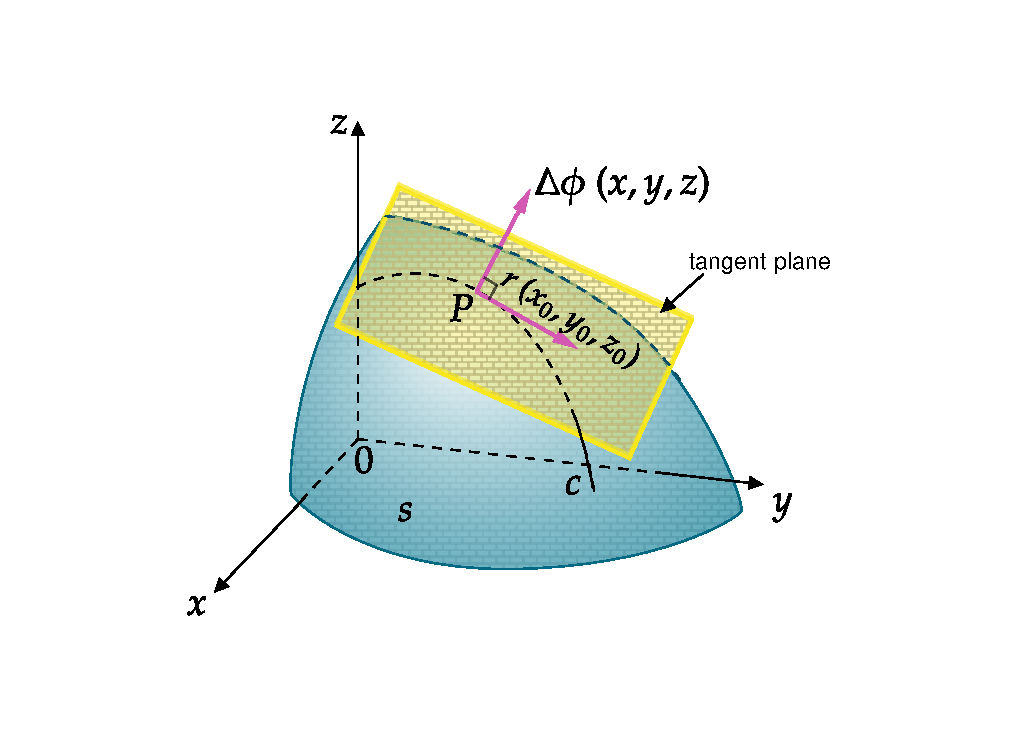
\includegraphics[width=8cm]{tangent plane}
\end{minipage}


 Let, $\vec{R}=x\hat{i}+y \hat{j}+z\hat{k}$ be the position vector of any point on the tangent plane at $P$ to the surface.\\\\  Then,
$\vec{R}-\vec{r}=(x-x_{0}) \hat{i}+(y-y_{0}) \hat{i}+(z-z_{0}) \hat{k}$ lies in the tangent plane at $P$ and it will be perpendicular to $\vec{\nabla} \phi$
\\Then the tangent plane at the point P :\begin{align*}
(\vec{R}-\vec{r}) \cdot \vec{\nabla} \phi&=0\\
(x-x_{0}) \frac{\partial \phi}{\partial x}+(y-y_{0}) \frac{\partial \phi}{\partial y}+(z-z_{0}) \frac{\partial \phi}{\partial z}&=0
\end{align*}

 


%...........................................................................................
\subsection{Divergence ($\nabla \cdot$)}
The divergence of a vector field measures how much the flow is expanding at a given point. It does not indicate in which direction the expansion is occuring. Hence the divergence is a scalar. Divergence of a continuous differentiable vector point function $A$ specified in a vector field is given
by,
$$
{\nabla} \cdot \vec{f}=\frac{1}{h_{1} h_{2} h_{3}}\left[\frac{\partial}{\partial q_{1}}\left(h_{2} h_{3} f_{1}\right)+\frac{\partial}{\partial q_{2}}\left(h_{3} h_{1} f_{2}\right)+\frac{\partial}{\partial q_{3}}\left(h_{1} h_{2} f_{3}\right)\right]
$$
In Cartesian coordinate system,

$$ \nabla.f=\frac{\partial f_{1}}{\partial x}+\frac{\partial f_{2}}{\partial y}+\frac{\partial f_{3}}{\partial z}$$
You can't
have the divergence of a scalar: that’s meaningless.


\subsubsection{Physical interpretation}
$\vec{\nabla} \cdot \vec{A}$ is a measure of how much the vector $\vec{A}$ spreads out (diverges) from a point in space.
\begin{figure}[H]
	\begin{center}
		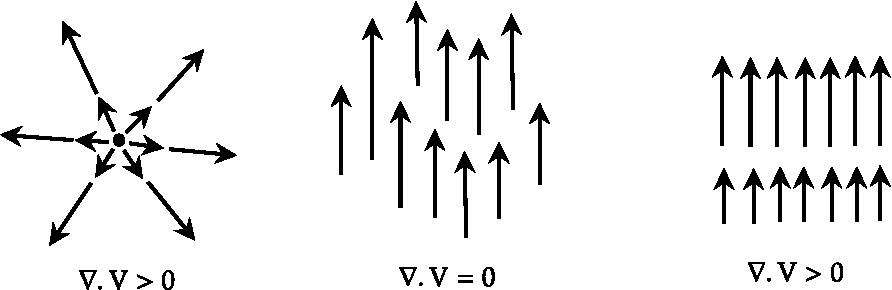
\includegraphics[width=9cm,height=3cm]{divergence-crop}
	\end{center}
\caption{Physical intepretation of divergence.}
\end{figure}

\begin{note}
	$\bullet$ If $\vec{\nabla} \cdot \vec{A}=0,$ then $\vec{A}$ is known as solenoidal vector field.
	\\$\bullet$ If $\vec{\nabla} \cdot \vec{A}=$ negative, then $\vec{A}$ is known as sink field i.e. vector lines are going inward.
	\\$\bullet$ If $\vec{\nabla} \cdot \vec{A}=$ positive, then $\vec{A}$ is known as source field i.e. vector lines are the going outward.
\end{note}
\textbf{Product rules}\\\\$\bullet$ $\vec{\nabla} \cdot(f \overrightarrow{\mathrm{A}})=f(\vec{\nabla} \cdot \overrightarrow{\mathrm{A}})+\overrightarrow{\mathrm{A}} \cdot(\vec{\nabla} f)$
$\\\bullet \vec{\nabla} \cdot(\vec{A} \times \vec{B})=\vec{B} \cdot(\vec{\nabla} \times \vec{A})-\vec{A} \cdot(\vec{\nabla} \times \vec{B})$
\begin{exercise}
	 
	Calculate $\nabla \cdot \vec{ r}$\end{exercise}
	 \begin{answer}
	 
	 \begin{align*}
	 	\vec{ r}&=x\hat{i}+y\hat{j}+z\hat{k}\\
	 	\nabla \cdot \vec{ r} &=\left(\hat{i} \frac{\partial}{\partial x}+\hat{j} \frac{\partial}{\partial y}+\hat{k} \frac{\partial}{\partial z}\right) \cdot (x\hat{i}+y\hat{j}+z\hat{k})\\
	 	&=\frac{\partial x}{\partial x}+\frac{\partial y}{\partial y}+\frac{\partial z}{\partial z}\\
	 	&=1+1+1\\
	 	&=3
	 \end{align*}
	 
	 
	 \end{answer}
	 
	 

\subsection{Curl}
The curl is the vector valued derivative of a vector function. Its operation can be geometrically interpreted as the rotation of a field about a point in space.\\From the definition of $\vec{\nabla}$ we construct the curl of a vector $\vec{f}=f_1\hat{e}_{1}+f_2\hat{e}_{2}+f_3\hat{e}_{3}$ as
$$
\nabla \times \vec{f
}=\frac{1}{h_{1} h_{2} h_{3}}\left|\begin{array}{lll}
	h_{1} \hat{e}_{1} & h_{2} \hat{e}_{2} & h_{3} \hat{e}_{3} \\
	\partial / \partial q_{1} & \partial / \partial q_{2} & \partial / \partial q_{3} \\
	h_{1} f_{1} & h_{2} f_{2} & h_{3} f_{3}
\end{array}\right|
$$
In cartesian coordinate system,
$$
\nabla \times \vec{f
}=\left|\begin{array}{lll}
\hat{{i}} & \hat{{j}} & \hat{{k}} \\
\partial / \partial x & \partial / \partial y & \partial / \partial z \\
f_{1} & f_{2} & f _{3}
\end{array}\right|
$$

%...........................................................................................
\subsubsection{Physical interpretation}
\begin{figure}[H]
	\begin{center}
		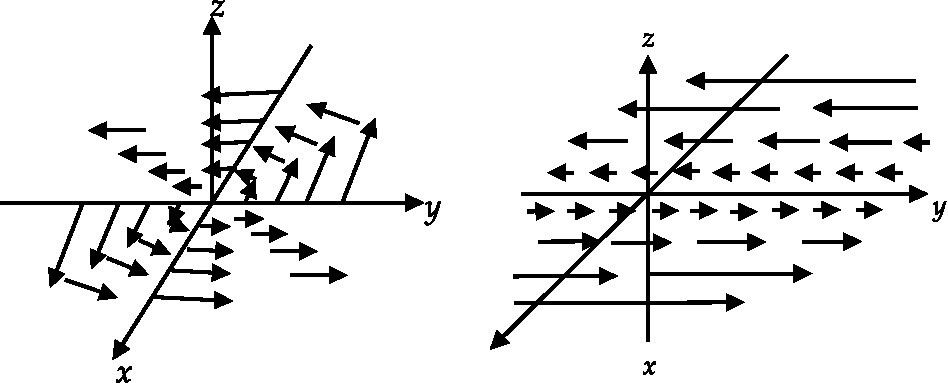
\includegraphics[width=9cm,height=4cm]{coordinate2}
	\end{center}
	\caption{Physical interpretation of Curl}
\end{figure}
The curl of a vector field measures the tendency for the vector field to swirl around. Imagine that the vector field represents the velocity vectors of water in a lake. If the vector field swirls around, then when we stick a paddle wheel into the water, it will tend to spin. The amount of the spin will depend on how we orient the paddle. Thus, we should expect the curl to be vector valued.\\
\\$\bullet \ $ If $\vec{\nabla} \times \vec{V}=0,$ then $\vec{V}$ is known as an irrotational vector and we can write $\vec{V}=\vec{\nabla} \phi$
\\$\bullet \ $ If $\vec{\nabla} \times \vec{V} \neq 0,$ then $\vec{V}$ is known as rotational vector.
\\\\\textbf{Product rules}\\
\\$\bullet \ \vec{\nabla} \times(f \overrightarrow{\mathrm{A}})=f(\vec{\nabla} \times \overrightarrow{\mathrm{A}})-\overrightarrow{\mathrm{A}} \times(\vec{\nabla} f)$
$\\\bullet \ \vec{\nabla} \times(\overrightarrow{\mathrm{A}} \times \overrightarrow{\mathrm{B}})=(\overrightarrow{\mathrm{B}} \cdot \vec{\nabla} ) \overrightarrow{\mathrm{A}}-(\overrightarrow{\mathrm{A}} \cdot \vec{\nabla}) \overrightarrow{\mathrm{B}}+\overrightarrow{\mathrm{A}}(\vec{\nabla} \cdot \overrightarrow{\mathrm{B}})-\overrightarrow{\mathrm{B}}(\vec{\nabla} \cdot \overrightarrow{\mathrm{A}})$

\begin{exercise}
	 Prove that $\left(y^{2}-z^{2}+3 y z-2 x\right) \hat{i}+(3 x z+2 x y) \hat{j}+(3 x y-2 x z+2 z) \hat{k}$ is  irrotational.\end{exercise}
	\begin{answer}
		For irrotational, we have to prove Curl $\bar{F}=0$.
		\begin{align*}
		\operatorname{Curl} \vec{F}&=\left|  \begin{array}{lll}
		\hat{i} & \hat{j} & \hat{k} \\
		\frac{\partial}{\partial x} & \frac{\partial}{\partial y} & \frac{\partial}{\partial z} \\
		y^{2}-z^{2}+3 y z-2 x & 3 x z+2 x y & 3 x y-2 x z+2 z
		\end{array}\right| \\
			&=(3 x-3 x) \hat{i}-(-2 z+3 y-3 y+2 z) \hat{j}+ 
		(3 z+2 y-2 y-3 z) \hat{k}\\&=0 \hat{i}+0 \hat{j}+0 \hat{k}=0
			\intertext{Thus, $\vec{F}$ is irrotational.}
		\end{align*}
		\end{answer}
	\begin{note}
		\begin{enumerate}
			\item The divergence of a curl of a vector field vanishes.
			\\$ \nabla \cdot(\nabla \times u)=0$\\If $ \nabla \cdot v=0 \Longrightarrow v= \nabla \times u$
			\item The curl of gradient of a scalar field vanishes.
			\\$ \nabla \times(\nabla \phi)=0$\\If $ \nabla \times \psi=0 \Longrightarrow \psi= \nabla  u$
		\end{enumerate}
	\end{note} 


\subsection{Laplacian}

The divergence of the gradient of a scalar function is called the Laplacian. In general culvilinear coordinate system laplacian can be written as,
\begin{align*}
\nabla^{2}=\frac{1}{h_{1} h_{2} h_{3}}\left[\frac{\partial}{\partial u_{1}}\left(\frac{h_{2} h_{3}}{h_{1}} \frac{\partial}{\partial u_{1}}\right)+\right. 
\left. \frac{\partial}{\partial u_{2}}\left(\frac{h_{1} h_{3}}{h_{2}} \frac{\partial}{\partial u_{2}}\right)+\frac{\partial}{\partial_{u_{3}}}\left(\frac{h_{1} h_{2}}{h_{3}} \frac{\partial}{\partial_{u_{3}}}\right)\right]
\end{align*}

In cartesian coordinate sytem,
$$ \nabla^{2}=\frac{\partial^{2}}{\partial x^{2}}+\frac{\partial^{2}}{\partial y^{2}}+\frac{\partial^{2}}{\partial z^{2}}$$
\begin{table}[h]
	\overfullrule=0pt
	\begin{tabular}{|p{1.8cm}|p{6cm}|p{8.5cm}|}
		\hline
		
		&\textbf{Cylindrical polar}($ \rho,\phi,z$) & \textbf{Spherical polar}(r,$\theta$,$\phi$)  \\\hline
		Scale factor&  ${\begin{array}{l}
				h_{1}=1  \\
				h_{2}=r \\
				h_{3}=1
		\end{array}}$ &${\begin{array}{l}
				h_{1}=1  \\
				h_{2}=r \\
				h_{3}=r \sin \theta
		\end{array}}$   \\\hline
		Gradient& $$
		\frac{\partial {f}}{\partial \boldsymbol{\rho}} \hat{\rho}+\frac{1}{\rho}\frac{\partial {f}}{\partial {\phi}} \hat{\phi}+\frac{\partial {f}}{\partial {z}} \hat{{z}}
		$$\vspace{1cm}&$$
		\hat{{r}} \frac{\partial f}{\partial r}+\hat{\boldsymbol{\theta}} \frac{1}{r} \frac{\partial f}{\partial \theta}+\hat{{\phi}} \frac{1}{r \sin \theta} \frac{\partial f}{\partial \phi}
		$$\\\hline
		Divergence\vspace{1cm}& $$
		\frac{1}{\rho} \frac{\partial }{\partial \rho}\left(\rho F_{\rho}\right)+\frac{1}{\rho} \frac{\partial }{\partial \phi}\left(F_{\phi}\right)+\frac{\partial }{\partial z}\left(F_{z}\right)
		$$ & $$
		\frac{1}{\mathrm{r}^{2}} \frac{\partial}{\partial \mathrm{r}}\left(r^{2} F_{\mathrm{r}}\right)+\frac{1}{\mathrm{rsin} \theta} \frac{\partial}{\partial \theta}\left(F_{\theta} \sin \theta\right)+\frac{1}{r \sin \theta} \frac{\partial \mathrm{F}_{\phi}}{\partial \phi}
		$$ \\\hline
		Curl\vspace{1cm}&$$
		\frac{1}{\rho } \left|\begin{array}{ccc}
			\hat{\rho} & \hat{\phi} & \hat{{z}} \\
			\frac{\partial}{\partial \boldsymbol{\rho}} & \frac{\partial}{\partial \phi} & \frac{\partial}{\partial \mathbf{z}} \\
			{F}_{\rho} & {F}_{\phi} & {F}_{{z}}
		\end{array}\right|
		$$ &$$
		\frac{1}{r^{2} \sin \theta}\left|\begin{array}{ccc}
			\hat{e}_{r} & r \hat{e}_{\theta} & r \sin \theta \hat{e}_{\phi} \\
			\partial / \partial r & \partial / \partial \theta & \partial / \partial \phi \\
			F_{r} & r F_{\theta} & r \sin \theta F_{\phi}
		\end{array}\right|
		$$ \\\hline
	Laplacian	& $$\frac{\partial^{2} f}{\partial r^{2}}+\frac{1}{r} \frac{\partial f}{\partial r}+\frac{1}{r^{2}} \frac{\partial^{2} f}{\partial \theta^{2}}+\frac{\partial^{2} f}{\partial z^{2}}$$ &$$
	\frac{1}{\mathrm{r}^{2}} \frac{\partial}{\partial \mathrm{r}}\left(r^{2} \frac{\partial f}{\partial r}\right)+\frac{1}{\mathrm{r^{2}sin} \theta} \frac{\partial}{\partial \theta}\left( \sin \theta \frac{\partial f}{\partial \theta}\right)+\frac{1}{r^{2} \sin^{2} \theta} \frac{\partial^{2} f}{\partial \phi^{2}}
	$$ 
	\\\hline

	\end{tabular}
\label{differential operators}
\caption{Differential operators in general culvilinear coordinate system}
\end{table}
\vspace{1cm}
	



\subsection{Important identities}
\begin{enumerate}
	 
	\item $\nabla \cdot \nabla \vec{A}=\nabla^{2} A=\frac{\partial^{2} \vec{A}}{\partial x^{2}}+\frac{\partial^{2} \vec{A}}{\partial y^{2}}+\frac{\partial^{2} \vec{A}}{\partial z^{2}}$( The Laplace operator.)
\item $\nabla \times \nabla \vec{A}=0$
\item $\nabla \cdot \nabla \times \vec{A}=0$
	\item $\nabla \times(\nabla \times \vec{A})=\nabla(\nabla \cdot \vec{A}) \times \nabla^{2} \vec{A}$
	\item $\nabla(\nabla \cdot \vec{A})=\nabla \times(\nabla \times \vec{A})+\nabla^{2} \vec{A}$
	\item $\nabla(\vec{A}+\vec{B})=\nabla \cdot \vec{A}+\nabla \cdot \vec{B}$
\item $\nabla \times(\vec{A}+\vec{B})=\nabla \times \vec{A}+\nabla \times \vec{B}$
\item $\nabla \cdot(\vec{A} \times \vec{B})=\vec{B} \cdot(\nabla \times \vec{A})-\vec{A} \cdot(\nabla \times \vec{B})$
\item $\nabla \times(\vec{A} \times \vec{B})=(B \cdot \nabla) A-B(\nabla \cdot A)-(A \nabla)$
$\quad B+A(\nabla B)$
\end{enumerate}
\section{Integral Calculus}
\subsection{Line integration of vectors}
\begin{figure}[H]
	\begin{center}
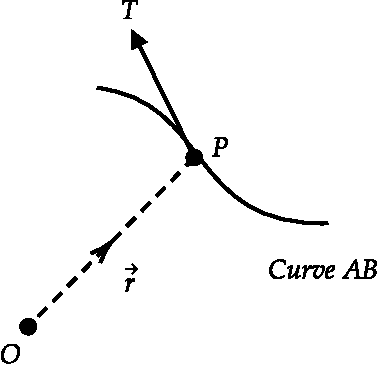
\includegraphics[width=3cm,height=3cm]{cs-01-crop}
		
	\end{center}
\caption{Line integration}
\label{line integration}	
\end{figure}
The integration of a vector function $\vec F$ along a curve is known as line integration of vectors.Infact the line integral along the curve is the integral of $\vec F$ along the tangent to the curve. 
 Consider a pont P in the curve in figure \ref{line integration} such that the position vector of P is given by $\vec r$.\\The component of $\vec F$ along the tangent at P = $\left(\vec{F} \cdot \frac{d \vec{r}}{d s}\right)$ \newline Then the Line integral of $\vec{F}$ from $A$ to $B$ along the curve $C$ will be, 
 $$\text{ Line integral}=\int_{c}\left(\vec{F} \cdot \frac{d \vec{r}}{d s}\right) d s=\int_{c} \vec{F} \cdot d \vec{r}$$


\begin{note}
	\begin{itemize}
		\item If $\vec{F}$ represents the variable force acting on a particle along arc $\mathrm{AB}$, then the total work done
		$W_{A B}=\int_{A}^{B} \vec{F} \cdot d \vec{r}$ 
		\item  If $\vec{V}$ represents the velocity of a liquid then $\oint_{c} \vec{V} \cdot d \vec{r}$ is called the circulation of $\vec{V}$ round closed curve
		$C$
		\item When the path of integration is a closed curve then notation of integration is $\oint$ in place of $\int$.
	\end{itemize}
\end{note}
\begin{example}
\textbf{Workdone}
\\  Work done by a conservative field $\vec{A}$ in moving a particle from point $P$ to $Q$ will be
$$
\int_{P}^{Q} \vec{F} \cdot \overrightarrow{d r}=\int_{P}^{Q} \vec{\nabla} \phi \cdot \overrightarrow{d r}=\int_{P}^{Q} d \phi=\phi_{Q}-\phi_{P}=\text { independent of path. }
$$
\\ Ordinarily, the value of a line integral depends critically on the particular path taken from
$a$ to $b$, but there is an important special class of vector functions for which the line
integral is independent of the path, and is determined entirely by the end points $($ A force
that has this property is called conservative).\\$\vec{A}$ in moving a particle around a closed path $C$ is $\oint_{c} \vec{F} \cdot \overrightarrow{d r}=0$
\end{example}
\begin{exercise}
	 If a force $\vec{F}=2 x^{2} y \hat{i}+3 x y \hat{j}$ displaces a particle in the xy-plane from (0,0) to
	(1,4) along a curve $y=4 x^{2} .$ Find the work done.\end{exercise}
	\begin{answer}
		\begin{align*}
		\text{Work done}&=\int_{c} \vec{F} \cdot \overrightarrow{d r} \\
		&=\int_{c}\left(2 x^{2} y \hat{i}+3 x y \hat{j}\right) \cdot(d x \hat{i}+d y \hat{j}) \\
		&=\int_{c}\left(2 x^{2} y d x+3 x y d y\right)\\
		&\left[\begin{array}{l}
		\vec{r}=x \hat{i}+y \hat{j} \\
		\overrightarrow{d r}=d x \hat{i}+d y \hat{j}
		\end{array}\right]
		\intertext{Putting the values of $y$ and $d y$, we get}
		&=\int_{0}^{1} \cdot\left[2 x^{2}\left(4 x^{2}\right) d x+3 x\left(4 x^{2}\right) 8 x d x\right]	\quad\left[\begin{array}{l}
		y=4 x^{2} \\
		d y=8 x d x
		\end{array}\right] \\
		&=104 \int_{0}^{1} x^{4} d x=104\left(\frac{x^{5}}{5}\right)_{0}^{1}=\frac{104}{5}
		\end{align*}
	\end{answer}
	



\subsection{Surface integration of vectors}

It's the two dimensional analog of line integral. Physically, it can be thought of as flow of a fluid through a surface. It is 
the integration of a vector on an open or closed surface.\\
For a function $F(x,y,z)$ the surface integral over a surface S is given as,$$S=\iint_{S}(\mathbf{F} \cdot \hat{n}) d S=\iint_{S} \mathbf{F} \cdot d \mathbf{S}$$
\\
 where $n$ is the unit normal vector to an element $d s$ and
$$
\hat{n}=\frac{\operatorname{grad} f}{|\operatorname{grad} f|} \quad d s=\frac{d x d y}{(\hat{n} \cdot \hat{k})}
$$
\begin{note}
If $\iint_{S}(\vec{F} \cdot \hat{n}) d s=0,$ then $\vec{F}$ is said to be a solenoidal vector point function.	
\end{note}
\begin{example}\hspace{0.5cm}\textbf{Flux}\\
	$\mathrm{Flux}=\iint_{S}(\vec{F} \cdot \hat{n}) d s$ where, $\bar{F}$ represents the velocity of a liquid.
\end{example}
\begin{exercise}
	Evaluate $\iint_{S}(y z \hat{i}+z x \hat{j}+x y \hat{k}) \cdot \overrightarrow{d s}$ where $S$ is the surface of the sphere
	$x^{2}+y^{2}+z^{2}=a^{2}$ in the first octant. \end{exercise}
\begin{answer}
	 Here, $\phi=x^{2}+y^{2}+z^{2}-a^{2}$
	\\Vector normal to the surface 
		\begin{align*}
		\nabla \phi&=\hat{i} \frac{\partial \phi}{\partial x}+\hat{j} \frac{\partial \phi}{\partial y}+\hat{k} \frac{\partial \phi}{\partial z}\\
		&=\left(\hat{i} \frac{\partial}{\partial x}+\hat{j} \frac{\partial}{\partial y}+\hat{k} \frac{\partial}{\partial z}\right)\left(x^{2}+y^{2}+z^{2}-a^{2}\right)=2 x \hat{i}+2 y \hat{j}+2 z \hat{k} \\ \hat{n} &=\frac{\nabla \phi}{|\nabla \phi|}=\frac{2 x \hat{i}+2 y \hat{j}+2 z \hat{k}}{\sqrt{4 x^{2}+4 y^{2}+4 z^{2}}}=\frac{x \hat{i}+y \hat{j}+z \hat{k}}{\sqrt{x^{2}+y^{2}+z^{2}}} \\ &=\frac{x \hat{i}+y \hat{j}+z \hat{k}}{a}\quad\left[\because x^{2}+y^{2}+z^{2}=a^{2}\right]\\	\vec{F}&=y z \hat{i}+z x \hat{j}+x y \hat{k}\\
		\vec{F} \cdot \hat{n}&=(y z \hat{i}+z x \hat{j}+x y \hat{k}) \cdot\left(\frac{x \hat{i}+\hat{y}+z \hat{k}}{a}\right)=\frac{3 x y z}{a}  \end{align*}
	
	\begin{align*}
		\quad \iint_{S} F \cdot \hat{n} d s&=\iint_{S}(\vec{F} \cdot \hat{n}) \frac{d x d y}{|\hat{k} \cdot \hat{n}|}\\&=\int_{0}^{a} \int_{0}^{\sqrt{a^{2}-x^{2}}} \frac{3 x y z d x d y}{a\left(\frac{z}{a}\right)}\\
		&=3 \int_{0}^{a} \int_{0}^{\sqrt{a^{2}-x^{2}}} x y d y d x\\
		&=3 \int_{0}^{a} x\left(\frac{y^{2}}{2}\right)_{0}^{\sqrt{a^{2}-x^{2}}} d x\\
		&=\frac{3}{2} \int_{0}^{a} x\left(a^{2}-x^{2}\right) d x\\
		&=\frac{3}{2}\left(\frac{a^{2} x^{2}}{2}-\frac{x^{4}}{4}\right)_{0}^{a}\\&=\frac{3}{2}\left(\frac{a^{4}}{2}-\frac{a^{4}}{4}\right)\\&=\frac{3 a^{4}}{8} .
	\end{align*}
	
\end{answer}
	
	

\subsection{Volume Integration of Vectors}

Volume integral refers to the integral over a 3 dimensional domain.
Volume integral of a vector field $\vec{F}$ within the volume $V$ can be written as,
$$\text{Volume integral=}\iiint_{V} \vec{F} \cdot dV$$ Where, $d V$ is the infinitesimal volume element\\\\
$dV= dx dy dz$\hspace{2.2cm}-In Cartesian cooordinate system\\\\
$dV= r^{2} sin\theta dr d\theta d\phi$\hspace{0.9cm}-In Spherical polar cordinate \\\\
$dV= d V=r d \theta d r d z$\hspace{0.9cm}-In Cylindrical polar coordinate system
\begin{exercise}
	 If $\vec{F}=2 z \hat{i}-x \hat{j}+y \hat{k},$ evaluate $\iiint_{V} \vec{F} d v$ where, $v$ is the region bounded by
	the surfaces $x=0, y=0, x=2, y=4, \quad z=x^{2}, \quad z=2$\end{exercise}
	\begin{answer}
			
		\begin{align*}
			\iiint_{V} \vec{F} d v&=\iiint(2 z \hat{i}-x \hat{j}+y \hat{k}) d x d y d z \\
			&=\int_{0}^{2} d x \int_{0}^{4} d y \int_{x^{2}}^{2}(2 z \hat{i}-x \hat{j}+y \hat{k}) d z\\&=\int_{0}^{2} d x \int_{0}^{4} d y\left[z^{2} \hat{i}-x z \hat{j}+y z \hat{k}\right]_{x^{2}}^{2} \\
			&=\int_{0}^{2} d x \int_{0}^{4} d y\left[4 \hat{i}-2 x \hat{j}+2 y \hat{k}-x^{4} \hat{i}+x^{3} \hat{j}-x^{2} y \hat{k}\right] \\
			&=\int_{0}^{2} d x\left[4 y \hat{i}-2 x y \hat{j}+y^{2} \hat{k}-x^{4} y \hat{i}+x^{3} y \hat{j}-\frac{x^{2} y^{2}}{2} \hat{k}\right]_{0}^{4}\\&=\int_{0}^{2}\left(16 \hat{i}-8 x \hat{j}+16 \hat{k}-4 x^{4} \hat{i}+4 x^{3} \hat{j}-8 x^{2} \hat{k}\right) d x \\
			&=\left[16 x \hat{i}-4 x^{2} \hat{j}+16 x \hat{k}-\frac{4 x^{5}}{5} \hat{i}+x^{4} \hat{j}-\frac{8 x^{3}}{3} \hat{k}\right]_{0}^{2} \\
			&=32 \hat{i}-16 \hat{j}+32 \hat{k}-\frac{128}{5} \hat{i}+16 \hat{j}-\frac{64}{3} \hat{k}=\frac{32 \hat{i}}{5}+\frac{32 \hat{k}}{3}\\&=\frac{32}{15}(3 \hat{i}+5 \hat{k})
		\end{align*}
	
		
	\end{answer}


\section{Theorems}
\subsection{Divergence Theorem}
\begin{definition}
	  The surface integral of the normal component of a vector function $F$ taken around a closed surface $S$ is equal to the integral of the divergence of $F$ taken over the volume $V$ enclosed by the surface $S$. Mathematically
	$$
	\iint_{S} \vec{F} \cdot \hat{n} d s=\iiint_{V} d i v \vec{F}\cdot d V=\iiint_{V}(\vec{\nabla} \cdot \vec{F}) d V
	$$
	Where $\hat{n}$ is the outward normal to ' $S$ ' indicating the positive direction of $S$.
\end{definition}
This theorem is applicable only for closed surfaces and it converts surface integral into volume integral and vice versa.
\\The divergence theorem is a mathematical statement of the physical fact that, in the absence of the creation or destruction of matter, the density within a region of space can change only by having it flow into or away from the region through its boundary.
\begin{exercise}
Evaluate  $\iint_{S} \vec{F} \cdot \hat{n} d s$ where $S$ is the
	surface of the sphere $x^{2}+y^{2}+z^{2}=16$ and $\vec{F}=3 x \hat{i}+4 y \hat{j}+5 z \hat{k}$\\By Gauss's divergence theorem,
\end{exercise}
\begin{answer}
$$\begin{aligned}
	\iint_{S} \vec{F} \cdot \hat{n} d s&=\iint_{v} \int \nabla \cdot \vec{F} d v \quad\\
	Here ,\vec{F}&=3 x \hat{i}+4 y \hat{j}+5 z \hat{k}	
\end{aligned}$$
$$
\begin{array}{l}
	\nabla \cdot \vec{F}=\left(\hat{i} \frac{\partial}{\partial x}+\hat{j} \frac{\partial}{\partial y}+\hat{k} \frac{\partial}{\partial z}\right) \cdot(3 x \hat{i}+4 y \hat{j}+5 z \hat{k}) \\
	\nabla \cdot \vec{F}=3+4+5=14
\end{array}
$$
Putting the value of $\nabla . \mathrm{F}$, we get
$$
\iint_{S} \vec{F} \cdot \hat{n} d s=\iint_{v} \int 14 \cdot d v
$$
Where $v$ is volume of a sphere
$$
\begin{array}{l}
	=14 v \\
	=14 \frac{4}{3} \pi(4)^{3}=\frac{3584 \pi}{3}
\end{array}
$$

\end{answer}	


\subsection{Stoke's  Theorem}
\begin{definition}
Surface integral of the component of curl $\vec{F}$ along the normal to the surface $S,$ taken over the surface $S$ bounded by curve $C$ is equal to the line integral of the vector point function
$\vec{F}$ taken along the closed curve $C$.\\\\ Mathematically $
\oint_{C} \vec{F} \cdot \overrightarrow{d r}=\iint_{S}(\vec{\nabla} \times \vec{F}) \hat{n} d s=\iint_{S}(\vec{\nabla} \times \vec{F}) \cdot \overrightarrow{d s}
$
\\\\where $\hat{n}=\cos \alpha \hat{i}+\cos \beta \hat{j}+\cos \gamma \hat{k}$ is a unit
external normal to any surface $d S$	
\end{definition}
If we apply Stoke's theorem to a closed surface. Since it has no perimeter, The line integral vanishes. So,
$$ \iint_{S}(\vec{\nabla} \times \vec{F})  \cdot \overrightarrow{d s}=0 \rightarrow \text{For $ S $, a closed surface}$$
\begin{exercise}
 Evaluate by Stokes theorem $\oint_{C}(y z d x+z x d y+x y d z)$ where $C$ is the curve $x^{2}+y^{2}=1, z=y^{2}$\end{exercise}
\begin{answer}
	 Here we have
	$$ 
	\begin{aligned}
		\oint y z d x+z x d y+x y d z&=\int(y z \hat{i}+z x \hat{j}+x y \hat{k}) \cdot(\hat{i} d x+\hat{j} d y+k d z)
	\end{aligned}
	$$
	$$
	\begin{aligned}
		=\oint F . d x &  \\
		=\int \text { curl} F\cdot nds  =0  \\
	\end{aligned}
	$$
	
	$$
	\begin{aligned}
		\because
		\text { Curl } \vec{F} &=\left|\begin{array}{lll}
			\hat{i} & \hat{j} & \hat{k} \\
			\frac{\partial}{\partial x} & \frac{\partial}{\partial y} & \frac{\partial}{\partial z} \\
			y z & z x & x y
		\end{array}\right|\\&=(x-x) \hat{i}+(y-y) \hat{j}+(z-z) \hat{k}=0
	\end{aligned}
	$$
	
\end{answer}


\subsection{Green's theorem (In a plane)}
\begin{definition}
 If $\phi(x, y), \psi(x, y), \frac{\partial \phi}{\partial y}$ and $\frac{\partial \psi}{\partial x}$ be continuous functions over a region $R$ bounded by simple closed curve $C$ in $x-y$ plane, then  $\oint_{C}(\phi d x+\psi d y)=\iint_{R}\left(\frac{\partial \psi}{\partial x}-\frac{\partial \phi}{\partial y}\right) d x d y. \quad$ 
\end{definition}
Green’s theorem is mainly used for the integration of line combined with a curved plane
.We can write  Green's theorem as
$$
\int_{c} \vec{F} \cdot d \vec{r}=\iint_{R}(\nabla \times \vec{F}) \cdot \hat{k} d R
$$
Where, $\vec{F}=\phi \hat{i}+\psi \hat{j}, \bar{r}=x \hat{i}+y \hat{j}, \hat{k}$ is a unit vector along $z$ -axis and $d R=d x d y$
\begin{exercise}
	$A$ vector field $\vec{F}$ is given by $\vec{F}=\sin y \hat{i}+x(1+\cos y) \hat{j}$ Evaluate the line integral $\int_{C} \vec{F} \cdot \overrightarrow{d r}$ where $C$ is the circular path given by $x^{2}+y^{2}=a^{2} .$\end{exercise}
\begin{answer}
	 $$\begin{aligned}
		\vec{F}&=\sin y \hat{i}+x(1+\cos y) \hat{j}\\
		\int_{C} \vec{F} \cdot \overrightarrow{d r}&=\int_{C}[\sin y \hat{i}+x(1+\cos y) \hat{j}] \cdot(\hat{i} d x+\hat{j} d y)\\&=\int_{C} \sin y d x+x(1+\cos y) d y\\
		\text{On applying Green's Theorem, we have}\\
		\oint_{c}(\phi d x+\psi d y)&=\iint_{S}\left(\frac{\partial \psi}{\partial x}-\frac{\partial \phi}{\partial y}\right) d x d y\\
		&=\iint_{S}[(1+\cos y)-\cos y] d x d y\\
		\text{ where S is the circular plane surface of radius a.}\\&=\iint_{S} d x d y=\text{ Area of circle} =\pi a^{2} . 
	\end{aligned}$$
	
\end{answer}

\newpage
\pagestyle{plain}
\begin{abox}
	Problem Set -1
\end{abox}	
\begin{enumerate}[label=\color{ocre}\textbf{\arabic*.}]
		\item Let $\vec{a}$ and $\vec{b}$ be two distinct three dimensional vectors. Then the component of $\vec{b}$ that is perpendicular to $\vec{a}$ is given by
	{\exyear{NET/JRF(JUNE-2011)}}
	\begin{tasks}(4)
		\task[\textbf{A.}] $\frac{\vec{a} \times(\vec{b} \times \vec{a})}{a^{2}}$
		\task[\textbf{B.}] $\frac{\vec{b} \times(\vec{a} \times \vec{b})}{b^{2}}$
		\task[\textbf{C.}] $\frac{(\vec{a} \cdot \vec{b}) b}{b^{2}}$
		\task[\textbf{D.}] $\frac{(\vec{b} \cdot \vec{a}) \vec{a}}{a^{2}}$
	\end{tasks}
\item The equation of the plane that is tangent to the surface $x y z=8$ at the point $(1,2,4)$ is
{\exyear{NET/JRF(DEC-2011)}}

\begin{tasks}(2)
	\task[\textbf{A.}] $x+2 y+4 z=12$
	\task[\textbf{B.}] $4 x+2 y+z=12$
	\task[\textbf{C.}] $x+4 y+2=0$
	\task[\textbf{D.}] $x+y+z=7$
\end{tasks}
A vector perpendicular to any vector that lies on the plane defined by $x+y+z=5$, is
{\exyear{NET/JRF(JUNE-2012)}}
\begin{tasks}(4)
	\task[\textbf{A.}] $\hat{i}+\hat{j}$
	\task[\textbf{B.}] $\hat{j}+\hat{k}$
	\task[\textbf{C.}] $\hat{i}+\hat{j}+\hat{k}$
	\task[\textbf{D.}] $2 \hat{i}+3 \hat{j}+5 \hat{k}$
\end{tasks}
	\item A unit vector $\hat{n}$ on the $x y$-plane is at an angle of $120^{\circ}$ with respect to $\hat{i}$. The angle between the vectors $\vec{u}=a \hat{i}+b \hat{n}$ and $\vec{v}=a \hat{n}+b \hat{i}$ will be $60^{\circ}$ if
{\exyear{NET/JRF(JUNE-2013)}}
\begin{tasks}(4)
	\task[\textbf{A.}] $b=\sqrt{3} a / 2$
	\task[\textbf{B.}] $b=2 a / \sqrt{3}$
	\task[\textbf{C.}] $b=a / 2$
	\task[\textbf{D.}] $b=a$
\end{tasks}
	\item The unit normal vector of the point $\left[\frac{a}{\sqrt{3}}, \frac{b}{\sqrt{3}}, \frac{c}{\sqrt{3}}\right]$ on the surface of the ellipsoid $\frac{x^{2}}{a^{2}}+\frac{y^{2}}{b^{2}}+\frac{z^{2}}{c^{2}}=1 \mathrm{is}$
{\exyear{NET/JRF(DEC-2012)}}

\begin{tasks}(4)
	\task[\textbf{A.}] $\frac{b c \hat{i}+c a \hat{j}+a b \hat{k}}{\sqrt{a^{2}+b^{2}+c^{2}}}$
	\task[\textbf{B.}] $\frac{a \hat{i}+b \hat{j}+c \hat{k}}{\sqrt{a^{2}+b^{2}+c^{2}}}$
	\task[\textbf{C.}] $\frac{b \hat{i}+c \hat{j}+a \hat{k}}{\sqrt{a^{2}+b^{2}+c^{2}}}$
	\task[\textbf{D.}] $\frac{\hat{i}+\hat{j}+\hat{k}}{\sqrt{3}}$
\end{tasks}
\item Let $\vec{r}$ denote the position vector of any point in three-dimensional space, and $r=|\vec{r}|$. Then
{	\exyear{NET/JRF(DEC-2014)}}

\begin{tasks}(2)
	\task[\textbf{A.}] $\vec{\nabla} \cdot \vec{r}=0$ and $\vec{\nabla} \times \vec{r}=\vec{r} / r$
	\task[\textbf{B.}] $\vec{\nabla} \cdot \vec{r}=0$ and $\nabla^{2} r=0$
	\task[\textbf{C.}] $\vec{\nabla} \cdot \vec{r}=3$ and $\nabla^{2} \vec{r}=\vec{r} / r^{2}$
	\task[\textbf{D.}] $\vec{\nabla} \cdot \vec{r}=3$ and $\vec{\nabla} \times \vec{r}=0$
\end{tasks}
\item Consider the three vectors $\vec{v}_{1}=2 \hat{i}+3 \hat{k}, \vec{v}_{2}=\hat{i}+2 \hat{j}+2 \hat{k}$ and $\vec{v}_{3}=5 \hat{i}+\hat{j}+a \hat{k}$ where $\hat{i}, \hat{j}$ and $\hat{k}$ are the standard unit vectors in a three-dimensional Euclidean space. These vectors will be linearly dependent if the value of $a$ is
{\exyear{NET/JRF(JUNE-2018)}}

\begin{tasks}(4)
	\task[\textbf{A.}] $\frac{31}{4}$
	\task[\textbf{B.}] $\frac{23}{4}$
	\task[\textbf{C.}] $\frac{27}{4}$
	\task[\textbf{D.}] 0
\end{tasks}
\begin{note}
	* For the $4^{th}$ question answer will be $\frac{b c \hat{i}+c a \hat{j}+a b \hat{k}}{\sqrt{b^{2} c^{2}+c^{2} a^{2}+a^{2} b^{2}}}$
\end{note}
\end{enumerate}
\colorlet{ocre1}{ocre!70!}
\colorlet{ocrel}{ocre!30!}
\setlength\arrayrulewidth{1pt}
\begin{table}[H]
	\centering
	\arrayrulecolor{ocre}
	\begin{tabular}{|p{1.5cm}|p{1.5cm}||p{1.5cm}|p{1.5cm}|}
		\hline
		\multicolumn{4}{|c|}{\textbf{Answer key}}\\\hline\hline
		\rowcolor{ocrel}Q.No.&Answer&Q.No.&Answer\\\hline
		1&\textbf{a} &2&\textbf{b}\\\hline 
		3&\textbf{c} &4&\textbf{Incorrect option} \\\hline
		5&\textbf{d} &6&\textbf{a} \\\hline
		
		
	\end{tabular}
\end{table}
\begin{abox}
	Problem Set -2
\end{abox}	
\begin{enumerate}[label=\color{ocre}\textbf{\arabic*.}]
\item If a force $\vec{F}$ is derivable from a potential function $V(r)$, where $r$ is the distance from the origin of the coordinate system, it follows that
{\exyear{GATE 2011}}
\begin{tasks}(4)
	\task[\textbf{A.}] $\vec{\nabla} \times \vec{F}=0$
	\task[\textbf{B.}] $\vec{\nabla} \cdot \vec{F}=0$
	\task[\textbf{C.}] $\vec{\nabla} V=0$
	\task[\textbf{D.}] $\nabla^{2} V=0$
\end{tasks}
	\item The unit vector normal to the surface $x^{2}+y^{2}-z=1$ at the point $P(1,1,1)$ is
{\exyear{GATE 2011}}

\begin{tasks}(4)
	\task[\textbf{A.}] $\frac{\hat{i}+\hat{j}-\hat{k}}{\sqrt{3}}$
	\task[\textbf{B.}] $\frac{2 \hat{i}+\hat{j}-\hat{k}}{\sqrt{6}}$
	\task[\textbf{C.}] $\frac{\hat{i}+2 \hat{j}-\hat{k}}{\sqrt{6}}$
	\task[\textbf{D.}]  $\frac{2 \hat{i}+2 \hat{j}-\hat{k}}{3}$
\end{tasks}
\item Consider a cylinder of height $h$ and radius $a$, closed at both ends, centered at the origin. Let $\vec{r}=\hat{i} x+\hat{j} y+\hat{k} z$ be the position vector and $\hat{n}$ be a unit vector normal to the surface. The surface integral $\int_{S} \vec{r} \cdot \hat{n} d s$ over the closed surface of the cylinder is
{\exyear{GATE 2011}}

\begin{figure}[H]
	\centering
	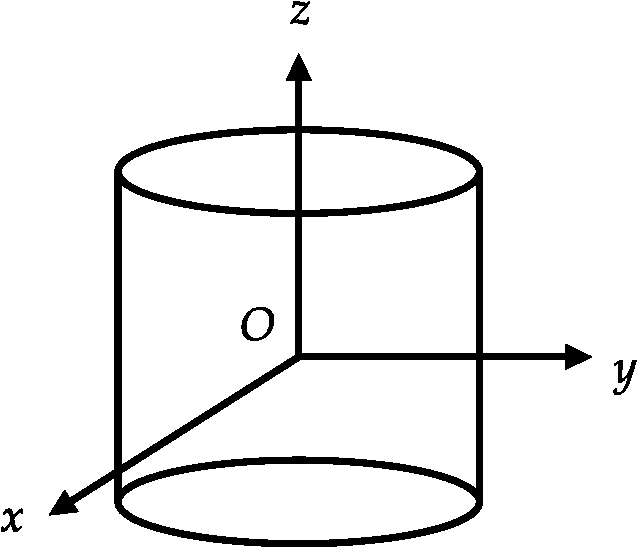
\includegraphics[height=4cm,width=4.5cm]{diagram-20210823(2)-crop}
\end{figure}
\begin{tasks}(4)
	\task[\textbf{A.}] $2 \pi a^{2}(a+h)$
	\task[\textbf{B.}] $3 \pi a^{2} h$
	\task[\textbf{C.}] $2 \pi a^{2} h$
	\task[\textbf{D.}] Zero
\end{tasks}
\item Identify the correct statement for the following vectors $\vec{a}=3 \hat{i}+2 \hat{j}$ and $\vec{b}=\hat{i}+2 \hat{j}$
{\exyear{GATE 2012}}
\begin{tasks}(1)
	\task[\textbf{A.}] The vectors $\vec{a}$ and $\vec{b}$ are linearly independent
	\task[\textbf{B.}] The vectors $\vec{a}$ and $\vec{b}$ are linearly dependent
	\task[\textbf{C.}] The vectors $\vec{a}$ and $\vec{b}$ are orthogonal
	\task[\textbf{D.}] The vectors $\vec{a}$ and $\vec{b}$ are normalized
\end{tasks}
	\item If $\vec{A}$ and $\vec{B}$ are constant vectors, then $\vec{\nabla}(\vec{A} \cdot(\vec{B} \times \vec{r}))$ is
{\exyear{GATE 2013}}

\begin{tasks}(4)
	\task[\textbf{A.}] $\vec{A} \cdot \vec{B}$
	\task[\textbf{B.}] $\vec{A} \times \vec{B}$
	\task[\textbf{C.}] $\vec{r}$
	\task[\textbf{D.}]  Zero
\end{tasks}
\item The unit vector perpendicular to the surface $x^{2}+y^{2}+z^{2}=3$ at the point $(1,1,1)$ is
{\exyear{GATE 2014}}

\begin{tasks}(4)
	\task[\textbf{A.}] $\frac{\hat{x}+\hat{y}-\hat{z}}{\sqrt{3}}$
	\task[\textbf{B.}] $\frac{\hat{x}-\hat{y}-\hat{z}}{\sqrt{3}}$
	\task[\textbf{C.}] $\frac{\hat{x}-\hat{y}+\hat{z}}{\sqrt{3}}$
	\task[\textbf{D.}] $\frac{\hat{x}+\hat{y}+\hat{z}}{\sqrt{3}}$
\end{tasks}
	\item The direction of $\vec{\nabla} f$ for a scalar field $f(x, y, z)=\frac{1}{2} x^{2}-x y+\frac{1}{2} z^{2}$ at the point $P(1,1,2)$ is
{\exyear{GATE 2016}}

\begin{tasks}(4)
	\task[\textbf{A.}] $\frac{(-\hat{j}-2 \hat{k})}{\sqrt{5}}$
	\task[\textbf{B.}] $\frac{(-\hat{j}+2 \hat{k})}{\sqrt{5}}$
	\task[\textbf{C.}] $\frac{(\hat{j}-2 \hat{k})}{\sqrt{5}}$
	\task[\textbf{D.}] $\frac{(\hat{j}+2 \hat{k})}{\sqrt{5}}$
\end{tasks}
\question In spherical polar coordinates $(r, \theta, \phi)$, the unit vector $\hat{\theta}$ at $(10, \pi / 4, \pi / 2)$ is
{\exyear{GATE 2018}}

\begin{tasks}(2)
	\task[\textbf{A.}] $\hat{k}$
	\task[\textbf{B.}] $\frac{1}{\sqrt{2}}(\hat{j}+\hat{k})$
	\task[\textbf{C.}]  $\frac{1}{\sqrt{2}}(-\hat{j}+\hat{k})$
	\task[\textbf{D.}] $\frac{1}{\sqrt{2}}(\hat{j}-\hat{k})$
\end{tasks}
\item Given $\vec{V}_{1}=\hat{i}-\hat{j}$ and $\vec{V}_{2}=-2 \hat{i}+3 \hat{j}+2 \hat{k}$, which one of the following $\vec{V}_{3}$ makes $\left(\vec{V}_{1}, \vec{V}_{2}, \vec{V}_{3}\right)$
a complete set for a three dimensional real linear vector space?
{\exyear{GATE 2018}}

\begin{tasks}(2)
	\task[\textbf{A.}] $\vec{V}_{3}=\hat{i}+\hat{j}+4 \hat{k}$
	\task[\textbf{B.}]  $\vec{V}_{3}=2 \hat{i}-\hat{j}+2 \hat{k}$
	\task[\textbf{C.}] $\vec{V}_{3}=\hat{i}+2 \hat{j}+6 \hat{k}$
	\task[\textbf{D.}] $\vec{V}_{3}=2 \hat{i}+\hat{j}+4 \hat{k}$
\end{tasks}
\end{enumerate}
\colorlet{ocre1}{ocre!70!}
\colorlet{ocrel}{ocre!30!}
\setlength\arrayrulewidth{1pt}
\begin{table}[H]
	\centering
	\arrayrulecolor{ocre}
	\begin{tabular}{|p{1.5cm}|p{1.5cm}||p{1.5cm}|p{1.5cm}|}
		\hline
		\multicolumn{4}{|c|}{\textbf{Answer key}}\\\hline\hline
		\rowcolor{ocrel}Q.No.&Answer&Q.No.&Answer\\\hline
		1&\textbf{a} &2&\textbf{d}\\\hline 
		3&\textbf{b} &4&\textbf{a} \\\hline
		5&\textbf{b} &6&\textbf{d} \\\hline
		7&\textbf{b}&8&\textbf{d}\\\hline
		9&\textbf{d}&10&\textbf{}\\\hline
		
		
	\end{tabular}
\end{table}

\newpage
\begin{abox}
Problem Set-3	
\end{abox}
\begin{enumerate}[label=\color{ocre}\textbf{\arabic*.}]
	\item Three unit vectors $\vec{a}, \vec{b}, \vec{c}\left(\vec{b}\right.$ and $\vec{c}$ are not parallel) are such that $\vec{a} \times(\vec{b} \times \vec{c})=\frac{\sqrt{3}}{2} \vec{c} .$ The
	angles which $\vec{a}$ makes with $\vec{b}$ and $\vec{c},$ respectively are
	\begin{tasks}(2)
		\task[\textbf{a.}]$30^{\circ}, 90^{\circ}$  
		\task[\textbf{b.}]$150^{\circ}, 90^{\circ}$
		\task[\textbf{c.}]$60^{\circ}, 90^{\circ}$ 
		\task[\textbf{d.}]$90^{\circ}, 30^{\circ}$ 
	\end{tasks}
	\begin{answer}
		\begin{flalign*}
		( \vec{a} \times(\vec{b} \times \vec{c})=\frac{\sqrt{3}}{2} \vec{c} &\Rightarrow \vec{b}(\vec{a} \cdot \vec{c})-\vec{c}(\vec{a} \cdot \vec{b})=\frac{\sqrt{3}}{2} \vec{c}
		\intertext{Comparing coefficients of $\vec{b}$ and $\vec{c}$ on both sides.}
		\vec{a} \cdot \vec{c}&=0 \Rightarrow \vec{a} \perp \vec{c}\\
		\vec{a} \cdot \vec{b}&=\frac{\sqrt{3}}{2} \\\Rightarrow a b \cos \theta&=-\frac{\sqrt{3}}{2}\\ \Rightarrow \cos \theta&=-\frac{\sqrt{3}}{2} \\\Rightarrow \theta&=150^{\circ}
		\intertext{The angle which $ \quad\vec{a} $ makes with $ \vec{b}  $ and $ \vec{c} $  are $ 150^{\circ} , 90^{\circ}$ respectively.Correct option is (b)}
		\end{flalign*}
	\end{answer}
\item Find the angle between the two surfaces $5 x+y+z=1$ and $3 x+3 y+3 z=5$.
\begin{tasks}(2)
	\task[\textbf{a.}]$\cos ^{-1}\left(\frac{7}{3}\right)$   
	\task[\textbf{b.}]$\cos ^{-1}\left(\frac{7}{9}\right)$ 
	\task[\textbf{c.}]$\cos ^{-1}\left(\frac{7}{27}\right)$ 
	\task[\textbf{d.}]$\cos ^{-1}\left(\frac{21}{9}\right)$ 
\end{tasks}
\begin{answer}
\begin{align*}
\text{Given}\quad\phi_{1}: 5 x+y+z=1 &\quad\text{and}\quad\phi_{2}: 3 x+3 y+3 z=5\\
\text{therefore,}\\
\cos \theta&=\frac{\vec{\nabla} \phi_{1} \cdot \vec{\nabla} \phi_{2}}{\left|\vec{\nabla} \phi_{1}\right|\left|\vec{\nabla} \phi_{2}\right|}\\&=\frac{(5 \hat{i}+\hat{j}+\hat{k}) \cdot(3 \hat{i}+3 \hat{j}+3 \hat{k})}{\sqrt{27} \cdot \sqrt{27}}\\&=\frac{21}{27} \\\Rightarrow \theta&=\cos ^{-1}\left(\frac{7}{9}\right)
\end{align*}
\end{answer}
\item The equation of the plane that is tangent to the surface $x y z=8$ at the point (1,2,4) is
\begin{tasks}(2)
	\task[\textbf{a.}]$x+2 y+4 z=12$  
	\task[\textbf{b.}]$4 x+2 y+z=12$
	\task[\textbf{c.}]$x+4 y+2=0$ 
	\task[\textbf{d.}]$x+y+z=7$ 
\end{tasks}
\begin{answer}
	\begin{align*}
	\text{To get a normal at the surface let's take the gradient}\\
		\vec{\nabla}(x y z)&=y z \hat{i}+z x \hat{j}+\hat{k} x y\\&=8 \hat{i}+4 \hat{j}+2 \hat{k}\\
		\text{We want a plane perpendicular to this so:}\\
		\left(\vec{r}-\vec{r}_{0}\right) \cdot \frac{(8 \hat{i}+4 \hat{j}+2 \hat{k})}{\sqrt{64+16+4}}&=0\\
		|(x-1) \hat{i}+(y-2) \hat{j}+(z-4) \hat{k}| \cdot[8 \hat{i}+4 \hat{j}+2 \hat{k}]&=0\\ \Rightarrow 4 x+2 y+z&=12
	\end{align*}
	
\end{answer}
\item If $\vec{A}=\hat{i} y z+\hat{j} x z+\hat{k} x y$, then the integral $\oint_{C} \vec{A} \cdot d \vec{l}$ (where $C$ is along the perimeter of a rectangular
area bounded by $x=0, x=a$ and $y=0, y=b)$ is
\begin{tasks}(4)
	\task[\textbf{a.}]$\frac{1}{2}\left(a^{3}+b^{3}\right)$  
	\task[\textbf{b.}]$\pi\left(a b^{2}+a^{2} b\right)$
	\task[\textbf{c.}]$\pi\left(a^{3}+b^{3}\right)$ 
	\task[\textbf{d.}]0 
\end{tasks}
\begin{answer}
	\begin{align*}
	\oint_{C} \vec{A} \cdot d \vec{l}&=\int_{S}(\vec{\nabla} \times \vec{A}) d \vec{a}=0 \\
	\because \vec{\nabla} \times \vec{A}&=0
	\end{align*}

\end{answer}
\item Value of the integral $\oint\left(x y d y-y^{2} d x\right)$, where $c$ is
the square cut from the quadrant by the lines $x=1$ and $y=1$ will be (use Green's theorem to change the line integral into double integral)
\begin{tasks}(4)
	\task[\textbf{a.}] $\frac{1}{2}$ 
	\task[\textbf{b.}]1
	\task[\textbf{c.}]$\frac{3}{2}$ 
	\task[\textbf{d.}]$\frac{5}{3}$ 
\end{tasks}
\begin{answer}
	\begin{align*}
 \intertext{We know that Green's theorem is given by}\oint_{c} \phi d x+\psi d y&=\iint_{R}\left(\frac{\partial \psi}{\partial x}-\frac{\partial \phi}{\partial y}\right) d x d y\\
 \text{Here,}I&=\oint\left(x y d y-y^{2} d x\right)\\&=\oint\left(-y^{2}\right) d x+(x y) d y
 \intertext{Hence, we can deduce}\phi &=-y^{2} \\
 \psi &=x y \\
 \frac{\partial \psi}{\partial x} &=y \\
 \frac{\partial \phi}{\partial y} &=-2 y
 \intertext{Substituting in Green's theorem, we get}
 I &=\int_{y=0}^{1} \int_{x=0}^{1}[y-(-2 y)] d x d y=\int_{y=0}^{1} \int_{x=0}^{1} 3 y d x d y \\
 &=\int_{y=0}^{1}[3 x y]_{x=0}^{1} d y=\int_{y=0}^{1} 3 y d y \\
 &=\frac{3}{2}
\end{align*}
Thus the correct option is (c).
\end{answer}
\item  Evaluate $\int_{C} \vec{F} \cdot \overrightarrow{d r},$ where $F=x^{2} \hat{i}+y^{3} \hat{j}$ and curve $C$ is the arc of parabola $y=x^{2}$ in the $x-y$
plane from (0,0) to (1,1) 
\begin{tasks}(2)
	\task[\textbf{a.}]$\frac{7}{12}$  
	\task[\textbf{b.}]$\frac{7}{12}$ 
	\task[\textbf{c.}]$\frac{7}{12}$  
	\task[\textbf{d.}]$\frac{7}{12}$ 
\end{tasks}
\begin{answer}
	\begin{align*}
	\text{Along the curve C,}
	y=x^{2} \Rightarrow d y=2 x d x ;\\
	\vec{r}&=x \hat{i}+x^{2} \hat{j} \Rightarrow d \vec{r}=d x \hat{i}+2 x d \hat{x} j\\
	\text { Therefore, } \int_{C} \vec{F} \cdot d \vec{r}&=\int_{x=0}^{1}\left[x^{2} d x+x^{6}(2 x) d x\right] \\
	&=\int_{0}^{1}\left(x^{2}+2 x^{7}\right) d x=\left[\frac{x^{3}}{3}+\frac{2 x^{8}}{8}\right]_{0}^{1}\\&=\frac{7}{12}
	\end{align*}
	
\end{answer}
\item At any point of the curve $x=3 \cos t, y=3 \sin t, z=4 t,$ find
The unit tangent vector 
\begin{tasks}(2)
	\task[\textbf{a.}]$\frac{1}{\sqrt 10}(-3 \sin t \hat{i}+3 \cos t \hat{j}+4 \hat{k})$   
	\task[\textbf{b.}]$\frac{1}{10}(-3 \sin t \hat{i}+3 \cos t \hat{j}+4 \hat{k})$ 
	\task[\textbf{c.}]$\frac{1}{5}(-3 \sin t \hat{i}+3 \cos t \hat{j}+4 \hat{k})$ 
	\task[\textbf{d.}]$\frac{1}{5(\sin t+\cos t)}(-3 \sin t \hat{i}+3 \cos t \hat{j}+4 \hat{k})$  
\end{tasks}
\begin{answer}
\begin{align*}
	\quad\vec{r} &=x \hat{i}+y \hat{j}+z \hat{k} \Rightarrow \vec{r}=(3 \cos t) \hat{i}+(3 \sin t) \hat{j}+(4 t) \hat{k} \\
	\frac{d \vec{r}}{d t} &=(-3 \sin t) \hat{i}+(3 \cos t) \hat{j}+4 \hat{k}\quad
	\text{which is the required tangent vector.} \intertext{Magnitude of tangent vector} &=\sqrt{(-3 \sin t)^{2}+(3 \cos t)^{2}+(4)^{2}}=5
	\intertext{Unit tangent vector}&=\frac{1}{5}(-3 \sin t \hat{i}+3 \cos t \hat{j}+4 \hat{k})
\end{align*}
\end{answer}
\item The unit normal vector of the point $\left[\frac{a}{\sqrt{3}}, \frac{b}{\sqrt{3}}, \frac{c}{\sqrt{3}}\right]$ on the surface of the ellipsoid
$\frac{x^{2}}{a^{2}}+\frac{y^{2}}{b^{2}}+\frac{z^{2}}{c^{2}}=1$ is
\begin{tasks}(2)
	\task[\textbf{a.}]$\frac{b c \hat{i}+c a \hat{j}+a b \hat{k}}{\sqrt{b^{2} c^{2}+c^{2} a^{2}+a^{2} b^{2}}}$  
	\task[\textbf{b.}]$\frac{a \hat{i}+b \hat{j}+c \hat{k}}{\sqrt{a^{2}+b^{2}+c^{2}}}$
	\task[\textbf{c.}]$\frac{b \hat{i}+c \hat{j}+a \hat{k}}{\sqrt{a^{2}+b^{2}+c^{2}}}$ 
	\task[\textbf{d.}]$\frac{\hat{i}+\hat{j}+\hat{k}}{\sqrt{3}}$ 
\end{tasks}
\begin{answer}
	\begin{align*}
	\text{Here,}\phi&=\frac{x^{2}}{a^{2}}+\frac{y^{2}}{b^{2}}+\frac{z^{2}}{c^{2}}-1\\
	\text{Unit normal vector is}\frac{\vec{\nabla} \phi}{|\vec{\nabla} \phi|}\\
	\text{So}\vec{\nabla} \phi&=\left(i \frac{\partial}{\partial x}+\hat{j} \frac{\partial}{\partial y}+\hat{k} \frac{\partial}{\partial z}\right) \cdot\left(\frac{x^{2}}{a^{2}}+\frac{y^{2}}{b^{2}}+\frac{z^{2}}{c^{2}}-1\right)\\&=\frac{2 x \hat{i}}{a^{2}}+\frac{2 y \hat{j}}{b^{2}}+\frac{2 z \hat{k}}{c^{2}}\\
	\left.\vec{\nabla} \phi\right|_{\left(\frac{a}{\sqrt{3}}, \frac{b}{\sqrt{3}}, \frac{c}{\sqrt{3}}\right)}&=\frac{2}{a \sqrt{3}} \hat{i}+\frac{2}{b \sqrt{3}} \hat{j}+\frac{2}{c \sqrt{3}} \hat{k}\\
	|\vec{\nabla} \phi|&=\sqrt{\frac{4}{3 a^{2}}+\frac{4}{3 b^{2}}+\frac{4}{3 c^{2}}}\\&=\frac{2}{\sqrt{3}} \sqrt{\frac{b^{2} c^{2}+a^{2} c^{2}+a^{2} c^{2}}{a^{2} b^{2} c^{2}}}\\
	\left.\frac{\vec{\nabla} \phi}{|\vec{\nabla} \phi|}\right|_{\left(\frac{a}{\sqrt{3}}, \frac{b}{\sqrt{3}}, \frac{c}{\sqrt{3}}\right)}&=\frac{\frac{2}{a \sqrt{3}} \hat{i}+\frac{2}{b \sqrt{3}} \hat{j}+\frac{2}{c \sqrt{3}} \hat{k}}{\frac{2}{\sqrt{3}} \frac{\sqrt{b^{2} c^{2}+c^{2} a^{2}+a^{2} b^{2}}}{a b c}}\\&=\frac{b c \hat{i}+c a \hat{j}+a b \hat{k}}{\sqrt{b^{2} c^{2}+c^{2} a^{2}+a^{2} b^{2}}}
	\end{align*}
The correct option is (a)
\end{answer}
\item For the vector field $\vec{A}=x z^{2} \hat{i}-y z^{2} \hat{j}+z\left(x^{2}-y^{2}\right) \hat{k},$ the volume integral of the divergence of $\vec{A}$
out of the region defined by $-a \leq x \leq a,-b \leq y \leq b$ and $0 \leq z \leq c$
is:
\begin{tasks}(2)
	\task[\textbf{a.}]$\frac{4}{3} a b c\left[a^{2}-b^{2}\right]$  
	\task[\textbf{b.}] $\frac{2}{3} a b c\left[a^{2}-b^{2}\right]$
	\task[\textbf{c.}]$\frac{1}{3} a b c\left[a^{2}-b^{2}\right]$ 
	\task[\textbf{d.}]$a b c\left[a^{2}-b^{2}\right]$ 
\end{tasks}
\begin{answer}
	\begin{align*}
	\text{Since,} \vec{A}&=x z^{2} \hat{i}-y z^{2} \hat{j}+z\left(x^{2}-y^{2}\right) \hat{k} \Rightarrow \vec{\nabla} \cdot \vec{A}=z^{2}-z^{2}+\left(x^{2}-y^{2}\right)=x^{2}-y^{2}\\
	\text{Thus,}\int_{V}(\vec{\nabla} \cdot \vec{A}) d \tau\\&=\int_{x=-a}^{x=+a} \int_{y=-b}^{y=+b} \int_{z=0}^{z=c}\left(x^{2}-y^{2}\right) d x d y d z\\&=\int_{y=-b}^{y=+b} \int_{z=0}^{z=c}\left[\frac{x^{3}}{3}-y^{2} x\right]_{-a}^{+a} d y d z\\&=\int_{y=-b}^{y=+b} \int_{z=0}^{z=c}\left[\frac{2}{3} a^{3}-2 a y^{2}\right] d y d z\\
	\Rightarrow \int_{V}(\vec{\nabla} \cdot \vec{A}) d \tau&=\int_{z=0}^{z=c}\left[\frac{2}{3} a^{3} y-2 a \frac{y^{3}}{3}\right]_{-b}^{+b} d z=\int_{z=0}^{z=c}\left[\frac{4}{3} a^{3} b-\frac{4}{3} a b^{3}\right] d z\\&=\frac{4}{3} a b c\left[a^{2}-b^{2}\right]
	\end{align*}
 Correct option is (a)
\end{answer}
\item The value of $\oint \vec{F} \cdot d \vec{r},$ where $C$ is the curve bounded by $x^{2}+y^{2} \geq 4 ; x^{2}+y^{2} \leq 16 ; x \geq 0$
and $\vec{F}=-y \hat{i}+x \hat{j}+z \hat{k}$ is ....
\begin{tasks}(4)
	\task[\textbf{a.}]$ 12\pi$ 
	\task[\textbf{b.}]$ 24 \pi$ 
	\task[\textbf{c.}]$ \frac{14 \pi}{3}$  
	\task[\textbf{d.}]$ \frac{10 \pi}{3}$  
\end{tasks}
\begin{answer}
\begin{align*}
\intertext{Using Stoke's theorem,}\int_{C} \vec{F} \cdot d \vec{r}&=\iint_{S}(\vec{\nabla} \times \vec{F}) \cdot d \vec{S}\\
\int_{C} \vec{F} \cdot d \vec{r}&=\iint_{S}(\vec{\nabla} \times \vec{F}) \cdot d \vec{S}\\
\vec{\nabla} \times \vec{F}&=\left|\begin{array}{ccc}
\hat{i} & \hat{j} & \hat{k} \\
\frac{\partial}{\partial x} & \frac{\partial}{\partial y} & \frac{\partial}{\partial z} \\
-y & x & z
\end{array}\right|=\hat{i}(0-0)-\hat{j}(0-0)+\hat{k}(1+1)=2 \hat{k}\end{align*}
\begin{figure}[H]
	\centering
	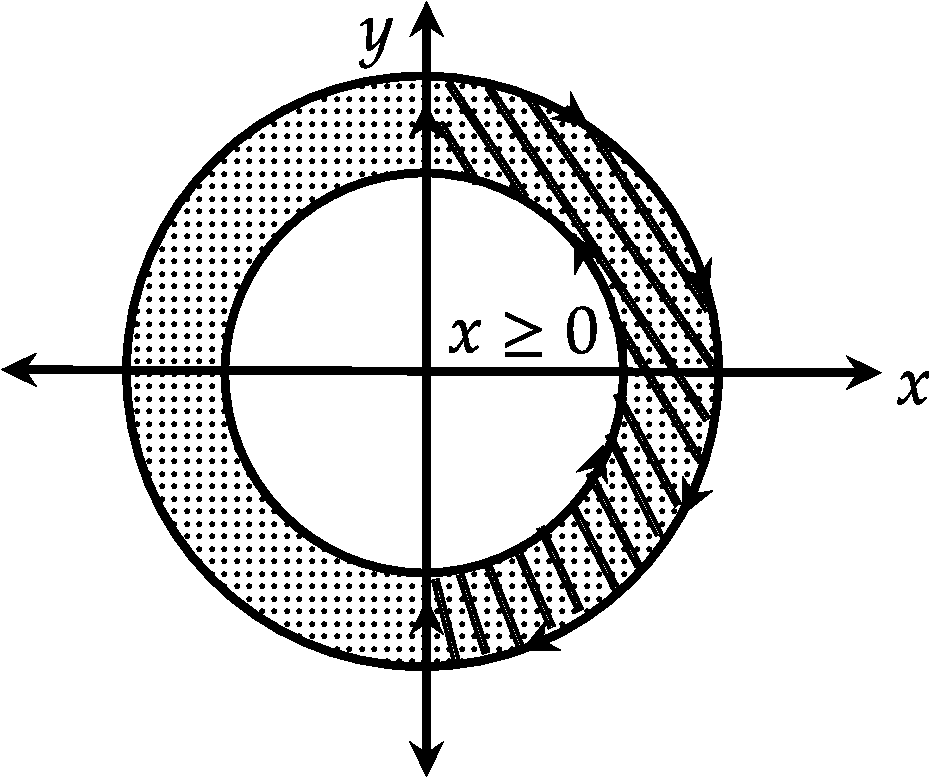
\includegraphics[height=3.5cm,width=4cm]{pset 3-10}
\end{figure}
\begin{align*}
\text { And } d \vec{S}&=d x d y \hat{k}\\
\therefore \quad \iint_{S}(\vec{\nabla} \times \vec{F}) \cdot d \vec{S}&=2 \iint d x d y\\
\intertext { Put, $ x=r \cos \theta, y=r \sin \theta $  and  $ d x d y=r d r d \theta $}
&=2 \int_{\theta=-\frac{\pi}{2}}^{\frac{\pi}{2}} \int_{r=2}^{4} r d r d \theta\\&=2\left(\frac{r^{2}}{2}\right)_{2}^{4}( \pi)= \pi \times 12=12 \pi
\end{align*}	
\end{answer}

\end{enumerate}



%\input{chapter/Practise set - 1,2 Solution}
%\chapter{Dirac Delta Function}
In mathematical models of physical systems we often come across functions that have finite or infinite discontinuities (Potential barriers, Impulse functions). Even though they dont belongs to the generalm definition of functions we can represent them as generalised function or distributions. The most common among them are the step function and the dirac delta function.
\section{The Step Function}
Let's start with the definition of the unit step function, $\theta(x)$ :
$$
\theta(x)=\left\{\begin{array}{ll}
0 & \text { for } x<0 \\
1 & \text { for } x>0
\end{array}\right.
$$
We do not define $\theta(x)$ at $x=0$. Rather, at $x=0$ we think of it as in transition between 0 and 1 .The function is called the unit step function because it takes a unit step at $x=0$. It is sometimes called the \textbf{Heaviside function}. The graph of $\theta(x)$ is simple.
It is obvious that $\theta(x)$ has a finite jump at $x=0$. It is sometimes convenient to define $\theta(0)$ to be the average value $\frac{1}{2}$, but this is not always necessary.
\begin{align*}
\text{The sum } \ \theta(x)+\theta(-x)&=1\\
\text{The difference}\ \theta(x)-\theta(-x)&=\varepsilon(x)
\end{align*}
Where, $\varepsilon(x)$ is the signum function.
\begin{equation}
\varepsilon(x)=\left\{\begin{array}{rr}
+1 & \text { for } x>0 \\
-1 & \text { for } x<0 \\
0 & \text { for } x=0
\end{array}\right.
\end{equation} The function $\varepsilon(x)$ looks like the limit of a tanh (or hyperbolic tangent) function as the 'kink' in the function becomes more and more steep, i.e., as the slope at the origin tends to infinity, as shown in Figure. In fact, we could define $\varepsilon(x)$ as the limit of a continous sequence of functions $\tanh(\frac{x}{\varepsilon(x)})$.
\section{Dirac Delta Function}
\subsection{Kronecker delta $\delta$}
let us consider a sequence $\left(a_{1}, a_{2}, \ldots\right)=\left\{a_{j} \mid j=1,2, \ldots\right\} .$ How do we select a particular member $a_{i}$ from the sequence? We do so by summing over all members of the sequence with a selector called the \textbf{Kronecker delta}, denoted by $\delta_{i j}$ and defined as
$\delta_{i j} \stackrel{\text { def. }}{=}\left\{\begin{array}{ll}1 & \text { if } i=j \\ 0 & \text { if } i \neq j\end{array}\right.$
It follows immediately that
\begin{align*}
\sum_{j} \delta_{i j} a_{j}&=a_{i}\\
\sum_{j} \delta_{i j}&=a_{i}\qquad \text{For each value of } \ i\\
\delta_{i j}&=\delta_{j i} \qquad \text{Symmetry property. }
\end{align*}
Now if  we have a continuos function, we must replace the summation over$j$ by an integration over $x$


%\chapter{Power series Solution and Special functions}
\section{Series Solution Method}
Series expansion is a  method of obtaining one solution of the linear, second-order, homogeneous ODE. The method, will always work, provided the point of expansion is no worse than a regular singular point.In physics this very gentle condition is almost always satisfied. 
A linear, second-order, homogeneous ODE can be written in the form
\begin{equation}
\frac{d^{2} y}{d x^{2}}+P(x) \frac{d y}{d x}+Q(x) y=0 \label{DE002}
\end{equation}
The most general solution of the equation \ref{DE002} may be written as,
\begin{equation}
y(x)=c_{1} y_{1}(x)+c_{2} y_{2}(x)
\end{equation}
But a physical problem may lead to a nonhomogeneous, linear, second-order ODE
\begin{equation}
\frac{d^{2} y}{d x^{2}}+P(x) \frac{d y}{d x}+Q(x) y=F(x)\label{DE003}
\end{equation}
Hence the most general solution to the equation \label{DE003} will be of the form,
\begin{equation}
y(x)=c_{1} y_{1}(x)+c_{2} y_{2}(x)+y_{p}(x)
\end{equation}
The constants $c_{1}$ and $c_{2}$ will eventually be fixed by boundary conditions.\\\\
There are two series solution method  for differential equation,
\begin{enumerate}
	\item \textbf{Simple series expansion method}
	\item \textbf{Frobenious Method}
\end{enumerate}
\subsection{Simple Power Series Expansion Method}
The simple series expansion method works for differential equations whose solutions are well-behaved at the expansion point $x = 0$.
This method can be illustrated by Linear classical oscillator problem
\subsection{Classical Linear Oscillator}
\begin{align}
\frac{d^{2} y}{d x^{2}}+\omega^{2} y&=0 \label{DE003}\\
\text{with known solutions} \ y&=\sin \omega x, \cos \omega x\\
\text{We try}\ y(x) &=x^{k}\left(a_{0}+a_{1} x+a_{2} x^{2}+a_{3} x^{3}+\cdots\right) \\
&=\sum_{\lambda=0}^{\infty} a_{\lambda} x^{k+\lambda}, \quad a_{0} \neq 0 \label{DE004}\\
\intertext{with the exponent $k$ and all the coefficients $a_{\lambda}$ still undetermined. Note that $k$ need not be an integer. By differentiating twice, we obtain}
\frac{d y}{d x} &=\sum_{\lambda=0}^{\infty} a_{\lambda}(k+\lambda) x^{k+\lambda-1} \\
\frac{d^{2} y}{d x^{2}} &=\sum_{\lambda=0}^{\infty} a_{\lambda}(k+\lambda)(k+\lambda-1) x^{k+\lambda-2}
\intertext{By substituting into equation.\ref{DE003}, we have}
\sum_{\lambda=0}^{\infty} a_{\lambda}(k+\lambda)(k+\lambda-1) x^{k+\lambda-2}+\omega^{2} \sum_{\lambda=0}^{\infty} a_{\lambda} x^{k+\lambda}&=0 \label{DE005}
\intertext{The coefficients of each power of $x$ on the left-hand side of equation.\ref{DE005} must vanish individually.The lowest power of $x$ appearing in equation.\ref{DE005} is $x^{k-2}$, for $\lambda=0$ in the first summation. The requirement that the coefficient vanish  yields,}
a_{0} k(k-1)&=0
\intertext{We had chosen $a_{0}$ as the coefficient of the lowest nonvanishing terms of the series \ref{DE004}, hence, by definition, $a_{0} \neq 0$. Therefore we have,}
k(k-1)&=0 \label{DE006}
\end{align}
\textbf{This equation, coming from the coefficient of the lowest power of $x$, we call the {indicial equation}.} The indicial equation and its roots are of critical importance to our analysis.
\\From equation.\ref{DE006}, \qquad $k=0 $ or $k=1$\\
The only way a power series can be zero is, it's coefficients must be equal to zero. But here the power of $x$ in the equation do not match up. The Coefficent of $x$ in the first term is,${k+\lambda-2} $ and for the second term it is,$k+\lambda$, to make them equal, we can replace $\lambda$ by $\lambda+2$ in the first term. Then we get,
\begin{align}
\sum_{\lambda=2}^{\infty} a_{\lambda+2}(k+\lambda+2)(k+\lambda+1) x^{k+\lambda}+\omega^{2} \sum_{\lambda=0}^{\infty} a_{\lambda} x^{k+\lambda}&=0\\
\sum_{\lambda=2}^{\infty} a_{\lambda+2}(k+\lambda+2)(k+\lambda+1) +\omega^{2} \sum_{\lambda=0}^{\infty} a_{\lambda} &=0
\intertext{Here the coefficients  are independent summations and $\lambda $ is a dummy index. Then we get,}
a_{\lambda+2}(k+\lambda+2)(k+\lambda+1) +\omega^{2} a_{\lambda} &=0\\
a_{\lambda+2}&=-a_{\lambda} \frac{\omega^{2}}{(k+\lambda+2)(k+\lambda+1)}\label{DE007}
\end{align}
For this example, if we start with $a_{0}$, Equation.\ref{DE007} leads to the even coefficients $a_{2}, a_{4}$, and so on, and ignores $a_{1}, a_{3}, a_{5}$, and so on. Since $a_{1}$ is arbitrary if $k=0$ and necessarily zero if $k=1$, 
$$
a_{3}=a_{5}=a_{7}=\cdots=0
$$
and all the odd-numbered coefficients vanish. The odd powers of $x$ will actually reappear when the second root of the indicial equation is used.
\begin{align}
a_{\lambda+2}&=-a_{\lambda} \frac{\omega^{2}}{(\lambda+2)(\lambda+1)}
\intertext{which leads to}
a_{2}&=-a_{0} \frac{\omega^{2}}{1 \cdot 2}=-\frac{\omega^{2}}{2 !} a_{0} \\
a_{4}&=-a_{2} \frac{\omega^{2}}{3 \cdot 4}=+\frac{\omega^{4}}{4 !} a_{0} \\
a_{6}&=-a_{4} \frac{\omega^{2}}{5 \cdot 6}=-\frac{\omega^{6}}{6 !} a_{0}, \quad \text { and so on. }
\intertext{By inspection (and mathematical induction),}
a_{2 n}&=(-1)^{n} \frac{\omega^{2 n}}{(2 n) !} a_{0}
\intertext{and our solution is}
y(x)_{k=0}&=a_{0}\left[1-\frac{(\omega x)^{2}}{2 !}+\frac{(\omega x)^{4}}{4 !}-\frac{(\omega x)^{6}}{6 !}+\cdots\right]\\&=a_{0} \cos \omega x\\
\intertext{If we choose the indicial equation root $k=1$ Equation.\ref{DE007}, the recurrence relation becomes}
a_{j+2}&=-a_{j} \frac{\omega^{2}}{(j+3)(j+2)}\\
\intertext{Substituting in $j=0,2,4$, successively, we obtain}
a_{2}=-a_{0} \frac{\omega^{2}}{2 \cdot 3}&=-\frac{\omega^{2}}{3 !} a_{0} \\
a_{4}=-a_{2} \frac{\omega^{2}}{4 \cdot 5}&=+\frac{\omega^{4}}{5 !} a_{0} \\
a_{6}=-a_{4} \frac{\omega^{2}}{6 \cdot 7}&=-\frac{\omega^{6}}{7 !} a_{0}, \quad \text { and so on. }
\intertext{Again, by inspection and mathematical induction,}
a_{2 n}&=(-1)^{n} \frac{\omega^{2 n}}{(2 n+1) !} a_{0}\\
\intertext{For this choice, $k=1$, we obtain}
y(x)_{k=1} &=a_{0} x\left[1-\frac{(\omega x)^{2}}{3 !}+\frac{(\omega x)^{4}}{5 !}-\frac{(\omega x)^{6}}{7 !}+\cdots\right] \\
&=\frac{a_{0}}{\omega}\left[(\omega x)-\frac{(\omega x)^{3}}{3 !}+\frac{(\omega x)^{5}}{5 !}-\frac{(\omega x)^{7}}{7 !}+\cdots\right] \\
&=\frac{a_{0}}{\omega} \sin \omega x
\end{align}
\subsubsection{Power Series Solution (About an Ordinary Point)}
Find the power series solution of $\left(1-x^{2}\right) y^{\prime \prime}-2 x y^{\prime}+2 y=0$ about $x=0$\\\\
Since $x=0$ is an ordinary point of the given differential equation, the solution can be written as
\begin{align*}
y&=\sum_{k=0}^{\infty} a_{k} x^{k} \\ \frac{d y}{d x}&=\sum_{k=0}^{\infty} k a_{k} x^{k-1} \\ \frac{d^{2} y}{d x^{2}}&=\sum_{k=0}^{\infty} a_{k} k(k-1) x^{k-2}
\intertext{Substituting these values in the given equation we get,}
\left(1-x^{2}\right) \sum_{k} a_{k} k(k-1) x^{k-2}&-2 x \sum_{k} a_{k}(k) x^{k-1}+2 \sum_{k} a_{k} x^{k}=0 \\
\sum_{k=2} a_{k} k(k-1) x^{k-2}&-\sum\left(k^{2}+k-2\right) a_{k} x^{k}=0
\intertext{now equating the coefficient of $x^{k}$ then}
(k+2)(k+1) a_{k+2}-\left(k^{2}+k-2\right) a_{k}&=0 \\a_{k+2}&=\frac{k-1}{(k+1)} a_{k}\\
\text{For} \ k&=0 \Rightarrow a_{2}=-a_{0} \\ k&=1 \Rightarrow a_{3}=0 \\
k&=2 \Rightarrow a_{4}=\frac{a_{2}}{3}=\frac{-a_{0}}{3}  \\ k&=3 \Rightarrow a_{5}=\frac{2}{4} a_{3}=0\\
\text{Therefore, solution}\ y&=a_{0}+a_{1} x+a_{2} x^{2}+\ldots \ldots\\&=a_{0}\left[1-x^{2}-\frac{x^{4}}{3} \ldots . .\right]+a_{1} x
\end{align*}
\subsection{Frobenious Method}
Even though the simple power series expansion method works for many functions there are some whose behaviour  precludes the simple series method like the Bessel's function. The need of Frobenious method  lies under the fact that, \textbf{any functions involving negative or fractional powers would not be amenable to power series solution method}. The Frobenious method extends the simple power series solution method to include negative and fractional powers, and it also allows a natural extension involving logarithm terms.\\
The basic idea of the Frobenius method is to look for solutions of the form
\begin{align*}
y(x) &=a_{0} x^{\lambda}+a_{1} x^{\lambda+1}+a_{2} x^{\lambda+2}+a_{3} x^{\lambda+3}+\ldots \\
&=x^{\lambda}\left(a_{0}+a_{1} x+a_{2} x^{2}+a_{3} x^{3}+\ldots\right) \\
&=x^{\lambda} \sum_{k=0}^{\infty} a_{k} x^{k} \\
&= \sum_{k=0}^{\infty} a_{k} x^{k+\lambda}
\end{align*}
The extension of the simple power series method is all in the factor $x^{\lambda}$. The power $c$ must now be determined, as well as the coefficients $a_{k}$. Since $\lambda$ may be negative, positive, and possibly non-integral, this extends considerably the range of functions which may be treated. Note that $a_{0}$ is the lowest non-zero coefficient, so by definition it cannot be zero.
\subsection{Bessel Function}
\newpage
\begin{abox}
	Problem Set -1
\end{abox}
\begin{enumerate}[label=\color{ocre}\textbf{\arabic*.}]
	\item  Let $p_{n}(x)$ (where $n=0,1,2, \ldots \ldots$ ) be a polynomial of degree $n$ with real coefficients, defined in the interval $2 \leq n \leq 4$. If $\int_{2}^{4} p_{n}(x) p_{m}(x) d x=\delta_{n m}$, then
	{\exyear{NET/JRF(JUNE-2011)}}
	\begin{tasks}(2)
		\task[\textbf{A.}] $p_{0}(x)=\frac{1}{\sqrt{2}}$ and $p_{1}(x)=\sqrt{\frac{3}{2}}(-3-x)$
		\task[\textbf{B.}]  $p_{0}(x)=\frac{1}{\sqrt{2}}$ and $p_{1}(x)=\sqrt{3}(3+x)$
		\task[\textbf{C.}] $p_{0}(x)=\frac{1}{2}$ and $p_{1}(x)=\sqrt{\frac{3}{2}}(3-x)$
		\task[\textbf{D.}] $p_{0}(x)=\frac{1}{\sqrt{2}}$ and $p_{1}(x)=\sqrt{\frac{3}{2}}(3-x)$
	\end{tasks}
	\item  The generating function $F(x, t)=\sum_{n=0}^{\infty} P_{n}(x) t^{n}$ for the Legendre polynomials $P_{n}(x)$ is $F(x, t)=\left(1-2 x t+t^{2}\right)^{-1 / 2}$. The value of $P_{3}(-1)$ is
	{\exyear{NET/JRF(DEC-2011)}}
	\begin{tasks}(4)
		\task[\textbf{A.}] $5 / 2$
		\task[\textbf{B.}] $3 / 2$
		\task[\textbf{C.}] $+1$
		\task[\textbf{D.}] $-1$
	\end{tasks}
	\item  The graph of the function $f(x)$ shown below is best described by
	{\exyear{NET/JRF(DEC-2012)}}
	\begin{figure}[H]
		\centering
		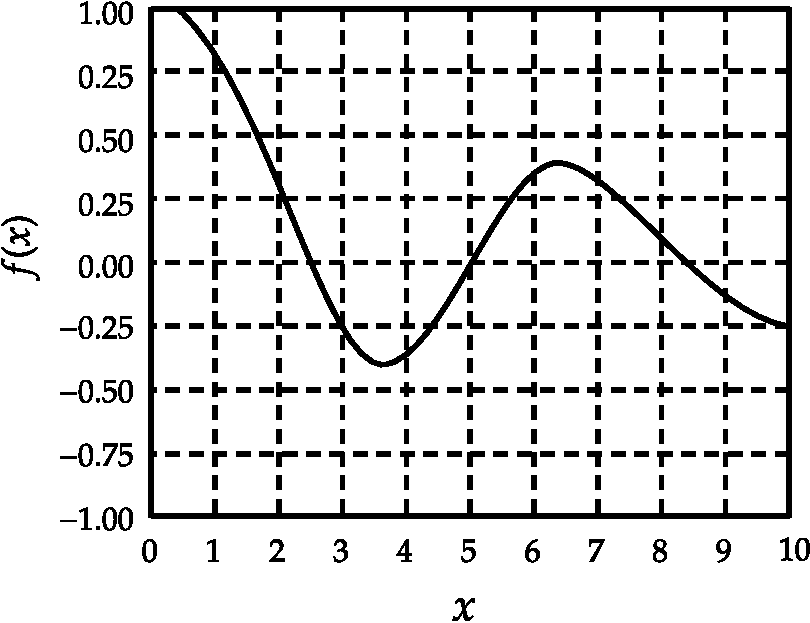
\includegraphics[height=6cm,width=8cm]{diagram-20211005(12)-crop}
	\end{figure}
	\begin{tasks}(2)
		\task[\textbf{A.}]  The Bessel function $J_{0}(x)$
		\task[\textbf{B.}] $\cos x$
		\task[\textbf{C.}] $e^{-x} \cos x$
		\task[\textbf{D.}] $\frac{1}{x} \cos x$
	\end{tasks}
	\item Given that $\sum_{n=0}^{\infty} H_{n}(x) \frac{t^{n}}{n !}=e^{-t^{2}+2 t x}$ the value of $H_{4}(0)$ is
	{\exyear{NET/JRF(JUNE-2013)}}
	\begin{tasks}(4)
		\task[\textbf{A.}] 12
		\task[\textbf{B.}] 6
		\task[\textbf{C.}] 24
		\task[\textbf{D.}] $-6$
	\end{tasks}
	\item   Given $\sum_{n=0}^{\infty} P_{n}(x) t^{n}=\left(1-2 x t+t^{2}\right)^{-1 / 2}$, for $|t|<1$, the value of $P_{5}(-1)$ is
	{\exyear{NET/JRF(JUNE-2014)}}
	\begin{tasks}(4)
		\task[\textbf{A.}] $0.26$
		\task[\textbf{B.}] 1
		\task[\textbf{C.}] $0.5$
		\task[\textbf{D.}] $-1$
	\end{tasks}
	\item The function $f(x)=\sum_{n=0}^{\infty} \frac{(-1)^{n}}{n !(n+1) !}\left(\frac{x}{2}\right)^{2 n+1}$, satisfies the differential equation
	{\exyear{NET/JRF(DEC-2014)}}
	\begin{tasks}(2)
		\task[\textbf{A.}]  $x^{2} \frac{d^{2} f}{d x^{2}}+x \frac{d f}{d x}+\left(x^{2}+1\right) f=0$
		\task[\textbf{B.}]  $x^{2} \frac{d^{2} f}{d x^{2}}+2 x \frac{d f}{d x}+\left(x^{2}-1\right) f=0$
		\task[\textbf{C.}] $x^{2} \frac{d^{2} f}{d x^{2}}+x \frac{d f}{d x}+\left(x^{2}-1\right) f=0$
		\task[\textbf{D.}] $x^{2} \frac{d^{2} f}{d x^{2}}-x \frac{d f}{d x}+\left(x^{2}-1\right) f=0$
	\end{tasks}
	\item
	 The Hermite polynomial $H_{n}(x)$, satisfies the differential equation
	$$
	\frac{d^{2} H_{n}}{d x^{2}}-2 x \frac{d H_{n}}{d x}+2 n H_{n}(x)=0
	$$
	The corresponding generating function $G(t, x)=\sum_{n=0}^{\infty} \frac{1}{n !} H_{n}(x) t^{n}$, satisfies the equation
	{\exyear{NET/JRF(DEC-2015)}}
	\begin{tasks}(2)
		\task[\textbf{A.}] $\frac{\partial^{2} G}{\partial x^{2}}-2 x \frac{\partial G}{\partial x}+2 t \frac{\partial G}{\partial t}=0$
		\task[\textbf{B.}] $\frac{\partial^{2} G}{\partial x^{2}}-2 x \frac{\partial G}{\partial x}-2 t^{2} \frac{\partial G}{\partial t}=0$
		\task[\textbf{C.}] $\frac{\partial^{2} G}{\partial x^{2}}-2 x \frac{\partial G}{\partial x}+2 \frac{\partial G}{\partial t}=0$
		\task[\textbf{D.}]  $\frac{\partial^{2} G}{\partial x^{2}}-2 x \frac{\partial G}{\partial x}+2 \frac{\partial^{2} G}{\partial x \partial t}=0$
	\end{tasks}
	\item A stable asymptotic solution of the equation $x_{n+1}=1+\frac{3}{1+x_{n}}$ is $x=2$. If we take $x_{n}=2+\epsilon_{n}$ and $x_{n+1}=2+\epsilon_{n+1}$, where $\epsilon_{n}$ and $\epsilon_{n+1}$ are both small, the ratio $\frac{\epsilon_{n+1}}{\epsilon_{n}}$ is approximately
	{\exyear{NET/JRF(DEC-2016)}}
	\begin{tasks}(4)
		\task[\textbf{A.}] $-\frac{1}{2}$
		\task[\textbf{B.}] $-\frac{1}{4}$
		\task[\textbf{C.}]  $-\frac{1}{3}$
		\task[\textbf{D.}] $-\frac{2}{3}$
	\end{tasks}
	\item  The Green's function satisfying
	$$
	\frac{d^{2}}{d x^{2}} g\left(x, x_{0}\right)=\delta\left(x-x_{0}\right)
	$$
	with the boundary conditions $g\left(-L, x_{0}\right)=0=g\left(L, x_{0}\right)$, is
	{\exyear{NET/JRF(JUNE-2017)}}
	\begin{tasks}(1)
		\task[\textbf{A.}] $\left\{\begin{array}{ll}\frac{1}{2 L}\left(x_{0}-L\right)(x+L), & -L \leq x<x_{0} \\ \frac{1}{2 L}\left(x_{0}+L\right)(x-L), & x_{0} \leq x \leq L\end{array}\right.$
		\task[\textbf{B.}]  $\left\{\begin{array}{ll}\frac{1}{2 L}\left(x_{0}+L\right)(x+L), & -L \leq x<x_{0} \\ \frac{1}{2 L}\left(x_{0}-L\right)(x-L), & x_{0} \leq x \leq L\end{array}\right.$
		\task[\textbf{C.}] $\left\{\begin{array}{ll}\frac{1}{2 L}\left(L-x_{0}\right)(x+L), & -L \leq x<x_{0} \\ \frac{1}{2 L}\left(x_{0}+L\right)(L-x), & x_{0} \leq x \leq L\end{array}\right.$
		\task[\textbf{D.}] $\frac{1}{2 L}(x-L)(x+L), \quad-L \leq x \leq L$
	\end{tasks}
	\item  The generating function $G(t, x)$ for the Legendre polynomials $P_{n}(t)$ is
	$$
	G(t, x)=\frac{1}{\sqrt{1-2 x t+x^{2}}}=\sum_{n=0}^{\infty} x^{n} P_{n}(t), \text { for }|x|<1
	$$
	If the function $f(x)$ is defined by the integral equation $\int_{0}^{x} f\left(x^{\prime}\right) d x^{\prime}=x G(1, x)$, it can be expressed as
	{\exyear{NET/JRF(DEC-2017)}}
	\begin{tasks}(2)
		\task[\textbf{A.}] $\sum_{n, m=0}^{\infty} x^{n+m} P_{n}(1) P_{m}\left(\frac{1}{2}\right)$
		\task[\textbf{B.}] $\sum_{n, m=0}^{\infty} x^{n+m} P_{n}(1) P_{m}(1)$
		\task[\textbf{C.}] $\sum_{n, m=0}^{\infty} x^{n-m} P_{n}(1) P_{m}(1)$
		\task[\textbf{D.}] $\sum_{n, m=0}^{\infty} x^{n-m} P_{n}(0) P_{m}(1)$
	\end{tasks}
	\item In the function $P_{n}(x) e^{-x^{2}}$ of a real variable $x, P_{n}(x)$ is polynomial of degree $n$. The maximum number of extrema that this function can have is
	{\exyear{NET/JRF(JUNE-2018)}}
	\begin{tasks}(4)
		\task[\textbf{A.}] $n+2$
		\task[\textbf{B.}]  $n-1$
		\task[\textbf{C.}] $n+1$
		\task[\textbf{D.}] $n$
	\end{tasks}
	\item  The Green's function $G\left(x, x^{\prime}\right)$ for the equation $\frac{d^{2} y(x)}{d x^{2}}+y(x)=f(x)$, with the boundary values $y(0)=y\left(\frac{\pi}{2}\right)=0$, is
	{\exyear{NET/JRF(JUNE-2018)}}
	\begin{tasks}(1)
		\task[\textbf{A.}] $G\left(x, x^{\prime}\right)=\left\{\begin{array}{ll}x\left(x^{\prime}-\frac{\pi}{2}\right), & 0<x<x^{\prime}<\frac{\pi}{2} \\ \left(x-\frac{\pi}{2}\right) x^{\prime}, & 0<x^{\prime}<x<\frac{\pi}{2}\end{array}\right.$
		\task[\textbf{B.}] $G\left(x, x^{\prime}\right)=\left\{\begin{array}{ll}-\cos x^{\prime} \sin x, & 0<x<x^{\prime}<\frac{\pi}{2} \\ -\sin x^{\prime} \cos x, & 0<x^{\prime}<x<\frac{\pi}{2}\end{array}\right.$
		\task[\textbf{C.}] $G\left(x, x^{\prime}\right)=\left\{\begin{array}{ll}\cos x^{\prime} \sin x, & 0<x<x^{\prime}<\frac{\pi}{2} \\ \sin x^{\prime} \cos x, & 0<x^{\prime}<x<\frac{\pi}{2}\end{array}\right.$
		\task[\textbf{D.}] $G\left(x, x^{\prime}\right)=\left\{\begin{array}{ll}x\left(\frac{\pi}{2}-x^{\prime}\right), & 0<x<x^{\prime}<\frac{\pi}{2} \\ x^{\prime}\left(\frac{\pi}{2}-x\right), & 0<x^{\prime}<x<\frac{\pi}{2}\end{array}\right.$
	\end{tasks}
	\item The polynomial $f(x)=1+5 x+3 x^{2}$ is written as linear combination of the Legendre polynomials
	$\left(P_{0}(x)=1, P_{1}(x), P_{2}(x)=\frac{1}{2}\left(3 x^{2}-1\right)\right)$ as $f(x)=\sum_{n} c_{n} P_{n}(x)$. The value of $c_{0}$ is
	{\exyear{NET/JRF(DEC-2018)}}
	\begin{tasks}(4)
		\task[\textbf{A.}] $\frac{1}{4}$
		\task[\textbf{B.}] $\frac{1}{2}$
		\task[\textbf{C.}]  2
		\task[\textbf{D.}]  4
	\end{tasks}
	\item The Green's function $G\left(x, x^{\prime}\right)$ for the equation $\frac{d^{2} y(x)}{d x^{2}}=f(x)$, with the boundary values $y(0)=0$ and $y(1)=0$, is
	{\exyear{NET/JRF(DEC-2018)}}
	\begin{tasks}(1)
		\task[\textbf{A.}] $G\left(x, x^{\prime}\right)=\left\{\begin{array}{ll}\frac{1}{2} x\left(1-x^{\prime}\right), & 0<x<x^{\prime}<1 \\ \frac{1}{2} x^{\prime}(1-x) & 0<x^{\prime}<x<1\end{array}\right.$
		\task[\textbf{B.}] $G\left(x, x^{\prime}\right)=\left\{\begin{array}{ll}x\left(x^{\prime}-1\right), & 0<x<x^{\prime}<1 \\ x^{\prime}(1-x) & 0<x^{\prime}<x<1\end{array}\right.$
		\task[\textbf{C.}] $G\left(x, x^{\prime}\right)=\left\{\begin{array}{ll}-\frac{1}{2} x\left(1-x^{\prime}\right), & 0<x<x^{\prime}<1 \\ \frac{1}{2} x^{\prime}(1-x) & 0<x^{\prime}<x<1\end{array}\right.$
		\task[\textbf{D.}]  $G\left(x, x^{\prime}\right)=\left\{\begin{array}{ll}x\left(x^{\prime}-1\right), & 0<x<x^{\prime}<1 \\ x^{\prime}(x-1) & 0<x^{\prime}<x<1\end{array}\right.$
	\end{tasks}
	\item  The Green's function for the differential equation $\frac{d^{2} x}{d t^{2}}+x=f(t)$, satisfying the initial conditions $x(0)=\frac{d x}{d t}(0)=0$ is\\
	$$G(t, \tau)=\left\{\begin{array}{ll}0 & \text { for } \quad 0<t<\tau \\ \sin (t-\tau) & \text { for } \quad t>\tau\end{array}\right.$$\\
	The solution of the differential equation when the source $f(t)=\theta(t)$ (the Heaviside step function) is
	{\exyear{NET/JRF(JUNE-2020)}}
	\begin{tasks}(4)
		\task[\textbf{A.}] $\sin t$
		\task[\textbf{B.}] $1-\sin t$
		\task[\textbf{C.}] $1-\cos t$
		\task[\textbf{D.}] $\cos ^{2} t-1$
	\end{tasks}
\end{enumerate}
 \colorlet{ocre1}{ocre!70!}
\colorlet{ocrel}{ocre!30!}
\setlength\arrayrulewidth{1pt}
\begin{table}[H]
	\centering
	\arrayrulecolor{ocre}
	\begin{tabular}{|p{1.5cm}|p{1.5cm}||p{1.5cm}|p{1.5cm}|}
		\hline
		\multicolumn{4}{|c|}{\textbf{Answer key}}\\\hline\hline
		\rowcolor{ocrel}Q.No.&Answer&Q.No.&Answer\\\hline
		1&\textbf{D} &2&\textbf{D}\\\hline 
		3&\textbf{A} &4&\textbf{A} \\\hline
		5&\textbf{D} &6&\textbf{C} \\\hline
		7&\textbf{A}&8&\textbf{C}\\\hline
		9&\textbf{A}&10&\textbf{B}\\\hline
		11&\textbf{C} &12&\textbf{B}\\\hline
		13&\textbf{C}&14&\textbf{D}\\\hline
		15&\textbf{C}& &\\\hline
		
	\end{tabular}
\end{table}
\begin{abox}
	Problem Set -3
\end{abox}
\begin{enumerate}[label=\color{ocre}\textbf{\arabic*.}]
	\item Green function for time dependent Schrödinger wave equation is defined as $G\left(\vec{r}, t: r^{\prime}, t^{\prime}\right)$. If $H$ is Hamiltonion of system then $G\left(\vec{r}, t: r^{\prime}, t^{\prime}\right)$ will satisfied the equation
	 \begin{tasks}(1)
		\task[\textbf{a.}]$\left(i \hbar \frac{\partial}{\partial t}-H\right) G\left(\vec{r}, t ; \vec{r}^{\prime}, t^{\prime}\right)=0$
		\task[\textbf{b.}]$\left(i \hbar \frac{\partial}{\partial t}-H\right) G\left(\vec{r}, t ; \vec{r}^{\prime}, t^{\prime}\right)=\delta\left(\vec{r}-\vec{r}^{\prime}\right)$
		\task[\textbf{c.}] $\left(i \hbar \frac{\partial}{\partial t}-H\right) G\left(\vec{r}, t ; \vec{r}^{\prime}, t^{\prime}\right)=\delta\left(t-t^{\prime}\right)$
		\task[\textbf{d.}]  $\left(i \hbar \frac{\partial}{\partial t}-H\right) G\left(\vec{r}, t ; \vec{r}^{\prime}, t^{\prime}\right)=\delta\left(\vec{r}-\vec{r}^{\prime}\right) \delta\left(t-t^{\prime}\right)$
	\end{tasks}
\begin{answer}
So the correct answer is \textbf{Option (d)}
\end{answer}
	\item $G\left(x, x_{0}\right)$ is the Green's function associated with the boundary value problem consisting of ordinary differential equation.
	$$
	\frac{d}{d x}\left(p(x) \frac{d u}{d x}\right)=f(x) \text { with } u(0)=0, u(L)=0
	$$
	The discontinuity condition on the derivative $\frac{d G\left(x, x_{0}\right)}{d x}$ at $x=x_{0}$ is
	 \begin{tasks}(4)
		\task[\textbf{a.}]0
		\task[\textbf{b.}]$p\left(x_{0}\right)$
		\task[\textbf{c.}]1
		\task[\textbf{d.}] $\frac{1}{p\left(x_{0}\right)}$
	\end{tasks}
\begin{answer}
	\begin{align*}
	\left.\frac{d G}{d x}\right|_{x=x_{0}^{+}}-\left.\frac{d G}{d x}\right|_{x=x_{i 1}^{-}}=\frac{1}{p\left(x_{0}\right)}
	\end{align*}
	So the correct answer is \textbf{Option (d)}
\end{answer}
\item Consider the steady state heat equation $\frac{d^{2} u}{d x^{2}}=f(x)$ with boundary condition,
$$
u(0)=0, u(L)=0
$$
The Green's function associated with the above equation
 \begin{tasks}(2)
	\task[\textbf{a.}]Constant
	\task[\textbf{b.}] Linear function
	\task[\textbf{c.}] Parabolic function
	\task[\textbf{d.}] Hyperbolic function
\end{tasks}
\begin{answer}
	\begin{align*}
	\intertext{The Green's function satisfies}
	\frac{d^{2} G\left(x, x_{0}\right)}{d x^{2}}&=\delta\left(x-x_{0}\right)\\
\text{	with }G\left(0, x_{0}\right)&=0\text{ and }G\left(L, x_{0}\right)=0
\intertext{Corresponding homogeneous equation is:}
\frac{d^{2} G}{d x^{2}}&=0\\
\text{Solution for }x \neq x_{0}&\text{ are, }G\left(x, x_{0}\right)= \begin{cases}a+b x_{2} & x<x_{1+} \\ c+d x, & x>x_{0}\end{cases}
	\end{align*}
		So the correct answer is \textbf{Option (b)}
\end{answer}
\item Consider the steady state heat equation $\frac{d^{2} u}{d x^{2}}=f(x)$ with boundary condition. $u(0)=0, u(L)=0$
The Green's function associated with the above equation is
 \begin{tasks}(1)
	\task[\textbf{a.}] $G\left(x, x_{0}\right)= \begin{cases}\frac{x}{L}\left(x_{0}-L\right), & 0 \leq x \leq x_{0} \\ \frac{x_{0}}{L}(x-L), & x_{0} \leq x \leq L\end{cases}$
	\task[\textbf{b.}] $G\left(x, x_{0}\right)= \begin{cases}\frac{x}{L}\left(L-x_{0}\right), & 0 \leq x \leq x_{0} \\ \frac{x_{0}}{L}(L-x), & x_{0} \leq x \leq L\end{cases}$
	\task[\textbf{c.}] $G\left(x, x_{0}\right)= \begin{cases}\sqrt{\frac{x}{L},} &\quad 0 \leq x \leq x_{0} \\ \sqrt{\frac{(x-L)}{L}}, & \quad x_{0} \leq x \leq L\end{cases}$
	\task[\textbf{d.}] $G\left(x, x_{0}\right)= \begin{cases}\sqrt{\frac{L-x}{L},}, & 0 \leq x \leq x_{0} \\ \sqrt{\frac{(x)}{L}}, & x_{0} \leq x \leq L\end{cases}$
\end{tasks}
\begin{answer}
	\begin{align*}
	\intertext{The Green's function satisfies}
	\frac{d^{2} G\left(x, x_{0}\right)}{d x^{2}}&=\delta\left(x-x_{0}\right)\\
	\text{with }G\left(0, x_{0}\right)&=0\text{ and }G\left(L, x_{0}\right)=0
	\intertext{Corresponding homogeneous equation is:}
	\frac{d^{2} G}{d x^{2}}&=0\\
	\text{Solution for }&x \neq x_{0}\text{ are}\\
	G\left(x, x_{0}\right)&= \begin{cases}a+b x, & x<x_{0} \\ c+d x, & x>x_{0}\end{cases}
	\intertext{From boundary conditions:}
	G\left(0, x_{0}\right)&=0 \Rightarrow a=0\\
	G\left(L, x_{0}\right)&=0 \Rightarrow c=-d L\\
	\therefore G\left(x, x_{0}\right)&= \begin{cases}b x, & x<x_{0} \\ d(x-L), & x>x_{0}\end{cases}\\
	\text{From continuity of }&\text{Green's function at }x=x_{0},\text{ we have}\\
	b x_{0}&=d\left(x_{0}-L\right)\\
	b&=\frac{d\left(x_{0}-L\right)}{x_{0}}\\
	\text{From discontinuity of }&\frac{\partial G}{\partial x}\text{ at }x=x_{0}\text{, we have}\\
	\left.\frac{\partial G}{\partial x}\right|&_{x=x_{0}^{+}}-\left.\frac{\partial G}{\partial x}\right|_{x=x_{0}^{-}}=1\\
	d-b&=1\\
	\Rightarrow d&=b+1 \Rightarrow d=\frac{d\left(x_{0}-L\right)}{x_{0}}+1 \Rightarrow d x_{0}=d x_{0}-d L+x_{0}\\
	\Rightarrow d&=\frac{x_{0}}{L}, b=d-1=\left(\frac{x_{0}}{L}-1\right)\\
	\therefore G\left(x, x_{0}\right)&= \begin{cases}\frac{x}{L}\left(x_{0}-L\right), & 0 \leq x \leq x_{0} \\ \frac{x_{0}}{L}(x-L), & x_{0} \leq x \leq L\end{cases}
	\end{align*}
		So the correct answer is \textbf{Option (a)}
\end{answer}
\item The differential equation defined as $\frac{d^{2} y}{d x^{2}}=f(x)$ With boundary conditions $\quad y(0)=0$ and $y^{\prime}(1)=0$
The green function $G\left(x, x_{0}\right)$ satisfy the
 \begin{tasks}(2)
	\task[\textbf{a.}]$G\left(x, x_{0}\right)= \begin{cases}x & \text { if } x<x_{0} \\ x_{0} & \text { if } x>x_{0}\end{cases}$
	\task[\textbf{b.}]$G\left(x, x_{0}\right)= \begin{cases}-x & \text { if } x<x_{0} \\ -x_{0} & \text { if } x>x_{0}\end{cases}$
	\task[\textbf{c.}]$G\left(x, x_{0}\right)= \begin{cases}x^{2} & \text { if } x<x_{0} \\ -x_{0} & \text { if } x>x_{0}\end{cases}$
	\task[\textbf{d.}] $G\left(x, x_{0}\right)= \begin{cases}-x^{2} & \text { if } x<x_{0} \\ -x_{0} & \text { if } x>x_{0}\end{cases}$
\end{tasks}
\begin{answer}
	\begin{align}
	\intertext{The corresponding non-homogenous differential equation for Green's function is}\notag\\
	\frac{\partial^{2}}{\partial x^{2}} G\left(x, x_{0}\right)&=\delta\left(x-x_{0}\right)\\
	\text{With }G\left(0, x_{0}\right)&=0\text{ and }G^{\prime}\left(1, x_{0}\right)=0\notag\notag\\
\text{	Let }&\frac{\partial^{2}}{\partial x^{2}} G\left(x, x_{0}\right)=0\notag\\
\Rightarrow G\left(x, x_{0}\right)&= \begin{cases}A x+B, & x<x_{0} \\ C x+D, & x>x_{0}\end{cases}\label{SF-01}
\intertext{Using booundary condition, we have}\notag\\
B&=0\text{ and }C=0\notag\\
\therefore&\text{ equation (\ref{SF-01}) becomes}\notag\\
G\left(x, x_{b}\right)&= \begin{cases}A x, & x<x_{0} \\ D, & x>x_{i 1}\end{cases}\notag\\
\text{From continuity of }&\left(f\left(x, x_{0}\right)\right.\text{ at }x=x_{0}\text{, we have}\notag\\
A x_{0}&=D
\intertext{From discontinuity of first derivative of Green's function i.c. $\frac{\partial G}{\partial x}$ at $x=x_{0}$ we have}
\left.\frac{\partial G}{\partial x}\right|_{x=x_{0}^{+}}-\left.\frac{\partial G}{\partial x}\right|&_{x=x_{0}^{-}}=1\notag\\
\Rightarrow 0-A&=1 \Rightarrow A=-1\notag\\
\text{and }D&=-x_{0}\notag\\
\therefore G\left(x, x_{0}\right)&= \begin{cases}-x & \text { if } x<x_{0} \notag\\ -x_{0} & \text { if } x>x_{0}\end{cases}
	\end{align}
	So the correct answer is \textbf{Option (b)}
\end{answer}
\item For real $n$ the cylindrical Bessel function of order $n$ is $J_{n}(x)$ then $J_{1 / 2}$ will converge to
 \begin{tasks}(4)
	\task[\textbf{a.}]0
	\task[\textbf{b.}]1
	\task[\textbf{c.}] $-1$
	\task[\textbf{d.}] $\frac{1}{2}$
\end{tasks}
\begin{answer}
	\begin{align*}
	{{\color{red}{Not completed}}}\\
	\end{align*}
	So the correct answer is \textbf{Option (a)}
\end{answer}
\item For real $n$ the cylindrical Bessel function is $J_{n}(x)$ of order $n$ then behavior $J_{1 / 2}$ will behave $x \approx 0$ as
 \begin{tasks}(4)
	\task[\textbf{a.}] 0
	\task[\textbf{b.}]$\sqrt{\frac{2 x}{\pi}}$
	\task[\textbf{c.}]$\sqrt{\frac{x}{\pi}}$
	\task[\textbf{d.}]  $\sqrt{\frac{x}{2 \pi}}$
\end{tasks}
\begin{answer}
	\begin{align*}
	{{\color{red}{Not completed}}}\\
	J_{n}(x)&=\sum_{0}^{\infty} \frac{(-1)^{r}}{[r \mid n+r}\left(\frac{x}{2}\right)^{n+2 r} \Rightarrow J_{1 / 2}(x)=\sum_{0}^{\infty} \frac{(-1)^{r}}{\left\lfloor\frac{1}{2}+r\right.}\left(\frac{x}{2}\right)^{\frac{1}{2}+2 r}\\
	\text{Put }r&=0 \frac{\sqrt{x / 2}}{\frac{1}{2}}=\sqrt{\frac{2 x}{\pi}} \text{where }\frac{1}{2}=\frac{\sqrt{\pi}}{2}
	\end{align*}
		So the correct answer is \textbf{Option (b)}
\end{answer}
\item For real $n$ the cylindrical Bessel function is $J_{n}(x)$ of order $n$ then behavior $J_{1 / 2}$ will equivalent to (it is given that $\underline{r} \cdot\left\lfloor r-\frac{1}{2}=\left[(2 r) 2^{-r} \sqrt{\pi}\right)\right.$
 \begin{tasks}(4)
	\task[\textbf{a.}] $\sqrt{\frac{2}{\pi}} \frac{\sin x}{\sqrt{x}}$
	\task[\textbf{b.}]$\sqrt{\frac{2}{\pi}} \frac{\sin x}{x}$
	\task[\textbf{c.}]$\sqrt{\frac{2}{\pi}} \frac{\cos x}{\sqrt{x}}$
	\task[\textbf{d.}] $\sqrt{\frac{2}{\pi}} \frac{\cos }{x}$
\end{tasks} 
\begin{answer}
	\begin{align*}
	{{\color{red}{Not completed}}}\\
	\end{align*}
\end{answer}
\item For real $n$ the cylindrical Bessel function is $J_{n}(x)$ of order $n$ then $J_{n}(x)$ will satisfied differential equation
 \begin{tasks}(1)
	\task[\textbf{a.}]$\frac{d^{2} J_{n}}{d x^{2}}+\frac{1}{x}\left(\frac{d J_{n}}{d x}\right)+\left(1+\frac{n^{2}}{x^{2}}\right) J_{n}=0$
	\task[\textbf{b.}] $\frac{d^{2} J_{n}}{d x^{2}}+\frac{1}{x}\left(\frac{d J_{n}}{d x}\right)+\left(1-\frac{n^{2}}{x^{2}}\right) J_{n}=0$
	\task[\textbf{c.}] $\frac{d^{2} J_{n}}{d x^{2}}+x\left(\frac{d J_{n}}{d x}\right)+\left(1+\frac{n^{2}}{x^{2}}\right) J_{n}=0$
	\task[\textbf{d.}] $\frac{d^{2} J_{n}}{d x^{2}}+x\left(\frac{d J_{n}}{d x}\right)+\left(1-\frac{n^{2}}{x^{2}}\right) J_{n}=0$
\end{tasks}
\begin{answer}
	\begin{align*}
\text{The Bessel function is given by }\frac{d^{2} J_{n}}{d x^{2}}+\frac{1}{x}\left(\frac{d J_{n}}{d x}\right)+\left(1-\frac{n^{2}}{x^{2}}\right) J_{n}=0
	\end{align*}
		So the correct answer is \textbf{Option (b)}
\end{answer}
\item For real $n$ the cylindrical Bessel function is $J_{n}(x)$ of order $n$ then value of $\frac{d J_{0}}{d x}$ is equivalent to 
 \begin{tasks}(4)
	\task[\textbf{a.}] $J_{1}$
	\task[\textbf{b.}]$-J_{1}$
	\task[\textbf{c.}]$2 J_{1}$
	\task[\textbf{d.}]$-2 J_{1}$
\end{tasks}
\begin{answer}
	\begin{align*}
J_{n+1}(x)=-J_{n}^{\prime}(x)+\frac{n}{x} J_{n}\text{. for }n=0, J_{1}=-J_{0}^{\prime}
	\end{align*}
		So the correct answer is \textbf{Option (b)}
\end{answer}
\item  The differential equation $x^{2} \frac{d^{2} y}{d x^{2}}+2 x \frac{d y}{d x}+\left[x^{2}-\lambda\right] y(x)=0$ is spherical Bessel's differential equation of order $n$ then value of $\lambda$ is given by
 \begin{tasks}(4)
	\task[\textbf{a.}]$n$
	\task[\textbf{b.}]$n(n+1)$
	\task[\textbf{c.}] $n(n-1)$
	\task[\textbf{d.}]  $n^{2}$
\end{tasks}
\begin{answer}
	\begin{align*}
\text{Spherical Bessel's differential equation }x^{2} \frac{d^{2} y}{d x^{2}}+2 x \frac{d y}{d x}+\left[x^{2}-n(n+1)\right] y(x)=0
	\end{align*}
		So the correct answer is \textbf{Option (b)}
\end{answer}
\item If $J_{n}(x)$ is spherical Bessel function of order $n$ if $N_{n}(x)$ is spherical Neumann function of order $n$ and $h_{n}^{\prime}$ is spherical Hankel function of type one of order $n$. Then $h_{0}^{1}$ is given by
 \begin{tasks}(4)
	\task[\textbf{a.}]$i \frac{e^{-i x}}{x}$
	\task[\textbf{b.}]$-i \frac{e^{-i x}}{x}$
	\task[\textbf{c.}] $i \frac{e^{i x}}{x}$
	\task[\textbf{d.}] $-i \frac{e^{i x}}{x}$
\end{tasks}
\begin{answer}
	\begin{align*}
		h_{n}^{1}&=J_{n}+i N_{n}\\
	J_{0}(x)&=\frac{\sin x}{x}, N_{0}(x)=-\frac{\cos x}{x} \Rightarrow h_{0}^{\prime^{\prime}}=J_{0}+i N_{0}=\frac{\sin x-i \cos x}{\because x}=-i \frac{e^{i x}}{x}
	\end{align*}
	So the correct answer is \textbf{Option (d)}
\end{answer}
\item If $J_{n}(x)$ is spherical Bessel function of order $n$ if $N_{n}(x)$ is spherical Neumann function of order $n$ and $h_{n}^{2}$ is spherical Hankel function of type two of order $n$. Then $h_{0}^{2}$ is given by
 \begin{tasks}(4)
	\task[\textbf{a.}] $i \frac{e^{-i x}}{x}$
	\task[\textbf{b.}] $-i \frac{e^{-i x}}{x}$
	\task[\textbf{c.}]$i \frac{e^{i x}}{x}$
	\task[\textbf{d.}] $-i \frac{e^{i x}}{x}$
\end{tasks}
\begin{answer}
	\begin{align*}
	h_{n}^{2}&=J_{n}-i N_{n}\\
	J_{0}(x)&=\frac{\sin x}{x},N_{0}(x)=-\frac{\cos x}{x} \Rightarrow h_{0}^{1}=J_{0}+i N_{0} \Rightarrow \frac{\sin x+i \cos x}{x}=i \frac{e^{-i x}}{x}
	\end{align*}
		So the correct answer is \textbf{Option (a)}
\end{answer}
\item If $J_{n}(x)$ is spherical Bessel function of order $n$ then $j_{0}^{\prime}(x)$ is equivalent to
 \begin{tasks}(4)
	\task[\textbf{a.}]$j_{1}(x)$
	\task[\textbf{b.}]$-j_{1}(x)$
	\task[\textbf{c.}]$\frac{j_{1}(x)}{2}$
	\task[\textbf{d.}]$-\frac{j_{1}(x)}{2}$
\end{tasks}
\begin{answer}
	\begin{align*}
	\frac{d}{d x}\left(j_{0}(x)\right)&=\frac{d}{d x}\left(\frac{\sin x}{x}\right)=\frac{\cos x}{x}-\frac{\sin x}{x^{2}}=-J_{1}(x)\\
	\text{Where }j_{1}(x)&=-\frac{\cos x}{x}+\frac{\sin x}{x^{2}}
	\end{align*}
	So the correct answer is \textbf{Option (b)}
\end{answer}
\item The solution of the differential equation $x^{2} \frac{d^{2} y}{d x^{2}}+2 x \frac{d y}{d x}+x^{2} y(x)=0$ subjected to the condition is given by $y(0)=1$.
 \begin{tasks}(4)
	\task[\textbf{a.}] $\frac{\sin x}{x}$
	\task[\textbf{b.}] $\frac{\cos x}{x}$
	\task[\textbf{c.}]$\frac{\exp (-i x)}{x}$
	\task[\textbf{d.}] $\frac{\exp i x}{x}$
\end{tasks}
\begin{answer}
	\begin{align*}
 \text{Spherical Bessel's differential equation }&x^{2} \frac{d^{2} y}{d x^{2}}+2 x \frac{d y}{d x}+\left[x^{2}-n(n+1)\right] y(x)=0\\
 \text{ then }x^{2} \frac{d^{2} y}{d x^{2}}+2 x \frac{d y}{d x}+x^{2} y(x)=0 &\text{ is spherical Bessel's differential equation for order}\\
 n&=0\\
	\text{then solution is }J_{0}(x)&=\frac{\sin x}{x}\text{ with boundary condition }y(0)=1.
	\end{align*}
	So the correct answer is \textbf{Option (a)}
\end{answer}
\item $H_{n}(x)$ is Hermite polynomials of order $n$ then $H_{n}(x)=(-1)^{n} f(x) \frac{d^{n}(W(x))}{d x^{n}}$, then $f(x)$ and $W(x)$ are respectively
 \begin{tasks}(1)
	\task[\textbf{a.}]$f(x)=\exp \left(x^{2}\right), W(x)=\exp \left(-x^{2}\right)$
	\task[\textbf{b.}]$f(x)=\exp \left(-x^{2}\right), W=\exp \left(x^{2}\right)$
	\task[\textbf{c.}] $f(x)=W(x)=\exp \left(x^{2}\right)$
	\task[\textbf{d.}] $f(x)=W(x)=\exp \left(-x^{2}\right)$
\end{tasks}
\begin{answer}
	\begin{align*}
	H_{n}(x)&=(-1)^{n} \exp \left(x^{2}\right) \frac{d^{n}\left(\exp \left(-x^{2}\right)\right)}{d x^{n}}\\
	\text{So after comparing }H_{n}(x)&=(-1)^{n} f(x) \frac{d^{n}(W(x))}{d x^{n}}\\
	f(x)&=\exp \left(x^{2}\right), W(x)=\exp \left(-x^{2}\right)
	\end{align*}
		So the correct answer is \textbf{Option (a)}
\end{answer}
\item The solution of differential equation $\frac{d^{2} y}{d x^{2}}-2 x \frac{d y}{d x}+\lambda y(x)=0$ is Hermilte polynomial of order $n$ then value of $\lambda$ is
 \begin{tasks}(4)
	\task[\textbf{a.}]$n$
	\task[\textbf{b.}] $-n$
	\task[\textbf{c.}]$2 n$
	\task[\textbf{d.}] $-2 n$
\end{tasks}
\begin{answer}
	\begin{align*}
	\frac{d^{2} y}{d x^{2}}-2 x \frac{d y}{d x}+2 n y(x)=0\text{ is Hermite differential equation}
	\end{align*}
		So the correct answer is \textbf{Option (c)}
\end{answer}
\item The Rodrigues formula for Laguerre polunomial is given by
 \begin{tasks}(2)
	\task[\textbf{a.}]$L_n(x)=\frac{e^{-x}}{n !}\left(\frac{d}{d x}\right)^{n}\left(x^{n} e^{-x}\right)$
	\task[\textbf{b.}]$L_{n}(x)=\frac{e^{x}}{n !}\left(\frac{d}{d x}\right)^{n}\left(x^{n} e^{x}\right)$
	\task[\textbf{c.}]$L_n(x)=\frac{e^{-x}}{n !}\left(\frac{d}{d x}\right)^{n}\left(x^{n} e^{x}\right)$
	\task[\textbf{d.}] $L_{n}(x)=\frac{e^{x}}{n !}\left(\frac{d}{d x}\right)^{n}\left(x^{n} e^{-x}\right)$
\end{tasks}
\begin{answer}
	\begin{align*}
	L_{n}(x)=\frac{e^{x}}{n !}\left(\frac{d}{d x}\right)^{n}\left(x^{n} e^{-x}\right)
	\end{align*}
		So the correct answer is \textbf{Option (d)}
\end{answer}
\item It is given that operator $x-\frac{d}{d x}=-\exp \left(\frac{x^{2}}{2}\right) \frac{d}{d x} \exp \left(-\frac{x^{2}}{2}\right)$
If then the normalized wave function for harmonic oscillation is $\psi(x)=\left(\pi^{1 / 2} 2^{n}\lfloor n)^{-1 / 2} \exp \left(-\frac{x^{2}}{2}\right) H_{n}(x)\right.$, then $\psi_n(x)$ is equivalent to 
 \begin{tasks}(1)
	\task[\textbf{a.}]$\psi_{n}(x)=\left(\pi^{1 / 2} 2^{n}\lfloor n)^{-1 / 2}\left(x-\frac{d}{d x}\right)^{n} \exp \left(-\frac{x^{2}}{2}\right)\right.$
	\task[\textbf{b.}] $\psi_{n}(x)=\left(\pi^{1 / 2} 2^{n}\lfloor n)^{-1 / 2}\left(x-\frac{d}{d x}\right)^{2 n} \exp \left(\frac{x^{2}}{2}\right)\right.$
	\task[\textbf{c.}] $\psi_{n}(x)=\left(\pi^{1 / 2} 2^{n}\lfloor n)^{-1 / 2}\left(x-\frac{d}{d x}\right)^{n} \exp \left(-x^{2}\right)\right.$
	\task[\textbf{d.}] $\psi_{n}(x)=\left(\pi^{k / 2} 2^{n}\lfloor n)^{-1 / 2}\left(x-\frac{d}{d x}\right)^{2 n} \operatorname{cxp}\left(-x^{2}\right)\right.$
\end{tasks}
\begin{answer}
	\begin{align*}
	H_{n}(x)&=(-1)^{n} \exp \left(x^{2}\right) \frac{d^{n}\left(\exp \left(-x^{2}\right)\right)}{d x^{n}}\\
	x-\frac{d}{d x} &=-\exp \left(\frac{x^{2}}{2}\right) \frac{d}{d x} \exp \left(-\frac{x^{2}}{2}\right) \Rightarrow\left(x-\frac{d}{d x}\right) \exp \left(-\frac{x^{2}}{2}\right) \\ &\left.=-\exp \left(\frac{x^{2}}{2}\right) \frac{d}{d x} \exp \left(-\frac{x^{2}}{2}\right)\right) \exp \left(-\frac{x^{2}}{2}\right)\\
	x \exp \left(-\frac{x^{2}}{2}\right)-\frac{d \exp \left(-\frac{x^{2}}{2}\right)}{d x}&=-\exp \left(\frac{x^{2}}{2}\right) \frac{d}{d x} \exp \left(-x^{2}\right)\\
	\Rightarrow\left(x-\frac{d}{d x}\right) \exp \left(-\frac{x^{2}}{2}\right)&=\exp \left(\frac{x^{2}}{2}\right)\left(-2 x \exp \left(-x^{2}\right)\right)=2 x \exp -\frac{x^{2}}{2}=H_{1}\left(\exp -\frac{x^{2}}{2}\right)\\
	\text{where }2 x&=H_{1}(x)\\
	\text{Similarly }\left(x-\frac{d}{d x}\right)^{n} \exp \left(-\frac{x^{2}}{2}\right)&=H_{n} \exp \left(-\frac{x^{2}}{2}\right)\\
	\psi_{n}(x)&=\left(\pi^{1 / 2} 2^{n}\lfloor n)^{-1 / 2}\left(x-\frac{d}{d x}\right)^{n} \exp \left(-\frac{x^{2}}{-2}\right)\right.
	\end{align*}
	So the correct answer is \textbf{Option (a)}
\end{answer}
\item The solution of differential equation $x \frac{d^{2} y}{d x^{2}}+(1-x) \frac{d y}{d x}+\lambda y(x)=0$ is Laguerre polynomials of order $n$ then value of $\lambda$ is
 \begin{tasks}(4)
	\task[\textbf{a.}]$n$
	\task[\textbf{b.}]$-n$
	\task[\textbf{c.}] $2 n$
	\task[\textbf{d.}] $-2 n$
\end{tasks}
\begin{answer}
	\begin{align*}
	x \frac{d^{2} y}{d x^{2}}+(1-x) \frac{d y}{d x}+n y(x)=0\text{ is Laguerre differential equation.}
	\end{align*}
	So the correct answer is \textbf{Option (a)}
\end{answer}
\item The generating function $F(x, t)=\sum_{n=0}^{\infty} P_{n}(x) t^{n}$ for the Legendre polynomials $P_{n}(x)$ is $F(x, t)=\left(1-2 x t+t^{2}\right)^{-1 / 2}$. The value of $P_{2}(-1)$ is
 \begin{tasks}(4)
	\task[\textbf{a.}]$5 / 2$
	\task[\textbf{b.}]$3 / 2$
	\task[\textbf{c.}] $+1$
	\task[\textbf{d.}] $-1$
\end{tasks}
\begin{answer}
	\begin{align*}
	\text{The generating function for Legendre polynomial is }F(x, t)&=\left(1-2 x t+t^{2}\right)^{-1 / 2}.\text{ Thus}\\P_{2}(x)=\frac{1}{2}\left(3 x^{2}-1\right) \Rightarrow P_{2}(-1)=\frac{1}{2}(3-1)=1
	\end{align*}
		So the correct answer is \textbf{Option (c)}
\end{answer}
\item If we observe plot of Bessel functions $J_{0}(x), J_{1}(x)$, and $J_{2}(x)$ we find their maxima at $x_{0}, x_{1}$ and $x_{2}$ respectively. Then which of the following is true
 \begin{tasks}(2)
	\task[\textbf{a.}]$x_{0}<x_{1}<x_{2}$
	\task[\textbf{b.}]$x_{0}>x_{1}>x_{2}$
	\task[\textbf{c.}]$x_{0}<x_{1}=x_{2}$
	\task[\textbf{d.}] $x_{0}=x_{1}<x_{2}$
\end{tasks}
\begin{answer}
	So the correct answer is \textbf{Option (a)}
\end{answer}
\item Which one of the following is correctly matched?\\
\begin{figure}[H]
	\centering
	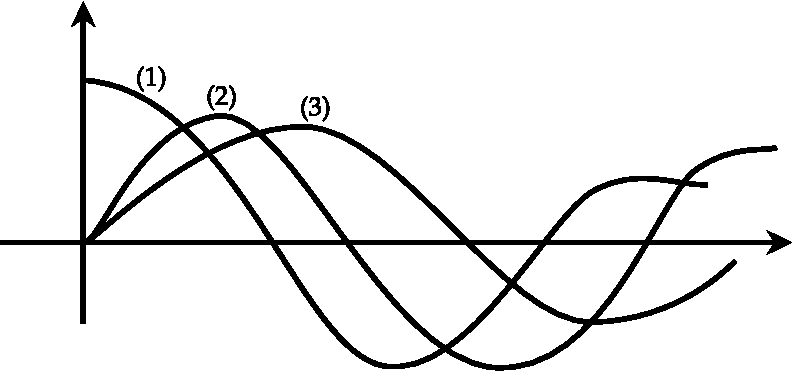
\includegraphics[height=3.5cm,width=6.5cm]{SF-01}
\end{figure}
 \begin{tasks}(2)
	\task[\textbf{a.}](1) $J_{0}$,
	(2) $J_{2}$, (3) $J_{1}$
	\task[\textbf{b.}]$(1) J_{0}$,
	(2) $J_{1}, \quad(3) J_{2}$
	\task[\textbf{c.}](1) $J_{2}$,
	(2) $J_{1}$,
	(3) $J_{0}$
	\task[\textbf{d.}] None of the above
\end{tasks}
\begin{answer}
	So the correct answer is \textbf{Option (b)}
\end{answer}
\item If the generating function of Legendre polynomial is $\frac{1}{\sqrt{1-6 t+t^{2}}}$, then coefficient of $t^{2}$ is
 \begin{tasks}(4)
	\task[\textbf{a.}] 11
	\task[\textbf{b.}]$-11$
	\task[\textbf{c.}]13
	\task[\textbf{d.}] $-13$
\end{tasks}
\begin{answer}
	\begin{align*}
	\intertext{The generating function for the polynomial solutions of the Legendre ODE is given by}
	g(x, t)&=\frac{1}{\sqrt{1-2 x t+t^{2}}}=\sum_{n=0}^{\infty} P_{n}(x) t^{n}\\
	\text{Thus }x&=3\text{ and }n=2.\\
	P_{2}(x)&=\frac{1}{2}\left(3 x^{2}-1\right) \Rightarrow P_{2}(3)=\frac{1}{2}\left(3 \times 3^{2}-1\right)=13
	\end{align*}
		So the correct answer is \textbf{Option (c)}
\end{answer}
\item Which of the following relation is true for Bessel's differential equation?
 \begin{tasks}(2)
	\task[\textbf{a.}]$J_{0}^{\prime}(x)=J_{1}(x)$
	\task[\textbf{b.}]$J_{0}^{\prime}(x)=-J_{2}(x)$
	\task[\textbf{c.}]$J_{0}^{\prime}(x)=J_{2}(x)$
	\task[\textbf{d.}] $J_{0}^{\prime}(x)=-J_{1}(x)$
\end{tasks}
\begin{answer}
	So the correct answer is \textbf{Option (d)}
\end{answer}
\item Given that $\sum_{n=0}^{\infty} H_{n}(x) \frac{t^{n}}{n !}=e^{-t^{2}+2 x x}$ the value of $H_{6}(0)$ is
 \begin{tasks}(4)
	\task[\textbf{a.}]$-120$
	\task[\textbf{b.}]$+120$
	\task[\textbf{c.}]12
	\task[\textbf{d.}]  $-12$
\end{tasks}
\begin{answer}
	\begin{align*}
	\sum_{n=0}^{\infty} I_{n}(x) \frac{t^{\prime \prime}}{n !}&=e^{-t^{2}+2 t x} \Rightarrow \sum_{n=0}^{\infty} H_{n}(0) \frac{t^{n}}{n !}=e^{-t^{2}}=1-t^{2}+\frac{t^{4}}{2 !}-\frac{t^{6}}{3 !}\\
	\Rightarrow \frac{H_{6}(0)}{6 !} t^{6}&=-\frac{1}{3 !} t^{6} \Rightarrow H_{6}(0)=-\frac{6 !}{3 !}=-120
	\end{align*}
	So the correct answer is \textbf{Option (a)}
\end{answer}
\item Given that $\sum_{n=0}^{\infty} H_{n}(x) \frac{t^{n}}{n !}=e^{-t^{2}+2 e x}$ the value of $H_{4}(0)$ is
 \begin{tasks}(4)
	\task[\textbf{a.}]12
	\task[\textbf{b.}] 6
	\task[\textbf{c.}]24
	\task[\textbf{d.}] $-6$
\end{tasks}
\begin{answer}
	\begin{align*}
	\sum_{n=0}^{\infty} H_{n}(x) \frac{t^{n}}{n !}&=e^{-t^{2}+2 t x} \Rightarrow \sum_{n=0}^{\infty} H_{n}(0) \frac{t^{n}}{n !}=e^{-t^{2}}=1-t^{2}+\frac{t^{4}}{2 !}-\frac{t^{6}}{3 !}\\
	\Rightarrow \frac{H_{4}(0)}{4 !} t^{4}&=\frac{t^{4}}{2 !} \Rightarrow H_{4}(0)=\frac{4 !}{2 !}=12
	\end{align*}
	So the correct answer is \textbf{Option (a)}
\end{answer}
\item If Hermite polynomial of order 2 is given by $H_{2}(x)=a x^{2}-2 ; a>0$, then the value of $a$ is
 \begin{tasks}(4)
	\task[\textbf{a.}]3
	\task[\textbf{b.}]4
	\task[\textbf{c.}]5
	\task[\textbf{d.}] 6
\end{tasks}
\begin{answer}
	\begin{align*}
	\intertext{Orthonormality condition,}
	\int_{-\infty}^{+\infty}\left[H_{n}(x)\right]^{2} e^{-x^{2}} d x&=2^{\prime \prime} n ! \sqrt{\pi}\\
	\text{For, }n&=2, \int_{-\infty}^{+\infty}\left(a x^{2}-2\right)^{2} e^{-x^{2}} d x=8 \sqrt{\pi}\\
\text{	Now}
	\int_{-\infty}^{+\infty}\left[H_{2}(x)\right]^{2} e^{-x^{2}} d x&=\int_{-\infty}^{+\infty}\left(a x^{2}-2\right)^{2} e^{-x^{2}} d x=\left\{a^{2} \times \frac{3}{4}+4-2 a\right\} \sqrt{\pi}
	\intertext{Thus, we have}
	\frac{3 a^{2}}{4}+4-2 a&=8 \Rightarrow 3 a^{2}-8 a-16=0 \Rightarrow 3 a^{2}-12 a+4 a-16=0\\
	\Rightarrow 3 a(a-4)+4(a-4)&=0 \Rightarrow(3 a+4)(a-4)=0\\
	\text{Thus, }a&=4
	\end{align*}
		So the correct answer is \textbf{Option (b)}
\end{answer}
\item The value of Legendre polynomial $p_{n}(x)$ for odd $n$ and $x=0$. i.e., $p_{n}(0)$ is
 \begin{tasks}(4)
	\task[\textbf{a.}]1
	\task[\textbf{b.}]0
	\task[\textbf{c.}]$-1$
	\task[\textbf{d.}]  $0.5$
\end{tasks}
\begin{answer}
	\begin{align*}
	\intertext{The generating function for Legendre polynomial is}
	\left(1-2 x t+t^{2}\right)^{-1 / 2}&=\sum_{n=0}^{\infty} p_{n}(x) t^{n}\\
	\text{Put, $x=0$, we get, }&\left(1+t^{2}\right)^{-1 / 2}=\sum p_{n}(\theta) t^{n}
	\end{align*}
		So the correct answer is \textbf{Option (b)}
\end{answer}
\item For the Legendre's polynomial $P_{n}(x)$, given below are two statements. Study these carefully and pick out the correct option.\\
Statement I: $\quad \int_{-1}^{1} x\left[P_{n}(x)\right]^{2} d x=0$\\
Statement I: $\lim _{n \rightarrow \infty}\left[\int_{-1}^{1} x P_{n}(x) P_{n+1}(x) d x\right]=0$
 \begin{tasks}(1)
	\task[\textbf{a.}]Only statement (I) is correct
	\task[\textbf{b.}]Only statement (II) is correct
	\task[\textbf{c.}]Both (I) and (II) are correct
	\task[\textbf{d.}]Neither (I) nor (II) is correet
\end{tasks}
\begin{answer}
	\begin{align*}
	\intertext{From recurrence relation we have}
	(n+1) P_{n+1}(x)&=(2 n+1) x p_{n}(x)-n p_{n-1}(x)\\
	x p_{n}(x)&=\frac{1}{(2 n+1)}\left\{(n+1) p_{n+1}(x)+n p_{n-1}(x)\right\}\\
	x\left[p_{n}(x)\right]^{2}&=\frac{1}{(2 n+1)}\left\{(n+1) p_{n}(x) p_{n+1}(x)+n p_{n}(x) p_{n-1}(x)\right\}\\
	\therefore \int_{-1}^{+1} x\left[p_{n}(x)\right]^{2} d x&=0\left\{\because \int_{-1}^{+1} p_{m}(x) p_{n}(x)=0\right.\text{ if }\left.m \neq n\right\}\\
	\therefore &\int_{-1}^{+1} x\left[p_{n}(x)\right]^{2} d x=0
	\intertext{From recurrence relation, we have}
	(n+1) p_{n+1}(x)&=(2 n+1) x p_{n}(x)-n p_{n-1}(x)\\
	(2 n+1) x p_{n}(x)&=(n+1) p_{n+1}(x)+n p_{n-1}(x)\\
	\int_{-1}^{+1}(2 n+1) x p_{n}(x) p_{n+1}(x) d x&=\int_{-1}^{+1}\left[(n+1)\left\{p_{n+1}(x)\right\}^{2}+n p_{n-1}(x) p_{n+1}(x)\right] d x\\
	=\int_{-1}^{+1}(n+1)\left\{p_{n+1}(x)\right\}^{2} d x+n \int_{-1}^{+1}& p_{n-1}(x) p_{n+1}(x) d x=(n+1) \frac{2}{2(n+1)+1}+0=\frac{2 n+2}{2 n+3}\\
	\therefore \int_{-1}^{+1} x p_{n}(x) p_{n+1}(x) d x&=\frac{2 n+2}{(2 n+1)(2 n+3)}\\
	\lim _{n \rightarrow \infty} \frac{n\left(2+\frac{2}{n}\right)}{n^{2}\left(2+\frac{1}{n}\right)\left(2+\frac{3}{n}\right)}&=\lim _{n \rightarrow \infty} \frac{\left(2+\frac{2}{n}\right)}{n\left(2+\frac{1}{n}\right)\left(2+\frac{3}{n}\right)}=0
	\end{align*}
		So the correct answer is \textbf{Option (c)}
\end{answer}
\item Which of the following statements is Incorrect about the Hermite polynomials $H_{n}(x)$ ?
 \begin{tasks}(1)
	\task[\textbf{a.}] The value of integral $\frac{1}{\sqrt{\pi}} \int_{-\infty}^{\infty} e^{-x^{2}}\left[H_{4}(x)\right]^{2} d x$ is 384
	\task[\textbf{b.}] Hermite polynomial of order $3, H_{3}(x)$, satisfies the differential equation $y^{\prime \prime}-2 x y^{\prime}+6 y=0$
	\task[\textbf{c.}] The value of $\mathrm{H}_{4}(\mathrm{l})$ is $-20$
	\task[\textbf{d.}] $H_{n}(x)=\frac{H_{n+1}(x)+2 n H_{n-1}(x)}{x}$
\end{tasks}
\begin{answer}
	\begin{align*}
	\intertext{When integrated with respect to weight function $e^{-x^{2}}$, the Hermite polynomials satisfy}
	\int_{-\infty}^{\infty} e^{-x^{2}} H_{n}(x) H_{m}(x) d x&= \begin{cases}0, & n \neq m \\ \sqrt{\pi} 2^{n} n !, & n=m\end{cases}
	\intertext{In our case $n=m=4$, hence}
	\frac{1}{\sqrt{\pi}} \int_{-\infty}^{\infty} e^{-x^{2}}\left[H_{4}(x)\right]^{2} d x&=\frac{\sqrt{\pi} 2^{4}(4 !)}{\sqrt{\pi}}=384
	\intertext{Hermite polynomial of order $n$, satisfies the differential equation}
	y^{\prime \prime}-2 x y^{\prime}+2 n y=0\\
\text{	when }n=3, y^{\prime \prime}-2 x y^{\prime}+6 y=0\\
	\text{We have }H_{4}(x)&=16 x^{4}-48 x^{2}+12\\
	\text{Therefore, }H_{4}(1)&=-48+28=-20
	\intertext{The recursion relation for Hermite polynomials is}
	H_{n+1}(x)&=2 x H_{n}(x)-2 n H_{n-1}(x) \Rightarrow H_{n}(x)=\frac{H_{n+1}(x)+2 n H_{n-1}(x)}{2 x}
	\end{align*}
		So the correct answer is \textbf{Option (d)}
\end{answer}
\item If $P_{n}(x)$ denotes the Legendre polynomials of order $n$, then which of the following statements is incorrect?
 \begin{tasks}(1)
	\task[\textbf{a.}]$P_{n}(x)=\frac{1}{2^{n} n !} \frac{d^{n}}{d x^{n}}\left[\left(x^{2}-1\right)^{n}\right]$ where $n=0,1,2 \ldots$
	\task[\textbf{b.}]The Legendre polynomials satisfy the differential equation\\$
	\left(1-x^{2}\right) \frac{d^{2} y}{d x^{2}}-2 x \frac{d y}{d x}+n(n+1) y=0
	$
	\task[\textbf{c.}] For each value of $n$ the Legendre polynomials satisfy the relation $P_{n}(1)=1$.
	\task[\textbf{d.}] The value of integral $\int_{-1}^{1}\left[P_{4}(x)\right]^{2} d x$ is $\frac{2}{7}$.
\end{tasks}
\begin{answer}
	\begin{align*}
	\intertext{Option (a) is the correct definition of Legendre polynomial. Legendre polynoimials satisfy the differential equation given in option (b). For each value of $n$ Legendre polynomials satisfy $P_{n}(1)=1$.}
	\text{Since, }\int_{-1}^{1}\left[P_{n}(x)\right]^{2} d x&=\frac{2}{2 n+1}\\
	\text{Hence, }\int_{-1}^{1}\left[P_{4}(x)\right]^{2} d x&=\frac{2}{2 \cdot 4+1}=\frac{2}{9}\\
	\text{Hence option }&(d)\text{ is incorrect.}
	\end{align*}
		So the correct answer is \textbf{Option (d)}
\end{answer}
\end{enumerate}
%\input{chapter/Practice set Solutions}
%\chapter{Practice set Solutions Differential Equations}
\begin{abox}
	Problem Set -1
\end{abox}
\begin{enumerate}[label=\color{ocre}\textbf{\arabic*.}]	
	\item Let $x_{1}(t)$ and $x_{2}(t)$ be two linearly independent solutions of the differential equation $\frac{d^{2} x}{d t^{2}}+2 \frac{d x}{d t}+f(t) x=0$ and let $w(t)=x_{1}(t) \frac{d x_{2}(t)}{d t}-x_{2}(t) \frac{d x_{1}(t)}{d t} .$ If $w(0)=1$, then $w(1)$ is given by
	{\exyear{ NET/JRF(DEC-2011)}}
			\begin{tasks}(4)
			\task[\textbf{A.}] 1
			\task[\textbf{B.}] $e^{2}$
			\task[\textbf{C.}]  $1 / e$
			\task[\textbf{D.}] $1 / e^{2}$
		\end{tasks}
			\begin{answer}
			\begin{align*}
			\intertext{$W(t)$ is Wronskian of D.E.}
			W&=e^{-\int \mathrm{Pdt}}=e^{-2 t} \Rightarrow W(1)\\&=e^{-2}\text{ since }P=2
			\end{align*}
			So the correct answer is \textbf{Option (D)}
		\end{answer}
\item Let $y(x)$ be a continuous real function in the range 0 and $2 \pi$, satisfying the inhomogeneous differential equation: $\sin x \frac{d^{2} y}{d x^{2}}+\cos x \frac{d y}{d x}=\delta\left(x-\frac{\pi}{2}\right)$ The value of $d y l d x$ at the point $x=\pi / 2$
{\exyear{NET/JRF (JUNE-2012)}}
\begin{tasks}(2)
	\task[\textbf{A.}] Is continuous
	\task[\textbf{B.}] Has a discontinuity of 3
	\task[\textbf{C.}] Has a discontinuity of $1 / 3$
	\task[\textbf{D.}] Has a discontinuity of 1
\end{tasks}
\begin{answer}
	\begin{align*}
	\text{After dividing by }\sin x, \frac{d^{2} y}{d x^{2}}+\cot x \frac{d y}{d x}&=\operatorname{cosec} x \cdot \delta\left(x-\frac{\pi}{2}\right)\\
	\text{Integrating both sides, }\frac{d y}{d x}+\int \cot x\left(\frac{d y}{d x}\right) d x&=\int \operatorname{cosec} x \delta\left(x-\frac{\pi}{2}\right) d x\\
	\frac{d y}{d x}+\cot x \cdot y-\int \operatorname{cosec}^{2} x \cdot y d x&=1\\
	\text{Using Dirac delta property: }\int f(x) \delta\left(x-x_{0}\right)&=f\left(x_{0}\right)\text{ (it lies with the limit).}\\
	\frac{d y}{d x}+y \cdot \frac{\cos x}{\sin x}-\int y \operatorname{cosec}^{2} x d x&=1,\text{ at }x=\pi ; \sin x=0 .\text{ So this is point of discontinuity.}
	\end{align*}
	So the correct answer is \textbf{Option (D)}
\end{answer}
\item The solution of the partial differential equation
$$
\frac{\partial^{2}}{\partial t^{2}} u(x, t)-\frac{\partial^{2}}{\partial x^{2}} u(x, t)=0
$$
satisfying the boundary conditions $u(0, t)=0=u(L, t)$ and initial conditions $u(x, 0)=\sin (\pi x / L)$ and $\left.\frac{\partial}{\partial t} u(x, t)\right|_{t=0}=\sin (2 \pi x / L)$ is
{\exyear{NET/JRF(JUNE-2013)}}
	\begin{tasks}(1)
		\task[\textbf{A.}] $\sin (\pi x / L) \cos (\pi t / L)+\frac{L}{2 \pi} \sin (2 \pi x / L) \cos (2 \pi t / L)$
		\task[\textbf{B.}] $2 \sin (\pi x / L) \cos (\pi t / L)-\sin (\pi x / L) \cos (2 \pi t / L)$
		\task[\textbf{C.}] $\sin (\pi x / L) \cos (2 \pi t / L)+\frac{L}{\pi} \sin (2 \pi x / L) \sin (\pi t / L)$
		\task[\textbf{D.}] $\sin (\pi x / L) \cos (\pi t / L)+\frac{L}{2 \pi} \sin (2 \pi x / L) \sin (2 \pi t / L)$
	\end{tasks}
	\begin{answer}
		\begin{align*}
		\frac{\partial^{2} u}{\partial t^{2}}-\frac{\partial^{2} u}{\partial x^{2}}&=0, u(x, 0)=\sin \frac{\pi x}{L}\text{ and }\left.\frac{\partial u}{\partial t}\right|_{t=0}=\sin \frac{2 \pi x}{L}\\
		\text{This is a wave equation}\\
		\text{So solution is given by }u(x, t)&=\sum_{n}\left(A_{n} \cos \frac{a n \pi t}{L}+B_{n} \sin \frac{a n \pi t}{L}\right) \sin \left(\frac{n \pi x}{L}\right)\\
		\text{with }A_{n}&=\frac{2}{L} \int_{0}^{L} f(x) \sin \frac{n \pi x}{L} d x, \\ B_{n}&=\frac{2}{a n \pi} \int_{0}^{L} g(x) \sin \frac{n \pi x}{L} d x\\
		\text{Comparing }a^{2} \frac{\partial^{2} u}{\partial t^{2}}&=\frac{\partial^{2} u}{\partial x^{2}},\text{ We have }a=1\text{ and }f(x)\\&=\sin \frac{\pi x}{L}, g(x)=\sin \frac{2 \pi x}{L}\\
		A_{n}&=\frac{2}{L} \int_{0}^{L} \sin \frac{\pi x}{L} \sin \frac{n \pi x}{L} d x \Rightarrow \frac{2}{L} \int_{0}^{L} \sin ^{2} \frac{\pi x}{L} d x\\&=\frac{2}{L} \int_{0}^{L}\left(\frac{1-\cos \frac{2 \pi x}{L}}{2}\right) d x=\frac{2}{L} \cdot \frac{L}{2}=1 (\text{let }\left.n=1\right)\\
		\text{Putting }n&=2, B_{n}=\frac{2}{a n \pi} \int_{0}^{L} \sin \frac{2 \pi x}{L} \cdot \sin \frac{n \pi x}{L} d x\\
		\Rightarrow \frac{2}{2 \pi} \int_{0}^{L} \sin ^{2} \frac{2 \pi x}{L} d x&=\frac{2}{2 \pi} \int_{0}^{L}\left(\frac{1-\cos \frac{4 \pi x}{L}}{2}\right) d x=\frac{2}{2 \pi} \cdot \frac{L}{2}=\frac{L}{2 \pi}
		\end{align*}
		So the correct answer is \textbf{Option (D)}
	\end{answer}
	\item The solution of the differential equation
	$$
	\frac{d x}{d t}=x^{2}
	$$
	with the initial condition $x(0)=1$ will blow up as $t$ tends to
	{\exyear{NET/JRF(JUNE-2013)}}
	\begin{tasks}(4)
		\task[\textbf{A.}] 1
		\task[\textbf{B.}] 2
		\task[\textbf{C.}] $\frac{1}{2}$
		\task[\textbf{D.}] $\infty$
	\end{tasks}
	\begin{answer}
		\begin{align*}
		\frac{d x}{d t}&=x^{2} \Rightarrow \int \frac{d x}{x^{2}}=\int d t \Rightarrow \frac{x^{-2+1}}{-2+1}\\&=t+C \Rightarrow \frac{-1}{x}=t+C\\
		\Rightarrow x(0)&=1 \Rightarrow \frac{-1}{1}=0+C \Rightarrow C=-1 \Rightarrow \frac{-1}{x}\\&=t-1 \Rightarrow x=\frac{1}{1-t}\text{ as }t \rightarrow 1, x\text{ blows up}
		\end{align*}
		So the correct answer is \textbf{Option (A)}
	\end{answer}
	\item Consider the differential equation
	$$
	\frac{d^{2} x}{d t^{2}}+2 \frac{d x}{d t}+x=0
	$$
	with the initial conditions $x(0)=0$ and $\dot{x}(0)=1$. The solution $x(t)$ attains its maximum value when $t$ is
	{\exyear{NET/JRF(JUNE-2014)}}
	\begin{tasks}(4)
		\task[\textbf{A.}] $1 / 2$
		\task[\textbf{B.}] 1
		\task[\textbf{C.}] 2
		\task[\textbf{D.}] $\infty$
	\end{tasks}
	\begin{answer}
		\begin{align*}
		\frac{d^{2} x}{d t^{2}}+2 \frac{d x}{d t}+x&=0 \Rightarrow m^{2}+2 m+1\\&=0 \Rightarrow(m+1)^{2}=0 \Rightarrow m=-1,-1\\
		\Rightarrow x&=\left(c_{1}+c_{2} t\right) e^{-t},\text{ since }x(0)\\&=0 \Rightarrow 0=c_{1} \Rightarrow x=c_{2} t e^{-t}\\
		\Rightarrow \dot{x}&=c_{2}\left[-t e^{-t}+e^{-t}\right]\\
		\text{Since }\dot{x}(0)&=1 \Rightarrow 1=c_{2} \Rightarrow x=t e^{-t}\\
		\text{For maxima or minima }\dot{x}&=0 \Rightarrow \dot{x}=-t e^{-t}+e^{-t}=0 \Rightarrow \dot{x}=e^{-t}(1-t)\\
		\Rightarrow e^{-t}&=0,1-t=0 \Rightarrow t=\infty, t=1\\
		\ddot{x}&=e^{-t}(-1)+(1-t) e^{-t}(-1)\\&=-e^{-t}+(t-1) e^{-t} \Rightarrow \ddot{x}(1)\\&=-e^{-1}+0 e^{-t}<0
		\end{align*}
		So the correct answer is \textbf{Option (B)}
	\end{answer}
	\item Consider the differential equation $\frac{d^{2} x}{d t^{2}}-3 \frac{d x}{d t}+2 x=0$. If $x=0$ at $t=0$ and $x=1$ at $t=1$, the value of $x$ at $t=2$ is
	{\exyear{NET/JRF(JUNE-2015)}}
	\begin{tasks}(4)
		\task[\textbf{A.}] $e^{2}+1$
		\task[\textbf{B.}] $e^{2}+e$
		\task[\textbf{C.}] $e+2$
		\task[\textbf{D.}] $2 e$
	\end{tasks}
	\begin{answer}
		\begin{align*}
		D^{2}-3 D+2&=0\\
		(D-1)(D-2)&=0 \Rightarrow D=1,2 \Rightarrow x=c_{1} e^{2 t}+c_{2} e^{t}\\
		\text{using boundary condition }x&=0, t=0 \Rightarrow c_{1}=-C_{2}\\
		\text{again using boundary condition }x&=1, t=1\\
		c_{2}&=\frac{1}{e-e^{2}}, c_{1}=\frac{1}{e^{2}-e} \Rightarrow x\\&=\frac{e^{2 t}}{e^{2}-e}+\frac{1}{e-e^{2}} e^{t}\\
		\text{again using }t&=2\text{ then }x=e^{2}+e
		\end{align*}
		So the correct answer is \textbf{Option (B)}
	\end{answer}
	\item  If $y=\frac{1}{\tanh (x)}$, then $x$ is
	{\exyear{NET/JRF(DEC-2015)}}
	\begin{tasks}(4)
		\task[\textbf{A.}] $\ln \left(\frac{y+1}{y-1}\right)$
		\task[\textbf{B.}] $\ln \left(\frac{y-1}{y+1}\right)$
		\task[\textbf{C.}]  $\ln \sqrt{\frac{y-1}{y+1}}$
		\task[\textbf{D.}]  $\ln \sqrt{\frac{y+1}{y-1}}$
	\end{tasks}
	\begin{answer}
		\begin{align*}
		y&=\frac{1}{\tanh x}\\
		y&=\frac{e^{x}+e^{-x}}{e^{x}-e^{-x}}=\frac{e^{2 x}+1}{e^{2 x}-1}\\
		y e^{2 x}-y&=e^{2 x}+1 \Rightarrow y e^{2 x}-e^{2 x}\\&=1+y \Rightarrow e^{2 x}(y-1)=(1+y)\\
		2 x&=\ln \left(\frac{y+1}{y-1}\right) \Rightarrow x=\frac{1}{2} \ln \left(\frac{y+1}{y-1}\right)\\&=\ln \left(\frac{y+1}{y-1}\right)^{\frac{1}{2}}
		\end{align*}
		So the correct answer is \textbf{Option (D)}
	\end{answer}
	\item The solution of the differential equation $\frac{d x}{d t}=2 \sqrt{1-x^{2}}$, with initial condition $x=0$ at $t=0$ is
	{\exyear{NET/JRF(DEC-2015)}}
	\begin{tasks}(2)
		\task[\textbf{A.}] $x=\left\{\begin{array}{ll}\sin 2 t, & 0 \leq t<\frac{\pi}{4} \\ \sinh 2 t, & t \geq \frac{\pi}{4}\end{array}\right.$
		\task[\textbf{B.}] $x=\left\{\begin{array}{cc}\sin 2 t, & 0 \leq t<\frac{\pi}{2} \\ 1, & t \geq \frac{\pi}{2}\end{array}\right.$
		\task[\textbf{C.}] $x=\left\{\begin{array}{cc}\sin 2 t, & 0 \leq t<\frac{\pi}{4} \\ 1, & t \geq \frac{\pi}{4}\end{array}\right.$
		\task[\textbf{D.}] $x=1-\cos 2 t, \quad t \geq 0$
	\end{tasks}
	\begin{answer}
		\begin{align*}
		\frac{d x}{d t}&=2 \sqrt{1-x^{2}}, \frac{d x}{\sqrt{1-x^{2}}}\\&=2 d t, \sin ^{-1} x=2 t+c, x=0, t=0 \\\text{ so, }c&=0 \Rightarrow x=\sin 2 t\\
		&\text{	$x$ should not be greater than 1 at $x=1$}\\
		1&=\sin 2 t, \quad \sin \frac{\pi}{2}=\sin 2 t, t=\frac{\pi}{4}\\
		\text{	So, }\quad x&=\left\{\begin{array}{ll}\sin 2 t, & 0 \leq t<\frac{\pi}{4} \\ 1, & t \geq \frac{\pi}{4}\end{array}\right.
		\end{align*}
		So the correct answer is \textbf{Option (C)}
	\end{answer}
	\item   The function $y(x)$ satisfies the differential equation $x \frac{d y}{d x}+2 y=\frac{\cos \pi x}{x}$. If $y(1)=1$, the value of $y(2)$ is
	{\exyear{NET/JRF(JUNE-2017)}}
	\begin{tasks}(4)
		\task[\textbf{A.}] $\pi$
		\task[\textbf{B.}] 1
		\task[\textbf{C.}] $1 / 2$
		\task[\textbf{D.}] $1 / 4$
	\end{tasks}
	\begin{answer}
		\begin{align*}
		\intertext{The given differential equation can be written as}
		\frac{d y}{d x}+\frac{2}{x} y&=\frac{\cos \pi x}{x^{2}}
		\intertext{This is a linear differential equation with Integrating factor $=e^{\int_{x}^{2} d x}=x^{2}$}
		\text{Hence }y . x^{2}&=\int x^{2} \cdot \frac{\cos \pi x}{x^{2}} d x+c \Rightarrow y\\&=\frac{\sin \pi x}{\pi x^{2}}+\frac{c}{x^{2}}\\
		\text{when }x&=1, y=1\text{ hence }c=1 \Rightarrow y\\&=\frac{\sin \pi x}{\pi x^{2}}+\frac{1}{x^{2}}\\
		\text{hence, when }x&=2, y=\frac{1}{4}
		\end{align*}
		So the correct answer is \textbf{Option (D)}
	\end{answer}
	\item   Consider the differential equation $\frac{d y}{d t}+a y=e^{-b t}$ with the initial condition $y(0)=0$. Then the Laplace transform $Y(s)$ of the solution $y(t)$ is
	{\exyear{NET/JRF(DEC-2017)}}
	\begin{tasks}(4)
		\task[\textbf{A.}] $\frac{1}{(s+a)(s+b)}$
		\task[\textbf{B.}] $\frac{1}{b(s+a)}$
		\task[\textbf{C.}] $\frac{1}{a(s+b)}$
		\task[\textbf{D.}] $\frac{e^{-a}-e^{-b}}{b-a}$
	\end{tasks}
	\begin{answer}
		\begin{align*}
		\text{Given }\frac{d y}{d t}+a y&=e^{-b t}
		\intertext{Taking Laplace transform of both sides}
		\text{	We obtain}\\
		L\left\{\frac{d y}{d t}\right\}+a L\{y(t)\}&=L\left\{e^{-b t}\right\} \Rightarrow s Y(s)-y(0)+a Y(s)=\frac{1}{s+b}\\
		\text{Since, }	y(0)&=0,\text{ we obtain}\\
		(s+a) Y(s)&=\frac{1}{s+b} \Rightarrow Y(s)=\frac{1}{(s+a)(s+b)}
		\end{align*}
		So the correct answer is \textbf{Option (A)}
	\end{answer}
	\item The number of linearly independent power series solutions, around $x=0$, of the second order linear differential equation $x \frac{d^{2} y}{d x^{2}}+\frac{d y}{d x}+x y=0$, is
	{\exyear{NET/JRF(DEC-2017)}}
	\begin{tasks}(1)
		\task[\textbf{A.}] 0 (this equation does not have a power series solution)
		\task[\textbf{B.}] 1
		\task[\textbf{C.}] 2
		\task[\textbf{D.}] 3
	\end{tasks}
	\begin{answer}
		So the correct answer is \textbf{Option (B)}
	\end{answer}
	\item The differential equation $\frac{d y(x)}{d x}=\alpha x^{2}$, with the initial condition $y(0)=0$, is solved using Euler's method. If $y_{E}(x)$ is the exact solution and $y_{N}(x)$ the numerical solution obtained using $n$ steps of equal length, then the relative error $\left|\frac{\left(y_{N}(x)-y_{E}(x)\right)}{y_{E}(x)}\right|$ is proportional to
	{\exyear{NET/JRF(DEC-2017)}}
	\begin{tasks}(4)
		\task[\textbf{A.}] $\frac{1}{n^{2}}$
		\task[\textbf{B.}] $\frac{1}{n^{3}}$
		\task[\textbf{C.}] $\frac{1}{n^{4}}$
		\task[\textbf{D.}] $\frac{1}{n}$
	\end{tasks}
	\begin{answer}
		\begin{align*}
		\frac{d y}{d x}&=\alpha x^{2}, y(0)=0\\
		y_{E}&=\frac{\alpha x^{3}}{3},\text{ but }x=n \hbar\\
		\text{Exact solution, }y_{E}&=\frac{\alpha n^{3} h^{3}}{3}\\
		\text{Numerically, }f(x, y)&=\alpha x^{2}\\
		\text{Euler's method, }y_{i}&=y_{i-1}+h f\left(x_{i-1}, y_{i-1}\right)\\
		y_{1}&=0, y_{2}=\alpha h^{3} \quad y_{3}=5 \alpha h^{3}\\
		y_{n}&=\frac{(n-1) n(2 n-1)}{6} \alpha h^{3}
		\intertext{Since, $0,5,14,30, \ldots$ different from square terms}
		\intertext{At, $x_{0}=0 \quad x_{1}=x_{0}+h=h \quad x_{2}=x_{0}+2 h=2 h \quad x_{3}=x_{0}+3 h=3 h$}
		x_{n-1}&=x_{0}+(n-1) h=(n-1) h .\text{ Now, }x_{n}=n h\\
		f\left(x_{0}, y_{0}\right)
		&=0, f\left(x_{1}, y_{1}\right)=\alpha h^{2}, f\left(x_{2}, y_{2}\right)=4 \alpha h^{2}\\
		f\left(x_{n-1}, y_{n-1}\right)&=\alpha(n-1)^{2} h^{2}\\
		\left|\frac{\left(y_{N}-y_{E}\right)}{y_{E}}\right|&=\left|\frac{\frac{(n-1) n(2 n-1) \alpha h^{3}}{6}-\frac{\alpha n^{3} h^{3}}{3}}{\frac{\alpha n^{3} h^{3}}{3}}\right|\\
		\text{By solving, }&\left|\frac{y_{N}-y_{E}}{y_{E}}\right| \propto \frac{1}{n}
		\end{align*}
		So the correct answer is \textbf{Option (D)}
	\end{answer}
	\item  Consider the following ordinary differential equation
	$$
	\frac{d^{2} x}{d t^{2}}+\frac{1}{x}\left(\frac{d x}{d t}\right)^{2}-\frac{d x}{d t}=0
	$$
	with the boundary conditions $x(t=0)=0$ and $x(t=1)=1 .$ The value of $x(t)$ at $t=2$ is
	{\exyear{NET/JRF(JUNE-2018)}}
	\begin{tasks}(4)
		\task[\textbf{A.}] $\sqrt{e-1}$
		\task[\textbf{B.}] $\sqrt{e^{2}+1}$
		\task[\textbf{C.}]  $\sqrt{e+1}$
		\task[\textbf{D.}] $\sqrt{e^{2}-1}$
	\end{tasks}
	\begin{answer}
		\begin{align*}
		\intertext{The given equation can be written as}
		\frac{1}{x} \frac{d}{d t}\left(x \frac{d x}{d t}\right)-\frac{d x}{d t}&=0 \Rightarrow \frac{d}{d t}\left(x \frac{d x}{d t}\right)-x \frac{d x}{d t}=0\\
		\text{putting }y&=x \frac{d x}{d t}\text{ gives}\\
		\frac{d y}{d t}-y&=0 \Rightarrow \ln y=t+\ln c_{1} \Rightarrow y=c_{1} e^{t}\\
		\intertext{Since $x \frac{d x}{d t}=c_{1} e^{t}$ hence by integrating}
		\frac{x^{2}}{2}&=c_{1} e^{t}+c_{2}\hspace{2cm}\text{(i)}
		\intertext{Using boundary conditions we obtain}
		c_{1}+c_{2}&=0\text{ and }c_{1} e+c_{2}=\frac{1}{2}
		\intertext{Solving these equations we obtain $c_{1}=\frac{1}{2(e-1)}$ and $c_{2}=-\frac{1}{2(e-1)}$}
		\text{Thus, }\frac{x^{2}}{2}&=\frac{1}{2(e-1)} e^{t}-\frac{1}{2(e-1)}\\
		\text{When }t&=2,\text{ we obtain, }\quad x^{2}=\frac{e^{2}}{(e-1)}-\frac{1}{(e-1)}\\&=\frac{\left(e^{2}-1\right)}{(e-1)}=e+1\\
		\text{Therefore}x(2)&=\sqrt{e+1}
		\end{align*}
		So the correct answer is \textbf{Option (C)}
	\end{answer}
	\item  In terms of arbitrary constants $A$ and $B$, the general solution to the differential equation $x^{2} \frac{d^{2} y}{d x^{2}}+5 x \frac{d y}{d x}+3 y=0$ is
	{\exyear{NET/JRF(DEC-2018)}}
	\begin{tasks}(4)
		\task[\textbf{A.}]  $y=\frac{A}{x}+B x^{3}$
		\task[\textbf{B.}] $y=A x+\frac{B}{x^{3}}$
		\task[\textbf{C.}] $y=A x+B x^{3}$
		\task[\textbf{D.}] $y=\frac{A}{x}+\frac{B}{x^{3}}$
	\end{tasks}
	\begin{answer}
		\begin{align*}
		\intertext{
			The given equation is Euler-Cauchy differential equation. The characteristic equation of}
		x^{2} \frac{d^{2} y}{d x^{2}}+5 x \frac{d y}{d x}+6 y&=0\\
		\text{is ,}m^{2}+4 m+6&=0 \Rightarrow m=-3 or m=-1\\
		\text{Thus, }y_{1}&=x^{-1}=\frac{1}{x}\text{ and }y_{2}=x^{2}=\frac{1}{x^{3}}
		\intertext{Therefore the general solution is}
		y&=\frac{A}{x}+\frac{B}{x^{3}}
		\end{align*}
		So the correct answer is \textbf{Option (D)}
	\end{answer}
	\item The solution of the differential equation $x \frac{d y}{d x}+(1+x) y=e^{-x}$ with the boundary condition $y(x=1)=0$, is
	{\exyear{NET/JRF(JUNE-2019)}}
	\begin{tasks}(4)
		\task[\textbf{A.}] $\frac{(x-1)}{x} e^{-x}$
		\task[\textbf{B.}] $\frac{(x-1)}{x^{2}} e^{-x}$
		\task[\textbf{C.}] $\frac{(1-x)}{x^{2}} e^{-x}$
		\task[\textbf{D.}] $(x-1)^{2} e^{-x}$
	\end{tasks}
	\begin{answer}
		\begin{align*}
		x \frac{d y}{d x}+(1+x) y&=e^{-x} \Rightarrow \frac{d y}{d x}+\frac{(1+x)}{x} y=\frac{e^{-x}}{x}\\
		\text{Let }p&=\frac{1+x}{x}\\
		I.F &=e^{\int p d x}=e^{\int\left(1+\frac{1}{x}\right) d x}=e^{x} \cdot e^{\ln x}=x e^{x}\\
		y \cdot x \cdot e^{x}&=\int \frac{e^{-x}}{x} \cdot x e^{x} d x+C \Rightarrow y \cdot x \cdot e^{x}=x+C\\
		y&=0\text{ at }x=1 \quad \Rightarrow C=-1 \quad \Rightarrow y \cdot x \cdot e^{x}\\&=x-1 \Rightarrow y=\left[\frac{x-1}{x}\right] e^{-x}
		\end{align*}
		So the correct answer is \textbf{Option (A)}
	\end{answer}
	\item The solution of the differential equation $\left(\frac{d y}{d x}\right)^{2}-\frac{d^{2} y}{d x^{2}}=e^{y}$, with the boundary conditions $y(0)=0$ and $y^{\prime}(0)=-1$, is
	{\exyear{NET/JRF(JUNE-2020)}}
	\begin{tasks}(4)
		\task[\textbf{A.}] $-\ln \left(\frac{x^{2}}{2}+x+1\right)$
		\task[\textbf{B.}] $-x \ln (e+x)$
		\task[\textbf{C.}] $-x e^{-x^{2}}$
		\task[\textbf{D.}]  $-x(x+1) e^{-x}$
	\end{tasks}
	\begin{answer}
		\begin{align*}
		\left(\frac{d y}{d x}\right)^{2}-\frac{d^{2} y}{d x^{2}}&=e^{y}\text{ put }y=\ln p\\
		\frac{d y}{d x}&=\frac{1}{p} \frac{d p}{d x} \Rightarrow \frac{d^{2} y}{d x^{2}}=\frac{d}{d x}\left(\frac{1}{p} \frac{d p}{d x}\right)\\&=\frac{1}{p} \frac{d^{2} p}{d x^{2}}-\frac{1}{p^{2}}\left(\frac{d p}{d x}\right)^{2}\\
		\text{Thus }&\left(\frac{1}{p} \frac{d p}{d x}\right)^{2}-\frac{1}{p} \frac{d^{2} p}{d x^{2}}+\frac{1}{p^{2}}\left(\frac{d p}{d x}\right)^{2}=p\\
		\frac{2}{p^{2}}\left(\frac{d p}{d x}\right)^{2}-\frac{1}{p} \frac{d^{2} p}{d x^{2}}&=p \Rightarrow \frac{2}{p^{3}}\left(\frac{d p}{d x}\right)^{2}-\frac{1}{p^{2}} \frac{d^{2} p}{d x^{2}}\\&=1 \Rightarrow \frac{1}{p^{2}} \frac{d^{2} p}{d x^{2}}-\frac{2}{p^{3}}\left(\frac{d p}{d x}\right)^{2}=-1\\
		&\Rightarrow \frac{d}{d x}\left(\frac{1}{p^{2}} \frac{d p}{d x}\right)=-1\\
		\text{Let }\frac{1}{p^{2}} \frac{d p}{d x}&=z \Rightarrow \frac{d z}{d x}=-1 \Rightarrow z=-x+c\\
		\text{Thus }\frac{1}{p^{2}} \frac{d p}{d x}&=-x+c \Rightarrow \int \frac{d p}{p^{2}}=\int(-x+c) d x\\
		-\frac{1}{p}&=-\frac{x^{2}}{2}+c x+d \Rightarrow p=\frac{1}{\frac{x^{2}}{2}-c x-d}\\
		y&=\ln p=\ln \left(\frac{1}{\frac{x^{2}}{2}-c x-d}\right)=\ln \left(\frac{x^{2}}{2}-c x-d\right)\\
		y(0)&=0 \Rightarrow y(0)=-\ln (-d) \Rightarrow d=-1\\
		y&=-\ln \left(\frac{x^{2}}{2}-c x+1\right)\\
		y^{\prime}(x)&=-\frac{1}{\left(\frac{x^{2}}{2}-c x+1\right)}(x-c), \quad y^{\prime}(0)\\&=-1 \Rightarrow-\frac{(-c)}{1}=c=-1, \quad y=-\ln \left(\frac{x^{2}}{2}+x+1\right)
		\end{align*}
		So the correct answer is \textbf{Option (A)}
	\end{answer}
\end{enumerate}
 \colorlet{ocre1}{ocre!70!}
\colorlet{ocrel}{ocre!30!}
\setlength\arrayrulewidth{1pt}
\begin{table}[H]
	\centering
	\arrayrulecolor{ocre}
	\begin{tabular}{|p{1.5cm}|p{1.5cm}||p{1.5cm}|p{1.5cm}|}
		\hline
		\multicolumn{4}{|c|}{\textbf{Answer key}}\\\hline\hline
		\rowcolor{ocrel}Q.No.&Answer&Q.No.&Answer\\\hline
		1&\textbf{D} &2&\textbf{D}\\\hline 
		3&\textbf{D} &4&\textbf{A} \\\hline
		5&\textbf{B} &6&\textbf{B} \\\hline
		7&\textbf{D}&8&\textbf{C}\\\hline
		9&\textbf{D}&10&\textbf{A}\\\hline
		11&\textbf{B} &12&\textbf{D}\\\hline
		13&\textbf{C}&14&\textbf{D}\\\hline
		15&\textbf{A}&16&\textbf{A} \\\hline
		
	\end{tabular}
\end{table}
\newpage
\begin{abox}
	Problem Set -2
\end{abox}
\begin{enumerate}[label=\color{ocre}\textbf{\arabic*.}]
	\item  The solution of the differential equation for $y(t): \frac{d^{2} y}{d t^{2}}-y=2 \cosh (t)$, subject to the initial conditions $y(0)=0$ and $\left.\frac{d y}{d t}\right|_{t=0}=0$, is
	{\exyear{GATE 2010}}
	\begin{tasks}(2)
		\task[\textbf{A.}] $\frac{1}{2} \cosh (t)+t \sinh (t)$
		\task[\textbf{B.}] $-\sinh (t)+t \cosh (t)$
		\task[\textbf{C.}] $t \cosh (t)$
		\task[\textbf{D.}] $t \sinh (t)$
	\end{tasks}
	\begin{answer}
		\begin{align}
		\text{	For C.F } \left(D^{2}-1\right) y&=0 \Rightarrow m=\pm 1 \Rightarrow C . F .\notag\\&=C_{1} e^{t}+C_{2} e^{-t}\notag\\
		P.I. &=\frac{1}{D^{2}-1}(2 \cosh t)=\frac{1}{D^{2}-1} 2\left(\frac{e^{t}+e^{-t}}{2}\right)\notag\\&=\frac{1}{D^{2}-1}\left(e^{t}\right)+\frac{1}{D^{2}-1}\left(e^{-t}\right)\notag\\&=\frac{t}{2} e^{t}+\frac{t}{2}\left(-e^{-t}\right)\notag\\
		\Rightarrow y&=C_{1} e^{t}+C_{2} e^{-t}+\frac{t}{2} e^{t}-\frac{t}{2} e^{-t}\notag\\
		\text{As, }y(0)&=0 \Rightarrow C_{1}+C_{2}=0\label{math01}\\
		\frac{d y}{d t}&=C_{1} e^{t}-C_{2} e^{-t}+\frac{t}{2} e^{t}+\frac{1}{2} e^{t}+\frac{t}{2} e^{-t}-\frac{1}{2} e^{-t}\notag\\
		\text{Also, }\left.\frac{d y}{d t}\right|_{t=0}&=0 \Rightarrow C_{1}-C_{2}+0+\frac{1}{2}+0-\frac{1}{2}=0 \Rightarrow C_{1}-C_{2}=0\label{math02}\\
		\text{From equation (\ref{math01}) and (\ref{math02}),}\notag\\
		C_{1}&=0, C_{2}=0\notag\\
		\text{Thus }y&=\frac{t}{2} e^{t}-\frac{t}{2} e^{-t} \Rightarrow y=t \sinh t\notag
		\end{align}
		So the correct answer is \textbf{Option (D)}
	\end{answer}
	\item The solutions to the differential equation $\frac{d y}{d x}=-\frac{x}{y+1}$ are a family of
	{\exyear{GATE 2011}}
	\begin{tasks}(1)
		\task[\textbf{A.}] Circles with different radii
		\task[\textbf{B.}] Circles with different centres
		\task[\textbf{C.}]  Straight lines with different slopes
		\task[\textbf{D.}]  Straight lines with different intercepts on the $y$-axis
	\end{tasks}
	\begin{answer}
		\begin{align*}
		\frac{d y}{d x}&=-\frac{x}{y+1} \Rightarrow x d x+y d y+d y\\&=0 \Rightarrow \frac{x^{2}}{2}+\frac{y^{2}}{2}+y\\&=C_{1} \Rightarrow x^{2}+y^{2}+2 y\\&=2 C_{1}
		\Rightarrow(x-0)^{2}+(y+1)^{2}\\&=2 C_{1}+1=C
		\intertext{which is a family of circles with different radii.}
		\end{align*}
		So the correct answer is \textbf{Option (A)}
	\end{answer}
	\item The solution of the differential equation $\frac{d^{2} y}{d t^{2}}-y=0$, subject to the boundary conditions $y(0)=1$ and $y(\infty)=0$ is
	{\exyear{GATE 2014}}
	\begin{tasks}(4)
		\task[\textbf{A.}] $\cos t+\sin t$
		\task[\textbf{B.}] $\cosh t+\sinh t$
		\task[\textbf{C.}] $\cos t-\sin t$
		\task[\textbf{D.}]  $\cosh t-\sinh t$
	\end{tasks}
	\begin{answer}
		\begin{align*}
		D^{2}-1&=0 \Rightarrow D=\pm 1 \Rightarrow y(t)\\&=c_{1} e^{t}+c_{2} e^{-t}
		\intertext{Applying boundary condition,}
		y(0)&=1 \Rightarrow 1=c_{1}+c_{2}\text{ and }y(\infty)\\&=0 \Rightarrow 0=c_{1} e^{\infty}+c_{2} e^{-\infty} \Rightarrow c_{1}\\&=0, c_{2}=1\\
		\Rightarrow y(t)&=e^{-t} \Rightarrow y(t)=\cosh t-\sinh \ t
		\end{align*}
		So the correct answer is \textbf{Option (D)}
	\end{answer}
	\item  A function $y(z)$ satisfies the ordinary differential equation $y^{\prime \prime}+\frac{1}{z} y^{\prime}-\frac{m^{2}}{z^{2}} y=0$, where\\
	$m=0,1,2,3, \ldots . .$ Consider the four statements P, Q, R, S as given below.\\
	$\mathrm{P}: z^{m}$ and $z^{-m}$ are linearly independent solutions for all values of $m$\\
	Q: $z^{m}$ and $z^{-m}$ are linearly independent solutions for all values of $m>0$\\
	$\mathrm{R}$ : $\ln z$ and 1 are linearly independent solutions for $m=0$\\
	S: $z^{m}$ and $\ln z$ are linearly independent solutions for all values of $m$\\
	The correct option for the combination of valid statements is
	{\exyear{GATE 2015}}
	\begin{tasks}(4)
		\task[\textbf{A.}] P, R and S only
		\task[\textbf{B.}]  P and R only
		\task[\textbf{C.}] $\mathrm{Q}$ and $\mathrm{R}$ only
		\task[\textbf{D.}] $\mathrm{R}$ and $\mathrm{S}$ only
	\end{tasks}
	\begin{answer}
		\begin{align*}
		y^{\prime \prime}+\frac{1}{z} y^{\prime}-\frac{m^{2}}{z^{2}} y&=0 \Rightarrow z^{2} y^{\prime \prime}+z y^{\prime}-m^{2} y\\&=0, m=0,1,2,3, \ldots, \quad z=e^{x}, D=\frac{d}{d x}\\
		\text{	If }m&=0 ; \quad z^{2} y^{\prime \prime}+z y^{\prime}=0,[D(D-1)+D] y\\&=0 \Rightarrow\left[D^{2}-D+D\right] y=0\\
		D^{2} y&=0 \Rightarrow y=c_{1}+c_{2} x \Rightarrow y\\&=c_{1}+c_{2} \ln z \quad \text{( $R$ is correct)}\\
		\text{And if }m &\neq 0, m>0,\text{ then }m \neq 0,\text{ then }\left(D^{2}-m^{2}\right) y\\&=0 \Rightarrow D=\pm m\\
		y&=c_{1} e^{m x}+c_{2} e^{-m x}=c_{1} e^{m \log z}+c_{2} e^{-m \log z}\\&=c_{1} z^{m}+c_{2} z^{-m}\\
		\text{or if }m &\neq 0, m>0,\text{ then}\\
		y&=c_{1} \cosh (m \log (z))+i c_{2} \sinh (m \log (x)), \quad m>0
		\end{align*}
		So the correct answer is \textbf{Option (C)} 
	\end{answer}
	\item Consider the linear differential equation $\frac{d y}{d x}=x y$. If $y=2$ at $x=0$, then the value of $y$ at $x=2$ is given by
	{\exyear{GATE 2016}}
	\begin{tasks}(4)
		\task[\textbf{A.}]  $e^{-2}$
		\task[\textbf{B.}] $2 e^{-2}$
		\task[\textbf{C.}] $e^{2}$
		\task[\textbf{D.}]  $2 e^{2}$
	\end{tasks}
	\begin{answer}
		\begin{align*}
		\frac{d y}{d x}&=x y \Rightarrow \frac{1}{y} d y=x d x \Rightarrow \ln y\\&=\frac{x^{2}}{2}+\ln c \Rightarrow y=c e^{x^{2} / 2}\\
		\text{If }y&=2\text{ at }x=0 \Rightarrow c=2 \Rightarrow y=2 e^{x^{2} / 2}\\
		\text{	The value of $y$ at }x&=2\text{ is given by }y=2 e^{2}
		\end{align*}
		So the correct answer is \textbf{Option (D)}
	\end{answer}
	\item Consider the differential equation $\frac{d y}{d x}+y \tan (x)=\cos (x)$. If $y(0)=0, y\left(\frac{\pi}{3}\right)$ is ............... (up to two decimal places)
	{\exyear{GATE 2017}}
	\begin{answer}
		\begin{align*}
		\intertext{The given differential equation is a linear differential equation of the form}
		\frac{d y}{d x}+p(x) y&=\cos x\\
		\text{	Integrating factor }&=e^{\int p(x) d x}\\
		\text{Thus integrating factor }&=e^{\int \tan x d x}\\
		\Rightarrow I \cdot F&=e^{\ln \sec x}=\sec x
		\intertext{Thus the general solution of the given differential equation is}
		y \cdot \sec x&=\int \sec x \cdot \cos x d x+c\\
		\Rightarrow y \sec x&=x+c\\
		\text{It is given that }y(0)&=0 \Rightarrow 0 \cdot \sec 0=0+c \Rightarrow c=0
		\intertext{Thus the solution satisfying the given condition is}
		y \sec x&=x \Rightarrow y=\frac{x}{\sec x}\\
		\text{Thus the value of }&y\left(\frac{\pi}{3}\right)\text{ is}\\
		y&=\frac{\pi / 3}{\sec \pi / 3}=\frac{\pi / 3}{2}=\frac{\pi}{6}=0 \cdot 52
		\end{align*}
	\end{answer}
	\item Given
	$$
	\frac{d^{2} f(x)}{d x^{2}}-2 \frac{d f(x)}{d x}+f(x)=0
	$$
	and boundary conditions $f(0)=1$ and $f(1)=0$, the value of $f(0.5)$ is --------(up
	to two decimal places).
	{\exyear{GATE 2018}}
	\begin{answer}
		\begin{align}
		\frac{d^{2} f(x)}{d x^{2}}-2 \frac{d f(x)}{d x}+f(x)&=0\notag\\
		\text{Auxiliary equation is,}\notag\\
		\left(m^{2}-2 m+1\right)&=0 \Rightarrow(m-1)^{2}\notag\\&=0 \Rightarrow m=1,1\notag\\
		\text{Hence, the solution is}\notag\\
		f(x)&=\left(c_{1}+c_{2} x\right) e^{x}\notag\\
		\text{using boundary condition,}\notag\\
		f(0)&=c_{1} e^{0} \Rightarrow c_{1}=1 \label{ma 03}\\
		f(1)&=\left(c_{1}+c_{2}\right) e=0 \label{ma 04}\\
		\text{	From (\ref{ma 03}) and (\ref{ma 04}), }c_{2}&=-1 \label{ma 05}\notag\\
		\text{Hence, }f(x)&=(1-x) e^{x} \Rightarrow f(0.5)\notag\\&=(1-0.5) e^{0.5}=0.81\notag
		\end{align}
	\end{answer}
	\item  For the differential equation $\frac{d^{2} y}{d x^{2}}-n(n+1) \frac{y}{x^{2}}=0$, where $n$ is a constant, the product of
	its two independent solutions is
	{\exyear{GATE 2019}}
	\begin{tasks}(4)
		\task[\textbf{A.}] $\frac{1}{x}$
		\task[\textbf{B.}] $x$
		\task[\textbf{C.}] $x^{n}$
		\task[\textbf{D.}] $\frac{1}{x^{n+1}}$
	\end{tasks}
	\begin{answer}
		So the correct answer is \textbf{Option (B)}
	\end{answer}
\end{enumerate}
%\chapter{Practice set Solutions Differential Equations}
\begin{abox}
	Problem Set -1
\end{abox}
\begin{enumerate}[label=\color{ocre}\textbf{\arabic*.}]	
	\item Let $x_{1}(t)$ and $x_{2}(t)$ be two linearly independent solutions of the differential equation $\frac{d^{2} x}{d t^{2}}+2 \frac{d x}{d t}+f(t) x=0$ and let $w(t)=x_{1}(t) \frac{d x_{2}(t)}{d t}-x_{2}(t) \frac{d x_{1}(t)}{d t} .$ If $w(0)=1$, then $w(1)$ is given by
	{\exyear{ NET/JRF(DEC-2011)}}
			\begin{tasks}(4)
			\task[\textbf{A.}] 1
			\task[\textbf{B.}] $e^{2}$
			\task[\textbf{C.}]  $1 / e$
			\task[\textbf{D.}] $1 / e^{2}$
		\end{tasks}
			\begin{answer}
			\begin{align*}
			\intertext{$W(t)$ is Wronskian of D.E.}
			W&=e^{-\int \mathrm{Pdt}}=e^{-2 t} \Rightarrow W(1)\\&=e^{-2}\text{ since }P=2
			\end{align*}
			So the correct answer is \textbf{Option (D)}
		\end{answer}
\item Let $y(x)$ be a continuous real function in the range 0 and $2 \pi$, satisfying the inhomogeneous differential equation: $\sin x \frac{d^{2} y}{d x^{2}}+\cos x \frac{d y}{d x}=\delta\left(x-\frac{\pi}{2}\right)$ The value of $d y l d x$ at the point $x=\pi / 2$
{\exyear{NET/JRF (JUNE-2012)}}
\begin{tasks}(2)
	\task[\textbf{A.}] Is continuous
	\task[\textbf{B.}] Has a discontinuity of 3
	\task[\textbf{C.}] Has a discontinuity of $1 / 3$
	\task[\textbf{D.}] Has a discontinuity of 1
\end{tasks}
\begin{answer}
	\begin{align*}
	\text{After dividing by }\sin x, \frac{d^{2} y}{d x^{2}}+\cot x \frac{d y}{d x}&=\operatorname{cosec} x \cdot \delta\left(x-\frac{\pi}{2}\right)\\
	\text{Integrating both sides, }\frac{d y}{d x}+\int \cot x\left(\frac{d y}{d x}\right) d x&=\int \operatorname{cosec} x \delta\left(x-\frac{\pi}{2}\right) d x\\
	\frac{d y}{d x}+\cot x \cdot y-\int \operatorname{cosec}^{2} x \cdot y d x&=1\\
	\text{Using Dirac delta property: }\int f(x) \delta\left(x-x_{0}\right)&=f\left(x_{0}\right)\text{ (it lies with the limit).}\\
	\frac{d y}{d x}+y \cdot \frac{\cos x}{\sin x}-\int y \operatorname{cosec}^{2} x d x&=1,\text{ at }x=\pi ; \sin x=0 .\text{ So this is point of discontinuity.}
	\end{align*}
	So the correct answer is \textbf{Option (D)}
\end{answer}
\item The solution of the partial differential equation
$$
\frac{\partial^{2}}{\partial t^{2}} u(x, t)-\frac{\partial^{2}}{\partial x^{2}} u(x, t)=0
$$
satisfying the boundary conditions $u(0, t)=0=u(L, t)$ and initial conditions $u(x, 0)=\sin (\pi x / L)$ and $\left.\frac{\partial}{\partial t} u(x, t)\right|_{t=0}=\sin (2 \pi x / L)$ is
{\exyear{NET/JRF(JUNE-2013)}}
	\begin{tasks}(1)
		\task[\textbf{A.}] $\sin (\pi x / L) \cos (\pi t / L)+\frac{L}{2 \pi} \sin (2 \pi x / L) \cos (2 \pi t / L)$
		\task[\textbf{B.}] $2 \sin (\pi x / L) \cos (\pi t / L)-\sin (\pi x / L) \cos (2 \pi t / L)$
		\task[\textbf{C.}] $\sin (\pi x / L) \cos (2 \pi t / L)+\frac{L}{\pi} \sin (2 \pi x / L) \sin (\pi t / L)$
		\task[\textbf{D.}] $\sin (\pi x / L) \cos (\pi t / L)+\frac{L}{2 \pi} \sin (2 \pi x / L) \sin (2 \pi t / L)$
	\end{tasks}
	\begin{answer}
		\begin{align*}
		\frac{\partial^{2} u}{\partial t^{2}}-\frac{\partial^{2} u}{\partial x^{2}}&=0, u(x, 0)=\sin \frac{\pi x}{L}\text{ and }\left.\frac{\partial u}{\partial t}\right|_{t=0}=\sin \frac{2 \pi x}{L}\\
		\text{This is a wave equation}\\
		\text{So solution is given by }u(x, t)&=\sum_{n}\left(A_{n} \cos \frac{a n \pi t}{L}+B_{n} \sin \frac{a n \pi t}{L}\right) \sin \left(\frac{n \pi x}{L}\right)\\
		\text{with }A_{n}&=\frac{2}{L} \int_{0}^{L} f(x) \sin \frac{n \pi x}{L} d x, \\ B_{n}&=\frac{2}{a n \pi} \int_{0}^{L} g(x) \sin \frac{n \pi x}{L} d x\\
		\text{Comparing }a^{2} \frac{\partial^{2} u}{\partial t^{2}}&=\frac{\partial^{2} u}{\partial x^{2}},\text{ We have }a=1\text{ and }f(x)\\&=\sin \frac{\pi x}{L}, g(x)=\sin \frac{2 \pi x}{L}\\
		A_{n}&=\frac{2}{L} \int_{0}^{L} \sin \frac{\pi x}{L} \sin \frac{n \pi x}{L} d x \Rightarrow \frac{2}{L} \int_{0}^{L} \sin ^{2} \frac{\pi x}{L} d x\\&=\frac{2}{L} \int_{0}^{L}\left(\frac{1-\cos \frac{2 \pi x}{L}}{2}\right) d x=\frac{2}{L} \cdot \frac{L}{2}=1 (\text{let }\left.n=1\right)\\
		\text{Putting }n&=2, B_{n}=\frac{2}{a n \pi} \int_{0}^{L} \sin \frac{2 \pi x}{L} \cdot \sin \frac{n \pi x}{L} d x\\
		\Rightarrow \frac{2}{2 \pi} \int_{0}^{L} \sin ^{2} \frac{2 \pi x}{L} d x&=\frac{2}{2 \pi} \int_{0}^{L}\left(\frac{1-\cos \frac{4 \pi x}{L}}{2}\right) d x=\frac{2}{2 \pi} \cdot \frac{L}{2}=\frac{L}{2 \pi}
		\end{align*}
		So the correct answer is \textbf{Option (D)}
	\end{answer}
	\item The solution of the differential equation
	$$
	\frac{d x}{d t}=x^{2}
	$$
	with the initial condition $x(0)=1$ will blow up as $t$ tends to
	{\exyear{NET/JRF(JUNE-2013)}}
	\begin{tasks}(4)
		\task[\textbf{A.}] 1
		\task[\textbf{B.}] 2
		\task[\textbf{C.}] $\frac{1}{2}$
		\task[\textbf{D.}] $\infty$
	\end{tasks}
	\begin{answer}
		\begin{align*}
		\frac{d x}{d t}&=x^{2} \Rightarrow \int \frac{d x}{x^{2}}=\int d t \Rightarrow \frac{x^{-2+1}}{-2+1}\\&=t+C \Rightarrow \frac{-1}{x}=t+C\\
		\Rightarrow x(0)&=1 \Rightarrow \frac{-1}{1}=0+C \Rightarrow C=-1 \Rightarrow \frac{-1}{x}\\&=t-1 \Rightarrow x=\frac{1}{1-t}\text{ as }t \rightarrow 1, x\text{ blows up}
		\end{align*}
		So the correct answer is \textbf{Option (A)}
	\end{answer}
	\item Consider the differential equation
	$$
	\frac{d^{2} x}{d t^{2}}+2 \frac{d x}{d t}+x=0
	$$
	with the initial conditions $x(0)=0$ and $\dot{x}(0)=1$. The solution $x(t)$ attains its maximum value when $t$ is
	{\exyear{NET/JRF(JUNE-2014)}}
	\begin{tasks}(4)
		\task[\textbf{A.}] $1 / 2$
		\task[\textbf{B.}] 1
		\task[\textbf{C.}] 2
		\task[\textbf{D.}] $\infty$
	\end{tasks}
	\begin{answer}
		\begin{align*}
		\frac{d^{2} x}{d t^{2}}+2 \frac{d x}{d t}+x&=0 \Rightarrow m^{2}+2 m+1\\&=0 \Rightarrow(m+1)^{2}=0 \Rightarrow m=-1,-1\\
		\Rightarrow x&=\left(c_{1}+c_{2} t\right) e^{-t},\text{ since }x(0)\\&=0 \Rightarrow 0=c_{1} \Rightarrow x=c_{2} t e^{-t}\\
		\Rightarrow \dot{x}&=c_{2}\left[-t e^{-t}+e^{-t}\right]\\
		\text{Since }\dot{x}(0)&=1 \Rightarrow 1=c_{2} \Rightarrow x=t e^{-t}\\
		\text{For maxima or minima }\dot{x}&=0 \Rightarrow \dot{x}=-t e^{-t}+e^{-t}=0 \Rightarrow \dot{x}=e^{-t}(1-t)\\
		\Rightarrow e^{-t}&=0,1-t=0 \Rightarrow t=\infty, t=1\\
		\ddot{x}&=e^{-t}(-1)+(1-t) e^{-t}(-1)\\&=-e^{-t}+(t-1) e^{-t} \Rightarrow \ddot{x}(1)\\&=-e^{-1}+0 e^{-t}<0
		\end{align*}
		So the correct answer is \textbf{Option (B)}
	\end{answer}
	\item Consider the differential equation $\frac{d^{2} x}{d t^{2}}-3 \frac{d x}{d t}+2 x=0$. If $x=0$ at $t=0$ and $x=1$ at $t=1$, the value of $x$ at $t=2$ is
	{\exyear{NET/JRF(JUNE-2015)}}
	\begin{tasks}(4)
		\task[\textbf{A.}] $e^{2}+1$
		\task[\textbf{B.}] $e^{2}+e$
		\task[\textbf{C.}] $e+2$
		\task[\textbf{D.}] $2 e$
	\end{tasks}
	\begin{answer}
		\begin{align*}
		D^{2}-3 D+2&=0\\
		(D-1)(D-2)&=0 \Rightarrow D=1,2 \Rightarrow x=c_{1} e^{2 t}+c_{2} e^{t}\\
		\text{using boundary condition }x&=0, t=0 \Rightarrow c_{1}=-C_{2}\\
		\text{again using boundary condition }x&=1, t=1\\
		c_{2}&=\frac{1}{e-e^{2}}, c_{1}=\frac{1}{e^{2}-e} \Rightarrow x\\&=\frac{e^{2 t}}{e^{2}-e}+\frac{1}{e-e^{2}} e^{t}\\
		\text{again using }t&=2\text{ then }x=e^{2}+e
		\end{align*}
		So the correct answer is \textbf{Option (B)}
	\end{answer}
	\item  If $y=\frac{1}{\tanh (x)}$, then $x$ is
	{\exyear{NET/JRF(DEC-2015)}}
	\begin{tasks}(4)
		\task[\textbf{A.}] $\ln \left(\frac{y+1}{y-1}\right)$
		\task[\textbf{B.}] $\ln \left(\frac{y-1}{y+1}\right)$
		\task[\textbf{C.}]  $\ln \sqrt{\frac{y-1}{y+1}}$
		\task[\textbf{D.}]  $\ln \sqrt{\frac{y+1}{y-1}}$
	\end{tasks}
	\begin{answer}
		\begin{align*}
		y&=\frac{1}{\tanh x}\\
		y&=\frac{e^{x}+e^{-x}}{e^{x}-e^{-x}}=\frac{e^{2 x}+1}{e^{2 x}-1}\\
		y e^{2 x}-y&=e^{2 x}+1 \Rightarrow y e^{2 x}-e^{2 x}\\&=1+y \Rightarrow e^{2 x}(y-1)=(1+y)\\
		2 x&=\ln \left(\frac{y+1}{y-1}\right) \Rightarrow x=\frac{1}{2} \ln \left(\frac{y+1}{y-1}\right)\\&=\ln \left(\frac{y+1}{y-1}\right)^{\frac{1}{2}}
		\end{align*}
		So the correct answer is \textbf{Option (D)}
	\end{answer}
	\item The solution of the differential equation $\frac{d x}{d t}=2 \sqrt{1-x^{2}}$, with initial condition $x=0$ at $t=0$ is
	{\exyear{NET/JRF(DEC-2015)}}
	\begin{tasks}(2)
		\task[\textbf{A.}] $x=\left\{\begin{array}{ll}\sin 2 t, & 0 \leq t<\frac{\pi}{4} \\ \sinh 2 t, & t \geq \frac{\pi}{4}\end{array}\right.$
		\task[\textbf{B.}] $x=\left\{\begin{array}{cc}\sin 2 t, & 0 \leq t<\frac{\pi}{2} \\ 1, & t \geq \frac{\pi}{2}\end{array}\right.$
		\task[\textbf{C.}] $x=\left\{\begin{array}{cc}\sin 2 t, & 0 \leq t<\frac{\pi}{4} \\ 1, & t \geq \frac{\pi}{4}\end{array}\right.$
		\task[\textbf{D.}] $x=1-\cos 2 t, \quad t \geq 0$
	\end{tasks}
	\begin{answer}
		\begin{align*}
		\frac{d x}{d t}&=2 \sqrt{1-x^{2}}, \frac{d x}{\sqrt{1-x^{2}}}\\&=2 d t, \sin ^{-1} x=2 t+c, x=0, t=0 \\\text{ so, }c&=0 \Rightarrow x=\sin 2 t\\
		&\text{	$x$ should not be greater than 1 at $x=1$}\\
		1&=\sin 2 t, \quad \sin \frac{\pi}{2}=\sin 2 t, t=\frac{\pi}{4}\\
		\text{	So, }\quad x&=\left\{\begin{array}{ll}\sin 2 t, & 0 \leq t<\frac{\pi}{4} \\ 1, & t \geq \frac{\pi}{4}\end{array}\right.
		\end{align*}
		So the correct answer is \textbf{Option (C)}
	\end{answer}
	\item   The function $y(x)$ satisfies the differential equation $x \frac{d y}{d x}+2 y=\frac{\cos \pi x}{x}$. If $y(1)=1$, the value of $y(2)$ is
	{\exyear{NET/JRF(JUNE-2017)}}
	\begin{tasks}(4)
		\task[\textbf{A.}] $\pi$
		\task[\textbf{B.}] 1
		\task[\textbf{C.}] $1 / 2$
		\task[\textbf{D.}] $1 / 4$
	\end{tasks}
	\begin{answer}
		\begin{align*}
		\intertext{The given differential equation can be written as}
		\frac{d y}{d x}+\frac{2}{x} y&=\frac{\cos \pi x}{x^{2}}
		\intertext{This is a linear differential equation with Integrating factor $=e^{\int_{x}^{2} d x}=x^{2}$}
		\text{Hence }y . x^{2}&=\int x^{2} \cdot \frac{\cos \pi x}{x^{2}} d x+c \Rightarrow y\\&=\frac{\sin \pi x}{\pi x^{2}}+\frac{c}{x^{2}}\\
		\text{when }x&=1, y=1\text{ hence }c=1 \Rightarrow y\\&=\frac{\sin \pi x}{\pi x^{2}}+\frac{1}{x^{2}}\\
		\text{hence, when }x&=2, y=\frac{1}{4}
		\end{align*}
		So the correct answer is \textbf{Option (D)}
	\end{answer}
	\item   Consider the differential equation $\frac{d y}{d t}+a y=e^{-b t}$ with the initial condition $y(0)=0$. Then the Laplace transform $Y(s)$ of the solution $y(t)$ is
	{\exyear{NET/JRF(DEC-2017)}}
	\begin{tasks}(4)
		\task[\textbf{A.}] $\frac{1}{(s+a)(s+b)}$
		\task[\textbf{B.}] $\frac{1}{b(s+a)}$
		\task[\textbf{C.}] $\frac{1}{a(s+b)}$
		\task[\textbf{D.}] $\frac{e^{-a}-e^{-b}}{b-a}$
	\end{tasks}
	\begin{answer}
		\begin{align*}
		\text{Given }\frac{d y}{d t}+a y&=e^{-b t}
		\intertext{Taking Laplace transform of both sides}
		\text{	We obtain}\\
		L\left\{\frac{d y}{d t}\right\}+a L\{y(t)\}&=L\left\{e^{-b t}\right\} \Rightarrow s Y(s)-y(0)+a Y(s)=\frac{1}{s+b}\\
		\text{Since, }	y(0)&=0,\text{ we obtain}\\
		(s+a) Y(s)&=\frac{1}{s+b} \Rightarrow Y(s)=\frac{1}{(s+a)(s+b)}
		\end{align*}
		So the correct answer is \textbf{Option (A)}
	\end{answer}
	\item The number of linearly independent power series solutions, around $x=0$, of the second order linear differential equation $x \frac{d^{2} y}{d x^{2}}+\frac{d y}{d x}+x y=0$, is
	{\exyear{NET/JRF(DEC-2017)}}
	\begin{tasks}(1)
		\task[\textbf{A.}] 0 (this equation does not have a power series solution)
		\task[\textbf{B.}] 1
		\task[\textbf{C.}] 2
		\task[\textbf{D.}] 3
	\end{tasks}
	\begin{answer}
		So the correct answer is \textbf{Option (B)}
	\end{answer}
	\item The differential equation $\frac{d y(x)}{d x}=\alpha x^{2}$, with the initial condition $y(0)=0$, is solved using Euler's method. If $y_{E}(x)$ is the exact solution and $y_{N}(x)$ the numerical solution obtained using $n$ steps of equal length, then the relative error $\left|\frac{\left(y_{N}(x)-y_{E}(x)\right)}{y_{E}(x)}\right|$ is proportional to
	{\exyear{NET/JRF(DEC-2017)}}
	\begin{tasks}(4)
		\task[\textbf{A.}] $\frac{1}{n^{2}}$
		\task[\textbf{B.}] $\frac{1}{n^{3}}$
		\task[\textbf{C.}] $\frac{1}{n^{4}}$
		\task[\textbf{D.}] $\frac{1}{n}$
	\end{tasks}
	\begin{answer}
		\begin{align*}
		\frac{d y}{d x}&=\alpha x^{2}, y(0)=0\\
		y_{E}&=\frac{\alpha x^{3}}{3},\text{ but }x=n \hbar\\
		\text{Exact solution, }y_{E}&=\frac{\alpha n^{3} h^{3}}{3}\\
		\text{Numerically, }f(x, y)&=\alpha x^{2}\\
		\text{Euler's method, }y_{i}&=y_{i-1}+h f\left(x_{i-1}, y_{i-1}\right)\\
		y_{1}&=0, y_{2}=\alpha h^{3} \quad y_{3}=5 \alpha h^{3}\\
		y_{n}&=\frac{(n-1) n(2 n-1)}{6} \alpha h^{3}
		\intertext{Since, $0,5,14,30, \ldots$ different from square terms}
		\intertext{At, $x_{0}=0 \quad x_{1}=x_{0}+h=h \quad x_{2}=x_{0}+2 h=2 h \quad x_{3}=x_{0}+3 h=3 h$}
		x_{n-1}&=x_{0}+(n-1) h=(n-1) h .\text{ Now, }x_{n}=n h\\
		f\left(x_{0}, y_{0}\right)
		&=0, f\left(x_{1}, y_{1}\right)=\alpha h^{2}, f\left(x_{2}, y_{2}\right)=4 \alpha h^{2}\\
		f\left(x_{n-1}, y_{n-1}\right)&=\alpha(n-1)^{2} h^{2}\\
		\left|\frac{\left(y_{N}-y_{E}\right)}{y_{E}}\right|&=\left|\frac{\frac{(n-1) n(2 n-1) \alpha h^{3}}{6}-\frac{\alpha n^{3} h^{3}}{3}}{\frac{\alpha n^{3} h^{3}}{3}}\right|\\
		\text{By solving, }&\left|\frac{y_{N}-y_{E}}{y_{E}}\right| \propto \frac{1}{n}
		\end{align*}
		So the correct answer is \textbf{Option (D)}
	\end{answer}
	\item  Consider the following ordinary differential equation
	$$
	\frac{d^{2} x}{d t^{2}}+\frac{1}{x}\left(\frac{d x}{d t}\right)^{2}-\frac{d x}{d t}=0
	$$
	with the boundary conditions $x(t=0)=0$ and $x(t=1)=1 .$ The value of $x(t)$ at $t=2$ is
	{\exyear{NET/JRF(JUNE-2018)}}
	\begin{tasks}(4)
		\task[\textbf{A.}] $\sqrt{e-1}$
		\task[\textbf{B.}] $\sqrt{e^{2}+1}$
		\task[\textbf{C.}]  $\sqrt{e+1}$
		\task[\textbf{D.}] $\sqrt{e^{2}-1}$
	\end{tasks}
	\begin{answer}
		\begin{align*}
		\intertext{The given equation can be written as}
		\frac{1}{x} \frac{d}{d t}\left(x \frac{d x}{d t}\right)-\frac{d x}{d t}&=0 \Rightarrow \frac{d}{d t}\left(x \frac{d x}{d t}\right)-x \frac{d x}{d t}=0\\
		\text{putting }y&=x \frac{d x}{d t}\text{ gives}\\
		\frac{d y}{d t}-y&=0 \Rightarrow \ln y=t+\ln c_{1} \Rightarrow y=c_{1} e^{t}\\
		\intertext{Since $x \frac{d x}{d t}=c_{1} e^{t}$ hence by integrating}
		\frac{x^{2}}{2}&=c_{1} e^{t}+c_{2}\hspace{2cm}\text{(i)}
		\intertext{Using boundary conditions we obtain}
		c_{1}+c_{2}&=0\text{ and }c_{1} e+c_{2}=\frac{1}{2}
		\intertext{Solving these equations we obtain $c_{1}=\frac{1}{2(e-1)}$ and $c_{2}=-\frac{1}{2(e-1)}$}
		\text{Thus, }\frac{x^{2}}{2}&=\frac{1}{2(e-1)} e^{t}-\frac{1}{2(e-1)}\\
		\text{When }t&=2,\text{ we obtain, }\quad x^{2}=\frac{e^{2}}{(e-1)}-\frac{1}{(e-1)}\\&=\frac{\left(e^{2}-1\right)}{(e-1)}=e+1\\
		\text{Therefore}x(2)&=\sqrt{e+1}
		\end{align*}
		So the correct answer is \textbf{Option (C)}
	\end{answer}
	\item  In terms of arbitrary constants $A$ and $B$, the general solution to the differential equation $x^{2} \frac{d^{2} y}{d x^{2}}+5 x \frac{d y}{d x}+3 y=0$ is
	{\exyear{NET/JRF(DEC-2018)}}
	\begin{tasks}(4)
		\task[\textbf{A.}]  $y=\frac{A}{x}+B x^{3}$
		\task[\textbf{B.}] $y=A x+\frac{B}{x^{3}}$
		\task[\textbf{C.}] $y=A x+B x^{3}$
		\task[\textbf{D.}] $y=\frac{A}{x}+\frac{B}{x^{3}}$
	\end{tasks}
	\begin{answer}
		\begin{align*}
		\intertext{
			The given equation is Euler-Cauchy differential equation. The characteristic equation of}
		x^{2} \frac{d^{2} y}{d x^{2}}+5 x \frac{d y}{d x}+6 y&=0\\
		\text{is ,}m^{2}+4 m+6&=0 \Rightarrow m=-3 or m=-1\\
		\text{Thus, }y_{1}&=x^{-1}=\frac{1}{x}\text{ and }y_{2}=x^{2}=\frac{1}{x^{3}}
		\intertext{Therefore the general solution is}
		y&=\frac{A}{x}+\frac{B}{x^{3}}
		\end{align*}
		So the correct answer is \textbf{Option (D)}
	\end{answer}
	\item The solution of the differential equation $x \frac{d y}{d x}+(1+x) y=e^{-x}$ with the boundary condition $y(x=1)=0$, is
	{\exyear{NET/JRF(JUNE-2019)}}
	\begin{tasks}(4)
		\task[\textbf{A.}] $\frac{(x-1)}{x} e^{-x}$
		\task[\textbf{B.}] $\frac{(x-1)}{x^{2}} e^{-x}$
		\task[\textbf{C.}] $\frac{(1-x)}{x^{2}} e^{-x}$
		\task[\textbf{D.}] $(x-1)^{2} e^{-x}$
	\end{tasks}
	\begin{answer}
		\begin{align*}
		x \frac{d y}{d x}+(1+x) y&=e^{-x} \Rightarrow \frac{d y}{d x}+\frac{(1+x)}{x} y=\frac{e^{-x}}{x}\\
		\text{Let }p&=\frac{1+x}{x}\\
		I.F &=e^{\int p d x}=e^{\int\left(1+\frac{1}{x}\right) d x}=e^{x} \cdot e^{\ln x}=x e^{x}\\
		y \cdot x \cdot e^{x}&=\int \frac{e^{-x}}{x} \cdot x e^{x} d x+C \Rightarrow y \cdot x \cdot e^{x}=x+C\\
		y&=0\text{ at }x=1 \quad \Rightarrow C=-1 \quad \Rightarrow y \cdot x \cdot e^{x}\\&=x-1 \Rightarrow y=\left[\frac{x-1}{x}\right] e^{-x}
		\end{align*}
		So the correct answer is \textbf{Option (A)}
	\end{answer}
	\item The solution of the differential equation $\left(\frac{d y}{d x}\right)^{2}-\frac{d^{2} y}{d x^{2}}=e^{y}$, with the boundary conditions $y(0)=0$ and $y^{\prime}(0)=-1$, is
	{\exyear{NET/JRF(JUNE-2020)}}
	\begin{tasks}(4)
		\task[\textbf{A.}] $-\ln \left(\frac{x^{2}}{2}+x+1\right)$
		\task[\textbf{B.}] $-x \ln (e+x)$
		\task[\textbf{C.}] $-x e^{-x^{2}}$
		\task[\textbf{D.}]  $-x(x+1) e^{-x}$
	\end{tasks}
	\begin{answer}
		\begin{align*}
		\left(\frac{d y}{d x}\right)^{2}-\frac{d^{2} y}{d x^{2}}&=e^{y}\text{ put }y=\ln p\\
		\frac{d y}{d x}&=\frac{1}{p} \frac{d p}{d x} \Rightarrow \frac{d^{2} y}{d x^{2}}=\frac{d}{d x}\left(\frac{1}{p} \frac{d p}{d x}\right)\\&=\frac{1}{p} \frac{d^{2} p}{d x^{2}}-\frac{1}{p^{2}}\left(\frac{d p}{d x}\right)^{2}\\
		\text{Thus }&\left(\frac{1}{p} \frac{d p}{d x}\right)^{2}-\frac{1}{p} \frac{d^{2} p}{d x^{2}}+\frac{1}{p^{2}}\left(\frac{d p}{d x}\right)^{2}=p\\
		\frac{2}{p^{2}}\left(\frac{d p}{d x}\right)^{2}-\frac{1}{p} \frac{d^{2} p}{d x^{2}}&=p \Rightarrow \frac{2}{p^{3}}\left(\frac{d p}{d x}\right)^{2}-\frac{1}{p^{2}} \frac{d^{2} p}{d x^{2}}\\&=1 \Rightarrow \frac{1}{p^{2}} \frac{d^{2} p}{d x^{2}}-\frac{2}{p^{3}}\left(\frac{d p}{d x}\right)^{2}=-1\\
		&\Rightarrow \frac{d}{d x}\left(\frac{1}{p^{2}} \frac{d p}{d x}\right)=-1\\
		\text{Let }\frac{1}{p^{2}} \frac{d p}{d x}&=z \Rightarrow \frac{d z}{d x}=-1 \Rightarrow z=-x+c\\
		\text{Thus }\frac{1}{p^{2}} \frac{d p}{d x}&=-x+c \Rightarrow \int \frac{d p}{p^{2}}=\int(-x+c) d x\\
		-\frac{1}{p}&=-\frac{x^{2}}{2}+c x+d \Rightarrow p=\frac{1}{\frac{x^{2}}{2}-c x-d}\\
		y&=\ln p=\ln \left(\frac{1}{\frac{x^{2}}{2}-c x-d}\right)=\ln \left(\frac{x^{2}}{2}-c x-d\right)\\
		y(0)&=0 \Rightarrow y(0)=-\ln (-d) \Rightarrow d=-1\\
		y&=-\ln \left(\frac{x^{2}}{2}-c x+1\right)\\
		y^{\prime}(x)&=-\frac{1}{\left(\frac{x^{2}}{2}-c x+1\right)}(x-c), \quad y^{\prime}(0)\\&=-1 \Rightarrow-\frac{(-c)}{1}=c=-1, \quad y=-\ln \left(\frac{x^{2}}{2}+x+1\right)
		\end{align*}
		So the correct answer is \textbf{Option (A)}
	\end{answer}
\end{enumerate}
 \colorlet{ocre1}{ocre!70!}
\colorlet{ocrel}{ocre!30!}
\setlength\arrayrulewidth{1pt}
\begin{table}[H]
	\centering
	\arrayrulecolor{ocre}
	\begin{tabular}{|p{1.5cm}|p{1.5cm}||p{1.5cm}|p{1.5cm}|}
		\hline
		\multicolumn{4}{|c|}{\textbf{Answer key}}\\\hline\hline
		\rowcolor{ocrel}Q.No.&Answer&Q.No.&Answer\\\hline
		1&\textbf{D} &2&\textbf{D}\\\hline 
		3&\textbf{D} &4&\textbf{A} \\\hline
		5&\textbf{B} &6&\textbf{B} \\\hline
		7&\textbf{D}&8&\textbf{C}\\\hline
		9&\textbf{D}&10&\textbf{A}\\\hline
		11&\textbf{B} &12&\textbf{D}\\\hline
		13&\textbf{C}&14&\textbf{D}\\\hline
		15&\textbf{A}&16&\textbf{A} \\\hline
		
	\end{tabular}
\end{table}
\newpage
\begin{abox}
	Problem Set -2
\end{abox}
\begin{enumerate}[label=\color{ocre}\textbf{\arabic*.}]
	\item  The solution of the differential equation for $y(t): \frac{d^{2} y}{d t^{2}}-y=2 \cosh (t)$, subject to the initial conditions $y(0)=0$ and $\left.\frac{d y}{d t}\right|_{t=0}=0$, is
	{\exyear{GATE 2010}}
	\begin{tasks}(2)
		\task[\textbf{A.}] $\frac{1}{2} \cosh (t)+t \sinh (t)$
		\task[\textbf{B.}] $-\sinh (t)+t \cosh (t)$
		\task[\textbf{C.}] $t \cosh (t)$
		\task[\textbf{D.}] $t \sinh (t)$
	\end{tasks}
	\begin{answer}
		\begin{align}
		\text{	For C.F } \left(D^{2}-1\right) y&=0 \Rightarrow m=\pm 1 \Rightarrow C . F .\notag\\&=C_{1} e^{t}+C_{2} e^{-t}\notag\\
		P.I. &=\frac{1}{D^{2}-1}(2 \cosh t)=\frac{1}{D^{2}-1} 2\left(\frac{e^{t}+e^{-t}}{2}\right)\notag\\&=\frac{1}{D^{2}-1}\left(e^{t}\right)+\frac{1}{D^{2}-1}\left(e^{-t}\right)\notag\\&=\frac{t}{2} e^{t}+\frac{t}{2}\left(-e^{-t}\right)\notag\\
		\Rightarrow y&=C_{1} e^{t}+C_{2} e^{-t}+\frac{t}{2} e^{t}-\frac{t}{2} e^{-t}\notag\\
		\text{As, }y(0)&=0 \Rightarrow C_{1}+C_{2}=0\label{math01}\\
		\frac{d y}{d t}&=C_{1} e^{t}-C_{2} e^{-t}+\frac{t}{2} e^{t}+\frac{1}{2} e^{t}+\frac{t}{2} e^{-t}-\frac{1}{2} e^{-t}\notag\\
		\text{Also, }\left.\frac{d y}{d t}\right|_{t=0}&=0 \Rightarrow C_{1}-C_{2}+0+\frac{1}{2}+0-\frac{1}{2}=0 \Rightarrow C_{1}-C_{2}=0\label{math02}\\
		\text{From equation (\ref{math01}) and (\ref{math02}),}\notag\\
		C_{1}&=0, C_{2}=0\notag\\
		\text{Thus }y&=\frac{t}{2} e^{t}-\frac{t}{2} e^{-t} \Rightarrow y=t \sinh t\notag
		\end{align}
		So the correct answer is \textbf{Option (D)}
	\end{answer}
	\item The solutions to the differential equation $\frac{d y}{d x}=-\frac{x}{y+1}$ are a family of
	{\exyear{GATE 2011}}
	\begin{tasks}(1)
		\task[\textbf{A.}] Circles with different radii
		\task[\textbf{B.}] Circles with different centres
		\task[\textbf{C.}]  Straight lines with different slopes
		\task[\textbf{D.}]  Straight lines with different intercepts on the $y$-axis
	\end{tasks}
	\begin{answer}
		\begin{align*}
		\frac{d y}{d x}&=-\frac{x}{y+1} \Rightarrow x d x+y d y+d y\\&=0 \Rightarrow \frac{x^{2}}{2}+\frac{y^{2}}{2}+y\\&=C_{1} \Rightarrow x^{2}+y^{2}+2 y\\&=2 C_{1}
		\Rightarrow(x-0)^{2}+(y+1)^{2}\\&=2 C_{1}+1=C
		\intertext{which is a family of circles with different radii.}
		\end{align*}
		So the correct answer is \textbf{Option (A)}
	\end{answer}
	\item The solution of the differential equation $\frac{d^{2} y}{d t^{2}}-y=0$, subject to the boundary conditions $y(0)=1$ and $y(\infty)=0$ is
	{\exyear{GATE 2014}}
	\begin{tasks}(4)
		\task[\textbf{A.}] $\cos t+\sin t$
		\task[\textbf{B.}] $\cosh t+\sinh t$
		\task[\textbf{C.}] $\cos t-\sin t$
		\task[\textbf{D.}]  $\cosh t-\sinh t$
	\end{tasks}
	\begin{answer}
		\begin{align*}
		D^{2}-1&=0 \Rightarrow D=\pm 1 \Rightarrow y(t)\\&=c_{1} e^{t}+c_{2} e^{-t}
		\intertext{Applying boundary condition,}
		y(0)&=1 \Rightarrow 1=c_{1}+c_{2}\text{ and }y(\infty)\\&=0 \Rightarrow 0=c_{1} e^{\infty}+c_{2} e^{-\infty} \Rightarrow c_{1}\\&=0, c_{2}=1\\
		\Rightarrow y(t)&=e^{-t} \Rightarrow y(t)=\cosh t-\sinh \ t
		\end{align*}
		So the correct answer is \textbf{Option (D)}
	\end{answer}
	\item  A function $y(z)$ satisfies the ordinary differential equation $y^{\prime \prime}+\frac{1}{z} y^{\prime}-\frac{m^{2}}{z^{2}} y=0$, where\\
	$m=0,1,2,3, \ldots . .$ Consider the four statements P, Q, R, S as given below.\\
	$\mathrm{P}: z^{m}$ and $z^{-m}$ are linearly independent solutions for all values of $m$\\
	Q: $z^{m}$ and $z^{-m}$ are linearly independent solutions for all values of $m>0$\\
	$\mathrm{R}$ : $\ln z$ and 1 are linearly independent solutions for $m=0$\\
	S: $z^{m}$ and $\ln z$ are linearly independent solutions for all values of $m$\\
	The correct option for the combination of valid statements is
	{\exyear{GATE 2015}}
	\begin{tasks}(4)
		\task[\textbf{A.}] P, R and S only
		\task[\textbf{B.}]  P and R only
		\task[\textbf{C.}] $\mathrm{Q}$ and $\mathrm{R}$ only
		\task[\textbf{D.}] $\mathrm{R}$ and $\mathrm{S}$ only
	\end{tasks}
	\begin{answer}
		\begin{align*}
		y^{\prime \prime}+\frac{1}{z} y^{\prime}-\frac{m^{2}}{z^{2}} y&=0 \Rightarrow z^{2} y^{\prime \prime}+z y^{\prime}-m^{2} y\\&=0, m=0,1,2,3, \ldots, \quad z=e^{x}, D=\frac{d}{d x}\\
		\text{	If }m&=0 ; \quad z^{2} y^{\prime \prime}+z y^{\prime}=0,[D(D-1)+D] y\\&=0 \Rightarrow\left[D^{2}-D+D\right] y=0\\
		D^{2} y&=0 \Rightarrow y=c_{1}+c_{2} x \Rightarrow y\\&=c_{1}+c_{2} \ln z \quad \text{( $R$ is correct)}\\
		\text{And if }m &\neq 0, m>0,\text{ then }m \neq 0,\text{ then }\left(D^{2}-m^{2}\right) y\\&=0 \Rightarrow D=\pm m\\
		y&=c_{1} e^{m x}+c_{2} e^{-m x}=c_{1} e^{m \log z}+c_{2} e^{-m \log z}\\&=c_{1} z^{m}+c_{2} z^{-m}\\
		\text{or if }m &\neq 0, m>0,\text{ then}\\
		y&=c_{1} \cosh (m \log (z))+i c_{2} \sinh (m \log (x)), \quad m>0
		\end{align*}
		So the correct answer is \textbf{Option (C)} 
	\end{answer}
	\item Consider the linear differential equation $\frac{d y}{d x}=x y$. If $y=2$ at $x=0$, then the value of $y$ at $x=2$ is given by
	{\exyear{GATE 2016}}
	\begin{tasks}(4)
		\task[\textbf{A.}]  $e^{-2}$
		\task[\textbf{B.}] $2 e^{-2}$
		\task[\textbf{C.}] $e^{2}$
		\task[\textbf{D.}]  $2 e^{2}$
	\end{tasks}
	\begin{answer}
		\begin{align*}
		\frac{d y}{d x}&=x y \Rightarrow \frac{1}{y} d y=x d x \Rightarrow \ln y\\&=\frac{x^{2}}{2}+\ln c \Rightarrow y=c e^{x^{2} / 2}\\
		\text{If }y&=2\text{ at }x=0 \Rightarrow c=2 \Rightarrow y=2 e^{x^{2} / 2}\\
		\text{	The value of $y$ at }x&=2\text{ is given by }y=2 e^{2}
		\end{align*}
		So the correct answer is \textbf{Option (D)}
	\end{answer}
	\item Consider the differential equation $\frac{d y}{d x}+y \tan (x)=\cos (x)$. If $y(0)=0, y\left(\frac{\pi}{3}\right)$ is ............... (up to two decimal places)
	{\exyear{GATE 2017}}
	\begin{answer}
		\begin{align*}
		\intertext{The given differential equation is a linear differential equation of the form}
		\frac{d y}{d x}+p(x) y&=\cos x\\
		\text{	Integrating factor }&=e^{\int p(x) d x}\\
		\text{Thus integrating factor }&=e^{\int \tan x d x}\\
		\Rightarrow I \cdot F&=e^{\ln \sec x}=\sec x
		\intertext{Thus the general solution of the given differential equation is}
		y \cdot \sec x&=\int \sec x \cdot \cos x d x+c\\
		\Rightarrow y \sec x&=x+c\\
		\text{It is given that }y(0)&=0 \Rightarrow 0 \cdot \sec 0=0+c \Rightarrow c=0
		\intertext{Thus the solution satisfying the given condition is}
		y \sec x&=x \Rightarrow y=\frac{x}{\sec x}\\
		\text{Thus the value of }&y\left(\frac{\pi}{3}\right)\text{ is}\\
		y&=\frac{\pi / 3}{\sec \pi / 3}=\frac{\pi / 3}{2}=\frac{\pi}{6}=0 \cdot 52
		\end{align*}
	\end{answer}
	\item Given
	$$
	\frac{d^{2} f(x)}{d x^{2}}-2 \frac{d f(x)}{d x}+f(x)=0
	$$
	and boundary conditions $f(0)=1$ and $f(1)=0$, the value of $f(0.5)$ is --------(up
	to two decimal places).
	{\exyear{GATE 2018}}
	\begin{answer}
		\begin{align}
		\frac{d^{2} f(x)}{d x^{2}}-2 \frac{d f(x)}{d x}+f(x)&=0\notag\\
		\text{Auxiliary equation is,}\notag\\
		\left(m^{2}-2 m+1\right)&=0 \Rightarrow(m-1)^{2}\notag\\&=0 \Rightarrow m=1,1\notag\\
		\text{Hence, the solution is}\notag\\
		f(x)&=\left(c_{1}+c_{2} x\right) e^{x}\notag\\
		\text{using boundary condition,}\notag\\
		f(0)&=c_{1} e^{0} \Rightarrow c_{1}=1 \label{ma 03}\\
		f(1)&=\left(c_{1}+c_{2}\right) e=0 \label{ma 04}\\
		\text{	From (\ref{ma 03}) and (\ref{ma 04}), }c_{2}&=-1 \label{ma 05}\notag\\
		\text{Hence, }f(x)&=(1-x) e^{x} \Rightarrow f(0.5)\notag\\&=(1-0.5) e^{0.5}=0.81\notag
		\end{align}
	\end{answer}
	\item  For the differential equation $\frac{d^{2} y}{d x^{2}}-n(n+1) \frac{y}{x^{2}}=0$, where $n$ is a constant, the product of
	its two independent solutions is
	{\exyear{GATE 2019}}
	\begin{tasks}(4)
		\task[\textbf{A.}] $\frac{1}{x}$
		\task[\textbf{B.}] $x$
		\task[\textbf{C.}] $x^{n}$
		\task[\textbf{D.}] $\frac{1}{x^{n+1}}$
	\end{tasks}
	\begin{answer}
		So the correct answer is \textbf{Option (B)}
	\end{answer}
\end{enumerate}









%----------------------------------------------------------------------------------------
%	INDEX
%----------------------------------------------------------------------------------------

\cleardoublepage % Make sure the index starts on an odd (right side) page
\phantomsection
\setlength{\columnsep}{0.75cm} % Space between the 2 columns of the index
\addcontentsline{toc}{chapter}{\textcolor{ocre}{Index}} % Add an Index heading to the table of contents


%----------------------------------------------------------------------------------------

\end{document}
